% Compilation (XeLaTeX + Minion Pro):
% xelatex main.tex
% biber main
% xelatex main.tex
% xelatex main.tex
% (or: latexmk -xelatex main.tex)

\documentclass[12pt,a4paper,oneside]{book}

\usepackage{csquotes}
\usepackage{pgfplots}
\usepackage{graphicx}
\usepackage{enumitem}
\usepackage{geometry}
\geometry{a4paper, margin=25mm}
\usepackage{amsmath}
\usepackage{amssymb}
\usepackage{cancel}
\usepackage{eurosym}
\usepackage{subcaption}
\usepackage[font=small]{caption}
\usepackage{tikz}
\usepackage{titlesec}

% --- Fonts: Minion Pro via XeLaTeX -----------------------------------------
% mathspec (loads fontspec) takes the math letters and digits from the text
% font while keeping the Computer Modern math symbols.
\usepackage{mathspec}
\setmainfont{Minion Pro}
\setmathsfont(Digits,Latin){Minion Pro}
\usepackage{microtype}

\titleformat{\chapter}[display]
  {\normalfont\huge\bfseries}
  {\normalsize\scshape\chaptertitlename~\thechapter}
  {16pt}
  {\Huge}

% --- Hyperlinks in the book's dark green -----------------------------------
\usepackage[colorlinks=true]{hyperref}
\definecolor{bookgreen}{HTML}{154734}
\hypersetup{allcolors=bookgreen}

\usepackage[backend=biber,style=numeric,sorting=nyt]{biblatex}
\addbibresource{bib/references.bib}

% Allow a little extra interword stretch rather than letting lines
% protrude into the right margin.
\emergencystretch=1.5em

\newcommand{\vect}[1]{\mathbf{#1}}

\title{Econophysics --- Lecture Notes}
\author{Alessandro Casti \and Giacomo Lavezzi}
\date{\today}

\begin{document}
\frontmatter
\hypersetup{pageanchor=false}
\maketitle
\hypersetup{pageanchor=true}
\cleardoublepage

\include{frontmatter/prefazione}

\setcounter{tocdepth}{1}
\tableofcontents

\chapter*{Notation}
\addcontentsline{toc}{chapter}{Notation}

Stochastic processes, mathematical finance, and statistical physics each bring their own notational traditions, and this book inevitably inherits all three.
Within each chapter every symbol is defined at first use and its meaning is unambiguous; across chapters, however, a few letters are unavoidably overloaded ($S$, $B$, $\sigma$, $\alpha$, $r$ being the main offenders).
The tables below collect the recurring symbols, chapter by chapter, and flag the collisions explicitly.

\subsection*{Probability and stochastic processes (Chapters 2--4)}

\begin{center}
\begin{tabular}{l p{10.2cm}}
\hline
$P_n(x_n,t_n;\dots;x_1,t_1)$ & joint probability density of order $n$ \\
$P(x,t\mid x',t')$ & conditional (transition) probability density \\
$\langle\,\cdot\,\rangle,\ \mathbb{E}[\,\cdot\,]$ & ensemble average (the two notations are used interchangeably) \\
$\mathrm{Var}[\,\cdot\,],\ \mathrm{Cov}[\,\cdot\,]$ & variance and covariance \\
$\mathcal{N}(m,\sigma^2)$ & Gaussian distribution of mean $m$ and variance $\sigma^2$ \\
$a_1(x,t),\ a_2(x,t)$ & Kramers--Moyal coefficients: drift and diffusion \\
$v,\ D$ & drift and diffusion when constant \\
$L_{\mathrm{FP}}$ & Fokker--Planck operator \\
$j(x,t),\ J(r)$ & probability current (flux) \\
$\mathcal{L}_{\mathrm{OM}}$ & Onsager--Machlup Lagrangian \\
$W(t)$ & Wiener process; $dW(t)$ its It\^o differential, $[dW]^2=dt$ \\
$\xi(t)$ & white noise, $\xi = dW/dt$ in the distributional sense \\
$a(x,t),\ b(x,t)$ & drift and noise amplitude of a generic It\^o SDE \\
$\kappa,\ \tau=1/\kappa$ & restoring rate and relaxation time of the OU process \\
\hline
\end{tabular}
\end{center}

\subsection*{Derivatives and pricing (Chapter 5)}

\begin{center}
\begin{tabular}{l p{10.2cm}}
\hline
$S(t),\ S_t$ & spot price of the underlying stock \\
$\mu,\ \sigma$ & historical drift (return rate) and volatility of the stock \\
$r$ & risk-free interest rate (constant in this chapter) \\
$X,\ T$ & strike price and maturity of an option \\
$C,\ P,\ O$ & call, put, and generic option price \\
$\{x\}_+$ & positive part, $\max\{x,0\}$ \\
$\Pi(S,t)$ & cash position of the writer's hedged portfolio \\
$\Delta,\ \Theta,\ \rho,\ \nu$ & the Greeks (hedge ratio, time decay, rate and vega sensitivities) \\
$N(x)$ & cumulative standard normal distribution (\emph{not} the Gaussian density $\mathcal{N}$) \\
$d_1,\ d_2$ & the two Black--Scholes arguments, $d_1 = d_2+\sigma\sqrt{T-t}$ \\
$\mathbb{P},\ \mathbb{Q}$ & real-world and risk-neutral (martingale) probability measures \\
$u,\ d,\ p$ & up/down factors and risk-neutral probability of the CRR tree \\
$S_{i,j},\ C_{i,j}$ & stock and option values at tree node (time $i$, $j$ up-moves) \\
\hline
\end{tabular}
\end{center}

\subsection*{Interest rates and bonds (Chapter 6)}

\begin{center}
\begin{tabular}{l p{10.2cm}}
\hline
$B(r,t;T)$ & bond price; normalized so that $B(T)=1$ \\
$R(t,T)$ & yield to maturity; its plot against $T$ is the yield curve \\
$r(t)$ & spot rate, $r(t)=\lim_{T\to t}R(t,T)$ \\
$f(r,t),\ S(r,t)$ & drift and diffusion of the rate SDE
  (\emph{warning}: this $S$ is not the stock price of Chapter~5) \\
$\mu(t,T),\ \sigma(t,T)$ & return and volatility of the bond
  (\emph{warning}: not the stock parameters of Chapter~5) \\
$q(r,t)$ & market price of risk \\
$\alpha,\ \theta,\ \sigma$ & speed of mean reversion, long-run mean, and noise amplitude of the Vasi\v{c}ek/OU rate \\
$\theta^* = \theta + \sigma q/\alpha$ & risk-adjusted long-run mean \\
$A(t,T),\ B_0(t,T)$ & coefficient functions of the exponential-affine bond price
  ($B_0$ is \emph{not} a bond price) \\
\hline
\end{tabular}
\end{center}

\subsection*{Advanced models (Chapter 7)}

\begin{center}
\begin{tabular}{l p{10.2cm}}
\hline
$\alpha$ & L\'evy index of a stable distribution, $0<\alpha\le2$
  (\emph{warning}: unrelated to the Vasi\v{c}ek $\alpha$ of Chapter~6) \\
$\delta$ & scale parameter of a stable law \\
$\tilde\phi(k)$ & characteristic function (Fourier transform of the PDF) \\
$a_N$ & rescaling factor of a sum of $N$ i.i.d.\ variables, $a_N=N^{1/\alpha}$ \\
$P_>(x)$ & complementary cumulative distribution (CCDF) \\
$z$ & normalized (standardized) log-return \\
$f[Y],\ g[Y]$ & volatility function and vol-of-vol in stochastic volatility models \\
$\rho$ & correlation of the two Wiener processes (leverage effect if $\rho<0$) \\
$v=\sigma^2,\ \xi$ & variance and vol-of-vol in the Heston model \\
$\lambda$ & price of volatility risk \\
\hline
\end{tabular}
\end{center}

\subsection*{Econophysics (Chapter 8)}

\begin{center}
\begin{tabular}{l p{10.2cm}}
\hline
$r$ & individual gross income (\emph{warning}: not the interest rate of Chapters 5--6) \\
$A(r),\ B(r)$ & drift and diffusion of the income Fokker--Planck equation
  (sign convention: $\frac{d}{dt}\langle r\rangle=-\langle A\rangle$) \\
$T_r = B_0/A_0$ & effective temperature of income (Boltzmann regime) \\
$\alpha = 1 + a/b$ & Pareto exponent of the income CCDF tail \\
\hline
\end{tabular}
\end{center}


\mainmatter

% Includi i capitoli
\chapter{Introduction}

The interest of natural scientists in social phenomena has been present for a long time. In the late twentieth century it became clear that some social and economic systems can be studied effectively using tools from theoretical physics, especially statistical physics. This observation helped give rise to the field known as \emph{econophysics}. The term was introduced by H. Eugene Stanley at a conference in Kolkata in 1995.

By the end of the 1990s many physicists and mathematicians were working on economic and financial problems. For example, a 1998 Nature report stated that 48\% of the surveyed 1997 UK EPSRC-funded doctoral graduates in mathematical and statistical physics were working in finance one year after graduation \cite{gershon1998bank}.

Econophysics applies methods from theoretical physics, especially statistical physics, to the study of financial markets and related economic phenomena, which are treated as complex systems. The aim is to build simple, testable models that capture collective effects emerging from the interactions of many agents, following a \textit{data-driven} approach.

A simple illustration of the analogy between a physical and a financial process is the resemblance between Brownian motion and the time series of asset prices. Compare (a) a one-dimensional projection of a Brownian particle's trajectory with (b) an example spot-price time series.

\begin{figure}[htbp]

% Cambia [b] in [t] per allineare i grafici in alto
\begin{subfigure}[t]{0.48\textwidth}
    \centering
    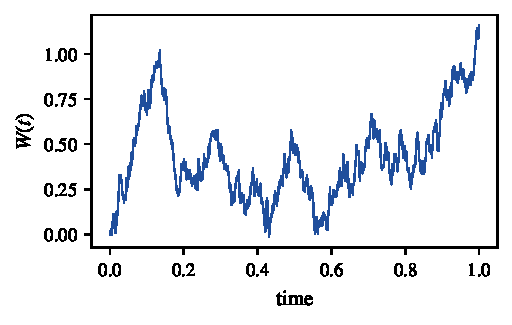
\includegraphics[width=\linewidth]{images/brownian_motion_1d.pdf}
    \caption{One-dimensional Brownian motion (sample path)}
    \label{fig:brownian}
\end{subfigure}\hfill
% Cambia [b] in [t] anche qui
\begin{subfigure}[t]{0.48\textwidth}
    \centering
    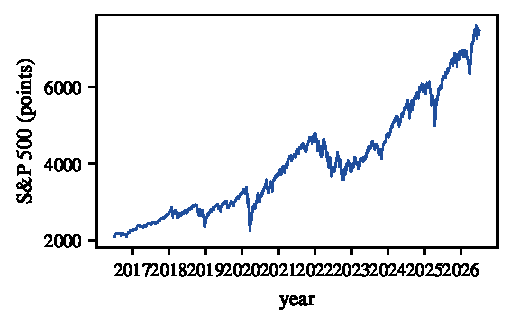
\includegraphics[width=\linewidth]{images/spot_price_sp500.pdf}
    \caption{S\&P\,500 daily closes, 5 July 2016--2 July 2026. Source: cached FRED series SP500.}
    \label{fig:spot}
\end{subfigure}
\end{figure}

This visual similarity is striking given that the two processes originate from very different mechanisms: one is a physical diffusion, the other results from the collective behaviour of many traders responding to supply and demand.



\chapter{Brownian Motion}


\section{Historical observations}
The history of Brownian motion dates back to the early observations of the botanist Robert Brown. While observing pollen grains suspended in a liquid, he noted their highly erratic and jagged trajectory. These particles were subsequently named \textit{Brownian} particles.


\begin{figure}[h!]
    \centering
    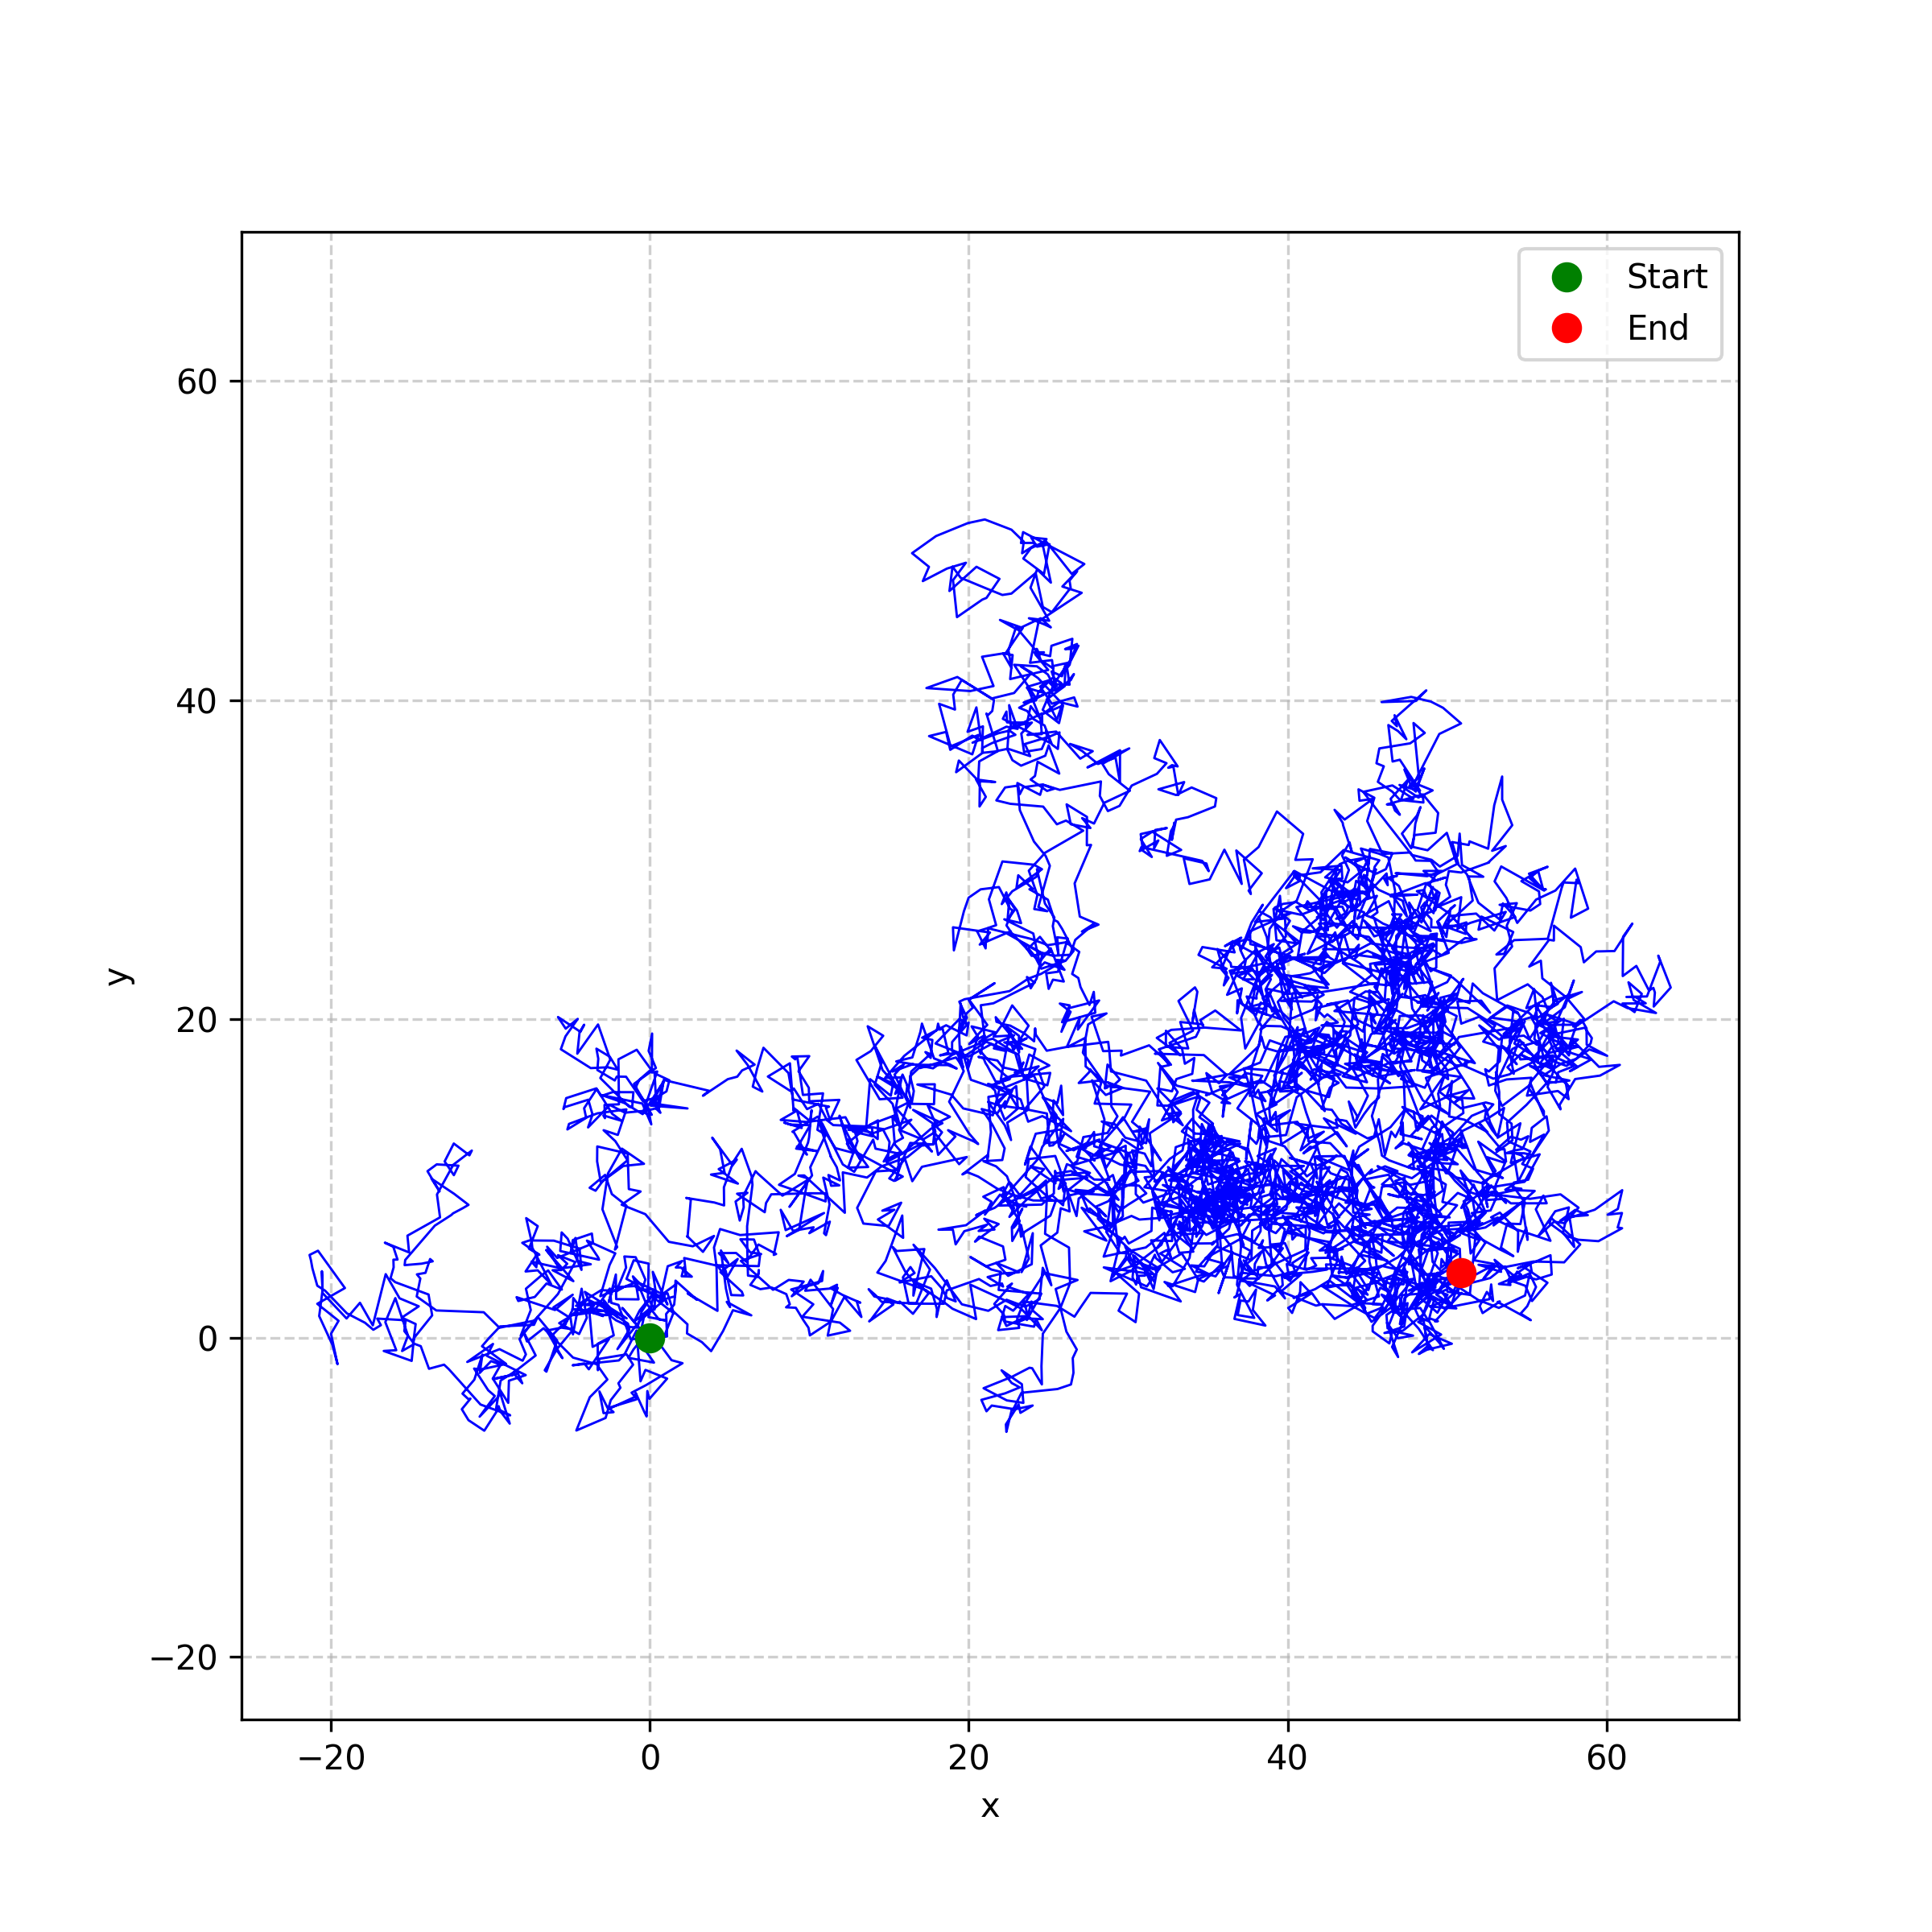
\includegraphics[width=0.6\textwidth]{images/brownian_motion_2d.png}
    \caption{Simulation of a Brownian trajectory in two dimensions.}
\end{figure}

Specifically, Brown made the following qualitative observations:
\begin{enumerate}[label=\roman*)]
    \item The motion never seems to cease.
    \item Different particles always move independently of one another.
    \item The particle's material composition (organic or inorganic) or its mass density do not seem to matter.
    \item The motion becomes faster and more agitated as the fluid's temperature increases or as its viscosity decreases.
    \item The motion exhibits scale invariance (it looks similarly jagged at different magnifications).
    \item The trajectory appears to have no tangent at any point.
\end{enumerate}

The first theoretical characterization of this phenomenon was provided by Albert Einstein in two revolutionary papers published in 1905 \cite{Einstein1905, Einstein1906}. We will now illustrate the key steps of his reasoning.
\section{Einstein's papers}
\subsection{From random walk to the diffusion equation}
He considered a one-dimensional, infinitely extended fluid composed of an ensemble of particles. The Brownian particle undergoes a series of discrete displacements, or "jumps", over very small, successive time intervals, denoted by $\tau$, much smaller than the observation time $T$.


\begin{center}
\begin{tikzpicture}

  \draw[thick] (-3,0) -- (3,0);

  \filldraw[black] (-1,0) circle (2pt);
  \filldraw[black] (1,0) circle (2pt);

  \draw[dashed] (-1,0) arc (180:0:1cm and 0.5cm);

  \node[above] at (0,0.5) {$\Delta$};
\end{tikzpicture}
\end{center}

To describe the statistics of these jumps, Einstein introduced an auxiliary function, $\phi(\Delta)$, which is the probability density function (PDF) for a jump of magnitude $\Delta$. The term $\phi(\Delta)d\Delta$ represents the probability that a single jump has a magnitude between $\Delta$ and $\Delta+d\Delta$. This function is defined by two fundamental properties based on physical reasoning:
\begin{itemize}
    \item \textbf{Normalization}: The particle must perform a jump of some magnitude, so the total probability over all possible jumps must be equal to 1. This is expressed by the normalization condition:
    \begin{equation}
    \int_{-\infty}^{\infty} \phi(\Delta) \,d\Delta = 1.
    \end{equation}
    \item \textbf{Symmetry}: In the absence of any external force or drift, the fluid is isotropic. Therefore, a jump to the right ($+\Delta$) is as probable as a jump of the same magnitude to the left ($-\Delta$). This implies that the function $\phi$ must be an even function:
    \begin{equation}
    \phi(\Delta) = \phi(-\Delta).
    \end{equation}
\end{itemize}

The main goal, however, is to find $p(x,t)$, which represents the number of particles per unit length at position $x$ and time $t$. If we consider $p(x,t)$ as the probability density for a single particle, it must be normalized such that its integral over all space is 1:
\begin{equation}
\int_{-\infty}^{\infty} p(x,t) \,dx = 1.
\end{equation}
The probability of finding the particle in the infinitesimal interval $[x, x+dx]$ is therefore $p(x,t)dx$.

The core idea is to relate the particle density at time $t_f = t+\tau$ to the density at time $t_i = t$. The density of particles at position $x$ at the future time $t+\tau$, denoted $p(x, t+\tau)$, is the sum of probabilities of particles arriving at $x$ from all possible previous positions. A particle that ends up at $x$ must have been at a position $x+\Delta$ at time $t$ and then performed a jump of size $\Delta$. Summing over all possible jumps $\Delta$:
\begin{equation}\label{eq:einstein-master}
p(x, t+\tau) = \int_{-\infty}^{\infty} P(x+\Delta, t) \phi(\Delta) \,d\Delta.
\end{equation}

Now, we perform a Taylor expansion for small $\tau$ and small $\Delta$. The left side is expanded in time:
\begin{equation}
p(x, t+\tau) \approx p(x,t) + \tau \frac{\partial p(x,t)}{\partial t} + \dots;
\end{equation}
the term $p(x+\Delta, t)$ inside the integral is expanded in space around the position $x$:
\begin{equation}
p(x+\Delta, t) \approx p(x,t) + \Delta \frac{\partial p(x,t)}{\partial x} + \frac{\Delta^2}{2} \frac{\partial^2 p(x,t)}{\partial x^2} + \dots;
\end{equation}
substituting these expansions back into Equation~\eqref{eq:einstein-master}:
\begin{equation}
p(x,t) + \tau \frac{\partial P}{\partial t} \approx \int_{-\infty}^{\infty} \left[ p(x,t) + \Delta \frac{\partial p}{\partial x} + \frac{\Delta^2}{2} \frac{\partial^2 p}{\partial x^2} \right] \phi(\Delta) \,d\Delta.
\end{equation}
We can split the integral by linearity:
\begin{equation}
p(x,t) + \tau \frac{\partial p}{\partial t} \approx p(x,t) \underbrace{\int \phi(\Delta)d\Delta}_{=1} + \frac{\partial p}{\partial x} \underbrace{\int \Delta \phi(\Delta)d\Delta}_{=0} + \frac{1}{2}\frac{\partial^2 p}{\partial x^2} \int \Delta^2 \phi(\Delta)d\Delta.
\end{equation}
The terms simplify based on the properties of $\phi$.

So we are left with:
\begin{equation}
\tau \frac{\partial p(x,t)}{\partial t} \approx \frac{1}{2}\frac{\partial^2 p(x,t)}{\partial x^2} \int_{-\infty}^{\infty} \Delta^2 \phi(\Delta) \,d\Delta.
\end{equation}
Dividing by $\tau$, we get:
\begin{equation}
\frac{\partial p(x,t)}{\partial t} = D \frac{\partial^2 p(x,t)}{\partial x^2}.
\end{equation}
This is the \emph{diffusion equation} (with $D=1$ it becomes the well known heat equation), where $D$ is the \emph{diffusion coefficient}, defined as:
\begin{equation}
D := \frac{1}{2\tau} \int_{-\infty}^{\infty} \Delta^2 \phi(\Delta) \,d\Delta.
\end{equation}
Since $\Delta^2 \ge 0$ and $\phi(\Delta) \ge 0$, the integral is positive, thus $D>0$. The dimensions of $D$ are length squared per unit time, $[D] = L^2 T^{-1}$.


\subsection{Solution of the diffusion equation}
We now solve the diffusion equation with a specific initial condition. Physically, it is natural to assume that the process starts with the particle (or all particles) located exactly at the origin at time $t=0$. This condition is represented mathematically by the Dirac delta function, $\delta(x)$. It represents an instantaneous, infinitely concentrated point source. The solution $p(x,t)$ will then describe how this initial certainty "diffuses" into a probability distribution over time.

The problem is thus defined by the partial differential equation and its initial condition:
\begin{equation}\begin{split}
    \frac{\partial p(x,t)}{\partial t} &= D \frac{\partial^2 p(x,t)}{\partial x^2}; \\
    p(x,0) &= \delta(x).
\end{split}\end{equation}
We solve this using the Fourier transform. Let $p(k,t)$ be the Fourier transform of $p(x,t)$ with respect to the spatial variable $x$. The transform pair is defined as:
\begin{equation}\begin{split}
    \text{Inverse Transform:} \quad p(x,t) &= \int_{-\infty}^{\infty} e^{ikx} p(k,t) \,dk; \\
    \text{Transform:} \quad p(k,t) &= \frac{1}{2\pi} \int_{-\infty}^{\infty} e^{-ikx} p(x,t) \,dx.
\end{split}\end{equation}
First, we transform the initial condition. Using the integral representation of the Dirac delta, $\delta(x) = \frac{1}{2\pi} \int e^{ikx} dk$,
\begin{equation}
p(k,0) = \frac{1}{2\pi}.
\end{equation}
Next, we transform the diffusion equation itself. The time derivative remains, while the spatial derivative becomes a multiplication by $(ik)^2 = -k^2$:
\begin{equation}
\mathcal{F}\left[\frac{\partial p}{\partial t}\right] = D \cdot \mathcal{F}\left[\frac{\partial^2 p}{\partial x^2}\right] \implies \frac{\partial p(k,t)}{\partial t} = D(-k^2)p(k,t).
\end{equation}
This transforms the partial differential equation in $(x,t)$ into a simpler ordinary differential equation in the variable $t$ for each value of $k$:
\begin{equation}\begin{split}
    \frac{\partial p(k,t)}{\partial t} &= -Dk^2 p(k,t); \\
    p(k,0) &= \frac{1}{2\pi}.
\end{split}\end{equation}
This is a first-order linear ODE with constant coefficients, which can be solved by separation of variables.

Let's treat $k$ as a constant parameter and solve the ODE for the function $f(t) = p(k,t)$:
\begin{equation}
\frac{df(t)}{dt} = (-Dk^2) f(t).
\end{equation}
Separating the variables $f$ and $t$:
\begin{equation}
\frac{df}{f} = -Dk^2 \,dt.
\end{equation}
Integrating both sides:
\begin{equation}
\int \frac{1}{f} \,df = \int -Dk^2 \,dt \implies \ln|f| = -Dk^2 t + C_0.
\end{equation}
where $C_0$ is the constant of integration. Exponentiating both sides gives:
\begin{equation}
f(t) = e^{-Dk^2 t + C_0} = e^{C_0} e^{-Dk^2 t} = C e^{-Dk^2 t}.
\end{equation}
We find the constant $C$ using the initial condition $p(k,0) = 1/(2\pi)$:
\begin{equation}
p(k,0) = C e^{0} = C \implies C = \frac{1}{2\pi}.
\end{equation}
Thus, the solution in the Fourier space is:
\begin{equation}
p(k,t) = \frac{1}{2\pi} e^{-Dk^2 t}.
\end{equation}

To find the solution in the original space, we apply the inverse Fourier transform to $p(k,t)$:
\begin{equation}
p(x,t) = \int_{-\infty}^{\infty} e^{ikx} p(k,t) \,dk = \frac{1}{2\pi} \int_{-\infty}^{\infty} e^{ikx} e^{-Dk^2 t} \,dk = \frac{1}{2\pi} \int_{-\infty}^{\infty} e^{-Dk^2 t + ikx} \,dk.
\end{equation}
To solve this Gaussian integral, we complete the square in the exponent:
\begin{equation}\begin{split}
-Dtk^2 + ikx &= -Dt \left( k^2 - \frac{ix}{Dt}k \right) \\
             &= -Dt \left[ \left( k - \frac{ix}{2Dt} \right)^2 - \left( \frac{ix}{2Dt} \right)^2 \right] \\
             &= -Dt \left( k - \frac{ix}{2Dt} \right)^2 - Dt \left( \frac{x^2}{4D^2t^2} \right) \\
             &= -Dt \left( k - \frac{ix}{2Dt} \right)^2 - \frac{x^2}{4Dt}.
\end{split}\end{equation}
Substituting this back into the integral:
\begin{equation}
p(x,t) = \frac{1}{2\pi} \int_{-\infty}^{\infty} \exp\left[-Dt\left(k - \frac{ix}{2Dt}\right)^2 - \frac{x^2}{4Dt}\right] \,dk = \frac{1}{2\pi} e^{-\frac{x^2}{4Dt}} \int_{-\infty}^{\infty} e^{-Dt\left(k - \frac{ix}{2Dt}\right)^2} \,dk.
\end{equation}
The remaining integral is a standard Gaussian integral of the form $\int e^{-a(u-b)^2}du = \sqrt{\pi/a}$. Here, $a=Dt$. The complex shift $b=ix/(2Dt)$ does not change the result of the integral over the real line.
\begin{equation}
\int_{-\infty}^{\infty} e^{-Dt\left(k - \frac{ix}{2Dt}\right)^2} \,dk = \sqrt{\frac{\pi}{Dt}}.
\end{equation}
Therefore, the solution is:
\begin{equation}
p(x,t) = \frac{1}{2\pi} e^{-\frac{x^2}{4Dt}} \sqrt{\frac{\pi}{Dt}} = \frac{1}{\sqrt{4\pi Dt}} e^{-\frac{x^2}{4Dt}}.
\end{equation}
This is a Gaussian distribution with mean $\mu=0$ and variance $\sigma^2_t = 2Dt$.

A minimal and standard choice for the diffusion coefficient is $D=1/2$. This specific case defines the standard Brownian motion, also known as the \emph{Wiener process}. The probability density function becomes:
\begin{equation}
p(x,t) = \frac{1}{\sqrt{2\pi t}} e^{-\frac{x^2}{2t}}.
\end{equation}
This process is a cornerstone of stochastic calculus. It exhibits scale invariance and is considered the first and most fundamental example of a 1D fractal process.


\subsection{Physical interpretation and statistical consequences}
The solution we found is a  normal distribution:
\begin{equation}
p(x,t) = \frac{1}{\sqrt{2\pi\sigma_t^2}} e^{-\frac{x^2}{2\sigma_t^2}}.
\end{equation}
where the variance $\sigma_t^2$ is time-dependent:
\begin{equation}
\sigma_t^2 = 2Dt.
\end{equation}


We can calculate the key moments of this distribution.
\begin{itemize}
    \item \textbf{Mean Position}: The average position of the particle is given by the expectation value $\langle x \rangle$. Since the Gaussian is centered at zero (it is an even function) and we are integrating over a symmetric domain, the mean is zero.
    \begin{equation}
    \langle x \rangle = \int_{-\infty}^{\infty} x \, p(x,t) \,dx = 0.
    \end{equation}
    This confirms that the diffusion process has no drift; the particle is equally likely to be found on either side of the origin.

    \item \textbf{Variance}: The variance measures the spread of the distribution.
    \begin{equation}\begin{split}
        \text{Var}[x] &= \langle (x - \langle x \rangle)^2 \rangle = \langle x^2 \rangle - \langle x \rangle^2 = \langle x^2 \rangle \\
        &= \int_{-\infty}^{\infty} x^2 \, p(x,t) \,dx = \sigma_t^2 = 2Dt.
    \end{split}\end{equation}
    This is a very important result of diffusion theory: the variance of the particle's position grows linearly with time. This means the particle spreads out, and our uncertainty about its location increases as time passes. Standard diffusive processes are thus Gaussian.
\end{itemize}

The evolution of the probability density is a macroscopic description of the ensemble of particles, not the path of a single particle. It starts as an infinitely sharp Dirac delta at $t=0$ and then "spreads out" as a Gaussian with increasing width, as illustrated below.

\begin{figure}[h!]
    \centering
    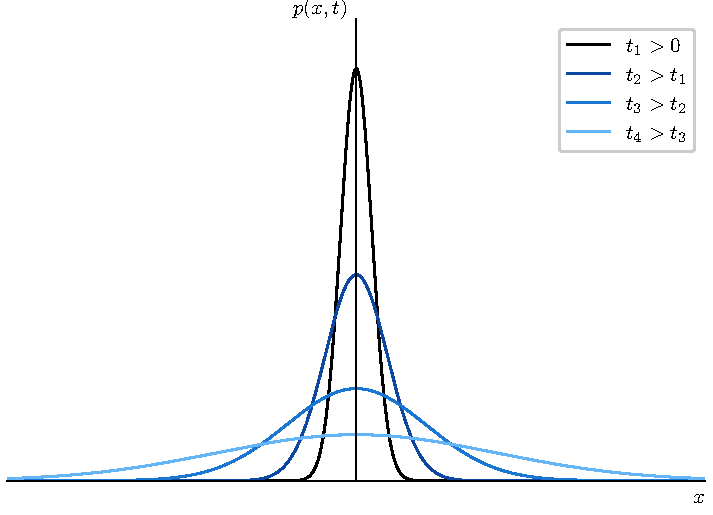
\includegraphics[width=0.8\textwidth]{images/gaussian_evolution.pdf}
    \caption{Evolution of the probability density $p(x,t)$ over time. Starting from a Dirac delta at $t=0$, the distribution spreads out as a Gaussian with variance $\sigma_t^2=2Dt$ increasing linearly in time.}
    \label{fig:gaussian_evolution}
\end{figure}


Another relevant quantity to characterize the displacement of the particle is the Mean Squared Displacement (MSD). It is defined as the average squared distance the particle has traveled from its starting point.
\begin{equation}
\text{MSD}(t) = \langle [x(t) - x(0)]^2 \rangle.
\end{equation}
Let's consider two cases:
\begin{itemize}
    \item If the particle starts at the origin, $x(0)=0$:
    \begin{equation}
    \text{MSD} = \langle [x(t)]^2 \rangle = \langle x^2(t) \rangle = 2Dt.
    \end{equation}
    The MSD is simply the variance.

    \item If the particle starts at a generic position $x(0)=x_0$:
    \begin{equation}\begin{split}
        \text{MSD} &= \langle [x(t) - x_0]^2 \rangle \\
        &= \langle x^2(t)\rangle + x_0^2 - 2x_0  \langle x(t)\rangle\\
        &= \langle x^2(t)\rangle + x_0^2 - 2x_0^2  \\
        & = x_0^2  + 2Dt - x_0^2 \\
        & = 2Dt.
    \end{split}\end{equation}
\end{itemize}
In both cases, the MSD grows linearly with time.

The typical distance traveled by the particle, the mean free path  $\lambda_x$, can be estimated as the root of the MSD.
\begin{equation}
\lambda_x = \sqrt{\text{MSD}} = \sqrt{2Dt}.
\end{equation}
This shows that the characteristic displacement of a diffusing particle grows not with time $t$, but with its square root. This sub-linear growth is a direct consequence of the random, back-and-forth nature of the motion.

\subsection{Einstein's second paper}

Let us now investigate the physical significance of the diffusion coefficient $D$.
We recall from the studies of R. Brown, that the motion of suspended (Brownian) particles becomes more intense as the temperature $T$ rises and as the viscosity $\eta$ of the liquid or the radius $R$ of the particles decrease.
Thus, we need to link these macroscopic parameters (the radius of the particle -- $\sim10^{-6}m$ -- is sufficiently large to neglect quantum effects and consider it a macroscopic object) to the diffusion coefficient.

Let us consider a statistical ensemble of $N$ identical Brownian particles of radius $R$, suspended in a three-dimensional tank liquid of temperature $T$ and viscosity $\eta$ in statistical equilibrium.
We consider three main forces acting on each particle in the vertical direction ($x$):
\begin{itemize}
	\item Gravitational pull:
	\begin{equation}
	F_G=-mg=-\frac{d}{dx}\bigl(V_G(x)\bigr), \qquad V_G(x)=mgx.
	\end{equation}
	\item Archimede's buoyancy:
	\begin{equation}
	F_A(x)=\rho(x)\, g\, Vol \ll F_G \qquad \text{(negligible)}.
	\end{equation}
	\item Stokes drag:
	\begin{equation}
	F_S=-6\pi\eta R v \qquad \text{(valid for low Reynolds' number)},
	\end{equation}
	where the factor $6\pi\eta R$ is also known as the \emph{mobility coefficient}.
	% CLAUDE NOTE: the annotation "coeff. di mobilità" appears in the handwritten notes
	% (PDF 1, page 7) and was previously missing from this section.
\end{itemize}
Restricting our attention to the stationary regime we can define a drift velocity of
\begin{equation}
v_d=\frac{F_G}{6\pi \eta R},
\end{equation}
and a superficial current of matter (number of particles that cross the unit of surface in the unit of time)
\begin{equation}
J_{drift}(x)=v_d\,\rho(x).
\end{equation}
Under the hypothesis of statistical equilibrium and classical physics, Boltzmann formula (see Appendix~\ref{app:ensembles}) entails that
\begin{equation}
\rho(E)=N\frac{e^{-\beta E}}{\mathcal{Z}}, \qquad \beta=(k_BT)^{-1}, \quad E=V(x)+\frac{mv^2}{2}.
\end{equation}
Hence, if we have that $\rho(0)=Ne^{-\beta m v^2/2}$ ($\iff V(0)=0$)
\begin{equation}
	\frac{\rho(x)}{\rho(0)}=e^{-\beta V(x)}.
\end{equation}
This is the case of the gravitational potential $V(x)=V_G(x)=mgx$, which recovers the so-called \textit{barometric distribution}
\begin{equation}
\rho(x)=\rho(0)e^{-\beta m g x}.
\end{equation}
% CLAUDE NOTE: written as in the handwritten notes (PDF 1, page 8), ρ(x) = e^{-βmgx};
% the earlier |F_G| intermediate step was removed at the author's request (2026-07-06).

Since the concentration of the Brownian particles increases with the depth of the liquid, each particle, while falling, experiences an increasing upward "force" generated by the consecutive scattering with other Brownian particles.
The analytic form of the current generated by this effect is nothing more than Fick's diffusion current
\begin{equation}
J_{diff}(x)=-D_{E.S.}\frac{d}{dx}\rho(x),
\end{equation}
for some $D_{E.S.}\in \mathbb{R}^+$ (this is Fick's first law; the second is the diffusion equation itself).
% CLAUDE NOTE: the parenthesis "(la II è quella eq. di diff.)" is in the notes (PDF 1,
% page 7) and was previously missing.
Considering the stationary regime, we demand $\rho(x)$ to be constant over time, \textit{i.e.}, with zero net flow $J_{diff}-J_{drift}=0$.
Identifying $V(x)=Fx$ for some constant force $F=F_G+F_S$,
\begin{equation}
-D\frac{d\rho(x)}{dx}-v_d\rho(x)=0,
\end{equation}
that is,
\begin{equation}
e^{-\beta Fx}\frac{F}{6\pi \eta R}=\rho(x)v_d=-D_{E.S.}\frac{d\rho(x)}{dx}=D_{E.S.}\beta F e^{-\beta F x},
\end{equation}
and simplifying the common exponential factor,
\begin{equation}
D_{E.S.} =\frac{k_BT}{6\pi\eta R},
\end{equation}
where "E.S." stands for Einstein-Smoluchowski.
As a consequence, the variance $\sigma_t^2=2D_{E.S.}t$ varies with the temperature $T$ and the viscosity $\eta$, exactly as in Brown's qualitative observations.
% CLAUDE NOTE: the sentence "dunque la varianza σ_t² varia con T,η" is in the notes
% (PDF 1, page 8) and was previously missing.
With this characterisation, we find all the properties of the chaotic motion described by R. Brown with the exception of self-similarity\footnote{See J. B. Perrin's work for an experimental verification of the Einstein-Smoluchowski formula\cite{Perrin1909}.
Measuring $D$ gives access to $k_B=R/N_A$, hence to an experimental measurement of Avogadro's number $N_A$, in great agreement with the chemical estimate; this earned Perrin the Nobel Prize in 1926.
% CLAUDE NOTE: the k_B = R/N_A remark is in the notes (PDF 1, page 8) and was
% previously missing from this footnote.
}.

Considering a statistical ensemble, we can identify $p(x,t)\leftrightarrow \rho(x,t)$.
% CLAUDE NOTE: the previous version wrote p(x,y), a typo for p(x,t).
Recalling the following formula for Einstein's first work
\begin{equation}\begin{split}
	& \partial_t\rho(x,t)=D\partial_x^2\rho(x,t)\implies\\
	& 0=\partial_t\rho(x,t)-\partial_x\{D\partial_x\rho(x,t)\}=\partial_t\rho(x,t)+\partial_x J(x,t),
\end{split}\end{equation}
recovering a continuity equation for $J(x,t)=-D\partial_x\rho(x,t)$.
In the stationary regime we set $\rho(x,t)\to \rho_S(x)$, entailing that $\partial_t\rho_S=0$ and consequently $\partial_xJ_S=0$.
In this setting, we find $J(x)=-D\partial_x\rho_S(x)$.
This observation fixes $D=D_{E.S.}$.


\section{The Langevin equation}

We now would like to extend Einstein's characterisation of the Brownian motion by describing the trajectory of the Brownian particles.
This, for obvious reasons, cannot be done in a deterministic way, but an attempt to delineate an average trajectory was made by Langevin: his reasoning goes as follows.
Langevin's equation (1908)\cite{Langevin1908} provides a \emph{microscopic} description of the motion, and it is historically the first \emph{stochastic differential equation} --- an object which, at the beginning, had no precise mathematical meaning, and was formalized only later.
% CLAUDE NOTE: the sentence above transcribes the notes' "eq. di Langevin (1908),
% descrizione microscopica → stoch. diff. eq., all'inizio non ha senso matematico,
% viene poi formalizzato" (PDF 1, page 9), previously missing. The formalization is
% the stochastic calculus of Chapter 4.

He considered a statistical ensemble of Brownian particles of mass $m$ and radius $R$ suspended in a 1-dimensional fluid of temperature $T$ and viscosity $\eta$ in statistical equilibrium.
Langevin admits a non-symmetric "jump" distribution, whose unbalance between the probability of a right and a left jump generates an overall drift velocity $v_d$.
The second principle of dynamics can be written as $ma=F=F^{(1)}+F^{(2)}$, with $F^{(1)}=F_S=-6\pi\eta Rv$ the deterministic Stokes force while $F^{(2)}=\xi(t)$ which models the stochastic particles scatterings as \textit{White Noise}.
We choose $\xi(t)$ such that for any time $t$ the ensemble average reads
\begin{equation}
	\langle \xi(t)\rangle_{Ensemble}=0, \;\mathrm{for}\,\,\mathrm{any}\; t\in \mathbb{R}.
\end{equation}
If we consider $\xi(t)\equiv 0$, we find a deterministic differential equation $m\frac{dv(t)}{dt}=-6\pi\eta R v(t)$, which has for a solution $v(t)=v(0)e^{-t/\tau}$, with $\tau=m/6\pi\eta R$.
Considering the full equation instead, it is problematic, because the trajectory it describes turns out not to be differentiable --- a difficulty ignored for the moment (we shall return to it in Chapter~3).
% CLAUDE NOTE: the remark "ma è problematico perché non è derivabile (ignorato per il
% momento)" is in the notes (PDF 1, page 10) and was previously missing.
We have
\begin{equation}\begin{split}
	&m\frac{d^2x}{dt^2}=-6\pi\eta R\frac{dx}{dt}+\xi(t)\\
	& mx\frac{d^2x}{dt^2}=-6\pi\eta Rx\frac{dx}{dt}+x\xi(t)
\end{split}\end{equation}
using the fact that $\frac{d(x^2)}{dt}=2x\frac{dx}{dt}$ and consequently $\frac{d(x^2)}{dt^2}=2(\frac{dx}{dt})^2+2x\frac{d^2x}{dt}$, we have
\begin{equation}\begin{split}
	&\bigg(\frac{m}{2}\bigg)\bigg(2x\frac{d^2x}{dt^2}\bigg)=\bigg(\frac{m}{2}\bigg)\bigg(\frac{d^2(x^2)}{dt^2}-2v^2\bigg),
\end{split}\end{equation}
then, substituting in the previous equation to express everything in function of $x^2$
\begin{equation}\begin{split}
	&\bigg(\frac{m}{2}\bigg)\frac{d^2(x^2)}{dt^2}-mv^2=-3\pi\eta R\frac{d(x^2)}{dt}+x\xi(t).
\end{split}\end{equation}
We observe that $x$ is a stochastic variable since it depends on $\xi(t)$.
In this spirit we evaluate the ensemble average of the differential equation, \textit{i.e.}
\begin{equation}\begin{split}
	&\bigg(\frac{m}{2}\bigg)\frac{d^2}{dt^2}\langle x^2 \rangle-\langle mv^2\rangle =-3\pi\eta R\frac{d}{dt}\langle x^2\rangle +\langle x\xi(t)\rangle.
\end{split}\end{equation}
We recall that under the hypothesis statistical equilibrium, it holds the Equipartition Theorem (Appendix~\ref{app:equipartition}), which entails that $\langle \frac{mv^2}{2}\rangle=\frac{k_BT}{2}$.
In addition, since $\xi(t)$ is independent from the particle's position (\textit{Markov process}), then we can factorise $\langle x\xi(t)\rangle =\langle x\rangle \langle \xi(t)\rangle=0$.
Collecting all of the above observations in one formula, gives
\begin{equation}\begin{split}
	\frac{m}{2}\frac{d^2}{dt^2}\langle x^2 \rangle +3\pi\eta R\frac{d}{dt}\langle x^2\rangle =k_BT.
\end{split}\end{equation}
We observe that, despite in the initial differential equation a stochastic term was added, in the final equation it does not appear: this is because we supposed $\langle \xi(t)\rangle =0$.
However, the trace of its existence lies in the fact that to erase the stochastic term, we had to consider an ensemble-average equation, giving up the "determinability" of our result.

If we set $f(t)=\frac{d}{dt}\langle x^2\rangle$, we have that
\begin{equation}\begin{split}
	&f'(t)+af(t)=b, \;a=6\pi\eta R/m, \;b=2k_BT/m\implies\\
	&f(t)=f_0(t)+f_p(t)=Ce^{-at}+b/a\implies\\
	&\frac{d}{dt}\langle x^2\rangle =Ce^{-\frac{6\pi\eta R t}{m}}+\frac{k_BT}{3\pi\eta R}=Ce^{-t/\tau}+\frac{k_BT}{3\pi\eta R},
\end{split}\end{equation}
with $\tau=m/6\pi\eta R\sim 10^{-8}s$.
After the transient state (\textit{i.e.} for $t>>\tau$) $e^{-t/\tau}\approx 0$, as a consequence, if we integrate the above equation on $[0,t]$ we have that
\begin{equation}\begin{split}
	\langle x^2(t)\rangle =\langle x^2(0)\rangle +\frac{k_BT}{3\pi\eta R}t=\langle x^2(0)\rangle +2t D_{E.S.}.
\end{split}\end{equation}
This result should make the reader "jump on their chair" since it explicitly confirms the equivalence of the macroscopic (statistical -- $p(x,t)$) derivation by Einstein-Smoluchowski with the microscopic (pseudo-deterministic -- $\langle x(t)\rangle$) derivation by Langevin.

The solutions of the Langevin equation constitute a \emph{family of time-dependent trajectories}.
Figure~\ref{fig:brownian-family} shows an ensemble of such trajectories: cutting the family at two successive times, the cross-sections of the cloud are Gaussians with larger and larger variance, exactly the $p(x,t)=\mathcal{N}(0,\,2Dt)$ of the macroscopic description.
% CLAUDE NOTE: "famiglia di traiettorie dipendenti dal tempo" + the pasted plot annotated
% "gaussiane con maggiore varianza" close the Langevin part of the notes (PDF 1, page 10);
% the figure below replaces the pasted plot.

% Figure generated by images/code_for_images/brownian_family.py
\begin{figure}[h!]
\centering
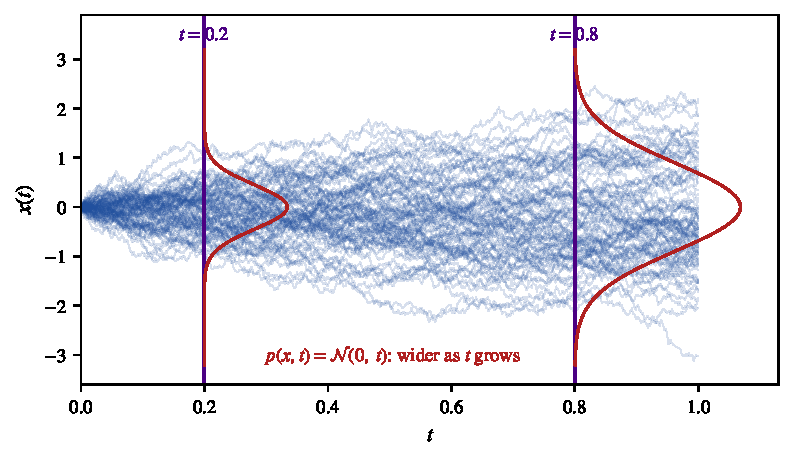
\includegraphics[width=0.85\textwidth]{images/brownian_family.pdf}
\caption{A family of Brownian trajectories, cut at two successive times $t_1=0.2$ and $t_2=0.8$ (vertical lines). The cross-section profiles (red) are Gaussians with variance growing linearly in time --- the microscopic trajectories reconstruct the spreading density of Figure~\ref{fig:gaussian_evolution}. Generated by \texttt{images/code\_for\_images/brownian\_family.py}.}
\label{fig:brownian-family}
\end{figure}


\section{The random walk of Bachelier}

The jump description of Brownian motion admits a discrete formulation of independent interest: the \emph{random walk}.
It was introduced for the first time by Bachelier in his PhD thesis \emph{Th\'eorie de la sp\'eculation} (1900)\cite{Bachelier1900} --- five years \emph{before} Einstein's papers, and with prices, not pollen grains, in mind.

The model rests on four hypotheses.
\begin{enumerate}[label=\roman*)]
    \item The particle can occupy equispaced cells (of width $\Delta x$) on a one-dimensional lattice extending over $(-\infty,+\infty)$.
    \item The initial position is zero at $t=0$.
    \item Calling $P$ the probability of jumping to the right and $q$ the one of jumping to the left, one has $P+q=1$, and the jumps occur regularly, once every interval $\Delta t$.
    (For Einstein, $P=q$.)
    \item The jumps are independent (Markov).
\end{enumerate}
The position is labelled by $m\in\mathbb{Z}$ and $N\in\mathbb{N}$ is the number of jumps performed, so that $N\Delta t$ is the elapsed time.

\begin{center}
\begin{tikzpicture}[scale=1.1]
  \foreach \x in {-2,-1,0,1,2,3}{ \filldraw[black] (\x,0) circle (2pt); }
  \draw[->, thick] (0,0.15) to[bend left=50] node[above]{\small $P$} (0.9,0.15);
  \draw[->, thick] (0,0.15) to[bend right=50] node[above]{\small $q$} (-0.9,0.15);
  \node[below] at (0,-0.12) {\small $m=0$};
  \draw[<->] (2,-0.3) -- (3,-0.3) node[midway, below]{\small $\Delta x$};
\end{tikzpicture}
\end{center}

The question is: what is the probability distribution $P_N(m)$ of being at position $m$ after $N$ jumps?
If $P=\tfrac{1}{2}=q$ the model is the \emph{symmetric} random walk; for $P\ne\tfrac{1}{2}$ and $q=1-P$ the individual jumps are Bernoulli variables, and their sum follows a \emph{binomial distribution}.
The counting is elementary: if the walker performs $m+\ell$ jumps to the right, it must perform $\ell$ jumps to the left, hence $N=m+2\ell$ jumps in total; solving,
\begin{equation}
\ell=\frac{N-m}{2} \ \text{ jumps to the left},
\qquad
m+\frac{N-m}{2}=\frac{N+m}{2} \ \text{ jumps to the right},
\end{equation}
and the binomial distribution is then
\begin{equation}
P_N(m) = \binom{N}{\frac{N+m}{2}}\, P^{\frac{1}{2}(N+m)}\, q^{\frac{1}{2}(N-m)}.
\end{equation}
Normalizing the price to zero at $t=0$, this can be taken as a model for the evolution of prices --- Bachelier's original purpose.

To compute the moments it is convenient to introduce the number of right jumps
\begin{equation}
r:=\frac{N+m}{2},
\qquad
P_N(r)=\binom{N}{r}P^r q^{N-r} = \mathcal{B}(r;P,N),
\end{equation}
for which the standard binomial results follow.
The normalization is immediate from the binomial theorem,
\begin{equation}
\sum_{r=0}^{\infty}\binom{N}{r}P^r q^{N-r} = (P+q)^N = 1,
\end{equation}
the mean is
\begin{equation}
\mathbb{E}[r]=\sum_{r=0}^{\infty} r\,P_N(r) = NP,
\end{equation}
and, from $\mathbb{E}[r^2]=NP+N(N-1)P^2$, the variance is
\begin{equation}
\mathrm{Var}[r]= NP+N(N-1)P^2-N^2P^2 = NP(1-P).
\end{equation}
Translating back to the position through $m=2r-N$,
\begin{equation}
\langle m\rangle = 2\langle r\rangle - N = 2NP-N = 2N\Bigl(P-\frac{1}{2}\Bigr),
\qquad
\mathrm{Var}[m] = 4NP(1-P),
\end{equation}
where we used $\langle m^2\rangle = 4NP(1-P)+4N^2(P-\tfrac{1}{2})^2$.

Both the mean and the variance depend linearly on $N$; but $N=t/\Delta t$, so they are \emph{linear in time} --- recall Einstein's $\sigma_E^2=2Dt$, whose mean vanished because $P=q=\tfrac{1}{2}$.
% CLAUDE NOTE: the notes write "(si ricordi σ_E² = 2Dt, σ_E = 0 perché P=q=½)" (PDF 1,
% page 12); as written, σ_E=0 would contradict σ_E²=2Dt. The intended statement is that
% the MEAN ⟨m⟩ vanishes in the symmetric (Einstein) case, as rendered above.
Note, moreover, that the distribution is a binomial, \emph{not} a Gaussian.

The role of the asymmetry is best seen in three regimes, sketched in Figure~\ref{fig:rw-regimes}.
In the \emph{maximally asymmetric} model ($P=1$, $q=0$, or $P=0$, $q=1$) one has $\mathrm{Var}[m]=0$ and $\mathbb{E}[m]=\pm N$: the walk is purely deterministic.
With $P=\tfrac{3}{4}$, $q=\tfrac{1}{4}$ one finds $\langle m\rangle = N/2$ and $\mathrm{Var}[m]=\tfrac{3}{4}N$: the variable fluctuates around a rising trend.
Finally, with $P=q=\tfrac{1}{2}$, $\langle m\rangle = 0$ and $\mathrm{Var}[m]=N$: pure fluctuation, with the $\sqrt{N}$ fan-out of diffusion.

\begin{figure}[h!]
\centering
\begin{tikzpicture}[scale=0.9]
  % panel 1: deterministic
  \begin{scope}
    \draw[->] (0,0) -- (2.6,0) node[right]{\small $N$};
    \draw[->] (0,-1.3) -- (0,1.5) node[above]{\small $m$};
    \draw[dotted, thick, blue!60!black] (0,0) -- (2.4,1.2) node[right]{\small $\langle m\rangle$};
    \draw[dotted, thick, olive] (0,0) -- (2.4,-1.2) node[right]{\small $\langle m\rangle$};
    \node[below] at (1.3,-1.5) {\small $P=1$ or $q=1$};
  \end{scope}
  % panel 2: asymmetric fluctuating
  \begin{scope}[xshift=5.2cm]
    \draw[->] (0,0) -- (2.6,0) node[right]{\small $N$};
    \draw[->] (0,-1.3) -- (0,1.5) node[above]{\small $m$};
    \draw[dashed] (0,0) -- (2.4,1.0);
    \draw[thick] (0,0) -- (0.3,0.3) -- (0.5,0.1) -- (0.8,0.55) -- (1.0,0.35)
       -- (1.3,0.75) -- (1.5,0.5) -- (1.8,0.95) -- (2.0,0.7) -- (2.3,1.1);
    \node[below] at (1.3,-1.5) {\small $P=\tfrac34,\ q=\tfrac14$};
  \end{scope}
  % panel 3: symmetric
  \begin{scope}[xshift=10.4cm]
    \draw[->] (0,0) -- (2.6,0) node[right]{\small $N$};
    \draw[->] (0,-1.3) -- (0,1.5) node[above]{\small $m$};
    \draw[dotted] (0,0) parabola (2.4,1.1);
    \draw[dotted] (0,0) parabola (2.4,-1.1);
    \draw[thick] (0,0) -- (0.25,0.25) -- (0.45,-0.1) -- (0.7,0.3) -- (0.95,-0.2)
       -- (1.2,-0.55) -- (1.45,-0.25) -- (1.7,-0.7) -- (1.95,-0.35) -- (2.3,0.4);
    \node[below] at (1.3,-1.5) {\small $P=q=\tfrac12$};
  \end{scope}
\end{tikzpicture}
\caption{The three regimes of the random walk: purely deterministic ($P=1$ or $q=1$, zero variance), asymmetric (fluctuations around a linear trend), and symmetric (pure fluctuation inside the $\pm\sqrt{N}$ envelope).}
\label{fig:rw-regimes}
\end{figure}

But this --- Samuelson observed --- cannot be an acceptable model for the fluctuation of prices, because the fluctuations would decrease, which is not what happens.
% CLAUDE NOTE: the notes read "Ma questo (Samuelson) non può essere un modello accettabile
% per la fluttuazione dei prezzi perché le fluttuazioni calerebbero, cosa che non accade"
% (PDF 1, page 12). The explanatory paragraph and the numerical example below were added
% at the author's request (2026-07-06).
The objection deserves to be spelled out, because it is precisely the observation that will lead to the geometric model of Chapter~4.
In an asymmetric random walk the mean position grows linearly, $\langle m\rangle \propto N$, while the spread grows only as a square root, $\mathrm{s.d.}[m] = \sqrt{4NPq} \propto \sqrt{N}$; the fluctuations \emph{relative to the price level} therefore decay,
\begin{equation}
\frac{\mathrm{s.d.}[m]}{\langle m\rangle} \propto \frac{\sqrt{N}}{N} = \frac{1}{\sqrt{N}} \;\xrightarrow{\ N\to\infty\ }\; 0,
\end{equation}
and an asset following this model would become, in proportion to its own value, ever quieter as it grows.
A concrete example makes the failure vivid.
Take a stock worth 100\,\euro{} today, fluctuating by about 1\,\euro{} per day (one percent), and suppose that over the years its price drifts up tenfold, to 1000\,\euro.
The arithmetic model predicts that its daily fluctuations are \emph{still} of the order of 1\,\euro{} --- now a mere $0.1\%$ of the price --- whereas a real thousand-euro stock keeps fluctuating by percentage points, that is, by tens of euros per day.
What is statistically stationary in real markets is the \emph{relative} return, not the absolute increment: the fluctuations must be proportional to the price itself, which is exactly the multiplicative structure of the geometric Brownian motion of Chapter~4.

\subsection{The continuum limit}

The Gaussian is recovered from the binomial in the \emph{continuum limit}.
Define the physical variables
\begin{equation}
x:=m\Delta x, \qquad t:=N\Delta t,
\end{equation}
so that the mean position becomes
\begin{equation}
\langle x\rangle = \langle m\rangle\,\Delta x = (2P-1)N\Delta x = (2P-1)\frac{t}{\Delta t}\Delta x,
\end{equation}
and, introducing the velocity
\begin{equation}
v:=\lim_{\substack{\Delta x\to0\\ \Delta t\to0}} (2P-1)\frac{\Delta x}{\Delta t}
\qquad \text{(the limit does not exist by itself: it is heuristic)},
\end{equation}
one finds $\langle x\rangle = v\,t$: a \emph{drift} term.
For the variance,
\begin{equation}
\mathrm{Var}[x] = \bigl\{\langle m^2\rangle - \langle m\rangle^2\bigr\}(\Delta x)^2 = 4Pq\,(\Delta x)^2\frac{t}{\Delta t},
\end{equation}
and defining the diffusion coefficient
\begin{equation}
D := \lim_{\substack{\Delta x\to0\\ \Delta t\to0}} 2Pq\,\frac{(\Delta x)^2}{\Delta t},
\qquad\text{it follows that}\qquad
\mathrm{Var}[x]=2Dt.
\end{equation}

The Gaussian solution is contained in Bachelier's model.
Indeed, for $P$ fixed and $N\to\infty$,
\begin{equation}
P_N(m)=\mathcal{B}(m;P,N) \;\longrightarrow\; P_G(m),
\qquad
P_G(m) = \frac{1}{\sqrt{2\pi\,4NPq}}\,\exp\Bigl\{-\frac{(m-\langle m\rangle)^2}{2\,(4NPq)}\Bigr\},
\end{equation}
a correctly normalized Gaussian: this is a particular case of the central limit theorem, known as the \emph{De Moivre--Laplace theorem}.
Passing to the physical variables, $m\to x=m\Delta x$ and $N\to t=N\Delta t$, some algebra and the continuum limit give
\begin{equation}
P_N(m,N) \;\longrightarrow\; P_N(m\Delta x, N\Delta t)\,\Delta x
\;\xrightarrow[\Delta t\to0]{\Delta x\to0}\;
\frac{1}{\sqrt{4\pi Dt}}\,\exp\Bigl\{-\frac{(x-vt)^2}{4Dt}\Bigr\}\,dx = P_G(x,t)\,dx,
\end{equation}
a Gaussian with $\langle x\rangle = vt$ and $\mathrm{Var}[x]=2Dt$: Einstein's solution, with a drift.

\subsection{From the master equation to the Fokker--Planck equation}

But where does this Gaussian come from?
In the discrete case, the probability of being at $x$ at time $t+\Delta t$ obeys the \emph{master equation}
\begin{equation}
P(x,t+\Delta t) = P\,P(x-\Delta x,t) + q\,P(x+\Delta x,t),
\end{equation}
since the walker must arrive either from the left (with probability $P$) or from the right (with probability $q$).
Expanding the left side in time,
\begin{equation}
P(x,t+\Delta t) = P(x,t) + \Delta t\,\frac{\partial P}{\partial t},
\end{equation}
and each term on the right in space,
\begin{equation}\begin{split}
P\,P(x-\Delta x,t) + q\,P(x+\Delta x,t)
&= P\Bigl[P(x,t) - \Delta x\frac{\partial P}{\partial x} + \frac{\Delta x^2}{2}\frac{\partial^2 P}{\partial x^2}\Bigr]\\
&\quad + q\Bigl[P(x,t) + \Delta x\frac{\partial P}{\partial x} + \frac{\Delta x^2}{2}\frac{\partial^2 P}{\partial x^2}\Bigr],
\end{split}\end{equation}
which reassembles into
\begin{equation}
\underbrace{(P+q)}_{=1} P(x,t) + \underbrace{(-P+q)}_{1-2P}\,\Delta x\,\frac{\partial P}{\partial x} + \underbrace{(P+q)}_{=1}\,\frac{\Delta x^2}{2}\,\frac{\partial^2 P}{\partial x^2}.
\end{equation}
Therefore, dividing by $\Delta t$ (the terms $P(x,t)/\Delta t$ cancel between the two sides),
\begin{equation}
\frac{\partial P}{\partial t} = (1-2P)\frac{\Delta x}{\Delta t}\frac{\partial P}{\partial x} + \frac{1}{2}\frac{\Delta x^2}{\Delta t}\frac{\partial^2 P}{\partial x^2},
\end{equation}
and with the definitions of $v$ and $D$ given above (with $P=q=\tfrac12$), in the continuum\footnote{A small bookkeeping subtlety: the expansion produces the diffusion coefficient $\tfrac12\Delta x^2/\Delta t$, while the variance-based definition given earlier is $D = 2Pq\,\Delta x^2/\Delta t$; the two coincide exactly at $P=q=\tfrac12$ ($4Pq=1$), which is why the derivation specifies this case.
In the joint limit $\Delta x,\Delta t\to0$ with $v$ and $D$ finite, $P\to\tfrac12$ automatically, so no inconsistency survives in the continuum.}
% CLAUDE NOTE: the bookkeeping remark was promoted from a source comment to the footnote
% above at the author's request (2026-07-06).
\begin{equation}
\frac{\partial}{\partial t}P(x,t) = \underbrace{D\frac{\partial^2}{\partial x^2}P(x,t)}_{\text{pure diffusion}} - \underbrace{v\frac{\partial}{\partial x}P(x,t)}_{\text{drift}},
\end{equation}
without the drift term when $\langle x\rangle=0$.
This is the \emph{Fokker--Planck equation} --- here obtained for the simplest of all processes, and derived in full generality in Chapter~3.


\section{The central limit theorem}

The Gaussian appeared twice in this chapter --- as the solution of the diffusion equation and as the limit of the binomial --- and this is no coincidence: behind both stands the \emph{central limit theorem} (CLT), which we now state, prove, and (importantly for what comes later in this book) criticize.

\medskip
\noindent\textbf{Theorem (CLT).}
\emph{Let $\{X_i\}_i$ be random variables and $S_N:=\sum_{i=1}^{N}X_i$ their sum; then, for $N\to\infty$, $S_N$ tends to a Gaussian, provided that (a) the $X_i$ are i.i.d.\ (independent and identically distributed), and (b) the mean $\langle X_i\rangle$ and the variance $\mathrm{Var}[X_i]$ exist finite for every $i$.}
\medskip

The two hypotheses look innocent; the critique of L\'evy and Mandelbrot, to which we return at the end of the section, is aimed precisely at them.

\subsection{Characteristic functions}

The proof (due to Lindeberg and L\'evy) rests on the \emph{characteristic function}: given a density $P(x)$ on $\mathbb{R}$,
\begin{equation}
\varphi(k) := \int_{\mathbb{R}} dx\, e^{ikx}\,P(x) = \mathcal{F}[P] = \mathbb{E}\bigl[e^{ikx}\bigr],
\qquad
P(x) = \frac{1}{2\pi}\int_{\mathbb{R}} dk\, e^{-ikx}\,\varphi(k),
\end{equation}
i.e.\ the Fourier transform of the density.
Two properties make it the perfect tool.

\paragraph{a) Convolution theorem.}
Since $\mathcal{F}[f*g]=\mathcal{F}[f]\cdot\mathcal{F}[g]$, sums of independent variables become products of characteristic functions.
Explicitly: for $X_1$ and $X_2$ i.i.d., the sum $S_2:=X_1+X_2$ is again random, and its density is obtained by extracting the two variables, $P(x_1,x_2)=P(x_1)P(x_2)=P(S_2-x_1)P(x_1)$, and summing over all the possible ways of realizing $S_2$:
\begin{equation}
P_2(S_2)=\int_{\mathbb{R}} P(S_2-x_1)\,P(x_1)\,dx_1,
\end{equation}
the convolution of two identical densities.
Transforming,
\begin{equation}
\mathcal{F}[P_2]=\mathcal{F}[P*P]=\varphi_2(k)=\mathcal{F}[P]\,\mathcal{F}[P]=\varphi^2(k),
\end{equation}
and iterating,
\begin{equation}
\mathcal{F}[P_N]=\varphi_N(k)=\varphi^N(k).
\end{equation}

\paragraph{b) Moment expansion.}
Expanding $e^{ikx}=\sum_{m=0}^{\infty}\frac{(ik)^m}{m!}x^m$ inside the transform,
\begin{equation}
\varphi(k)=\int_{\mathbb{R}} dx\, e^{ikx}P(x) = \sum_{m=0}^{\infty}\frac{(ik)^m}{m!}\int_{\mathbb{R}} dx\, x^m P(x) = \sum_{m=0}^{\infty}\frac{(ik)^m}{m!}\langle x^m\rangle,
\end{equation}
\emph{only if the moments exist} (i.e.\ the integrals converge) --- but it happens that infinitely many do not~(!), and this is where the critique will strike.
Conversely, the moments are read off the derivatives at the origin:
\begin{equation}
\frac{d^\ell}{dk^\ell}\varphi(k)\Big|_{k=0} = i^\ell\int_{\mathbb{R}} dx\, x^\ell\,P(x) = i^\ell\langle x^\ell\rangle
\quad\Longrightarrow\quad
\langle x^\ell\rangle = (-i)^\ell\,\frac{d^\ell}{dk^\ell}\varphi(k)\Big|_{k=0},
\qquad \forall\,\ell,
\end{equation}
% CLAUDE NOTE: the notes write "⟨x^ℓ⟩ = −i^ℓ d^ℓ/dx^ℓ φ(k)|_{k=0}" (PDF 1, page 16):
% the derivative is with respect to k (not x), and the prefactor is (−i)^ℓ; both slips
% of fast handwriting, rendered correctly above.
so that from $\varphi(k)$ one reconstructs the whole distribution.

\subsection{Proof of the theorem}

We standardize first.
Let $\mu:=\langle X_i\rangle$ and $\sigma^2:=\mathrm{Var}[X_i]$ (equal for all $i$ because the variables are identically distributed, but the argument generalizes), and define
\begin{equation}
X_i \;\longrightarrow\; \xi_i := \frac{X_i-\mu}{\sigma},
\qquad
\langle\xi_i\rangle = 0, \quad \mathrm{Var}[\xi_i]=1,
\end{equation}
rescaling then each variable by $\sqrt{N}$, $\xi_i\mapsto \xi_i/\sqrt{N}$.
The standardized sum
\begin{equation}
S_N := \frac{1}{\sqrt{N}}\sum_{i=1}^{N}\xi_i,
\qquad
\langle S_N\rangle = \frac{1}{\sqrt{N}}\sum_i \langle\xi_i\rangle = 0,
\quad
\mathrm{Var}[S_N] = \langle S_N^2\rangle = \frac{1}{N}\sum_{i=1}^{N}\langle\xi_i^2\rangle = 1,
\end{equation}
remains itself standardized.
We must show that $P(S_N)=P_G(S_N)=\mathcal{N}(0,1)$, and we do so by showing that the two have the same characteristic function.

Each rescaled variable contributes $\mathbb{E}\bigl[e^{ik\xi_i/\sqrt{N}}\bigr]=\varphi\bigl(\tfrac{k}{\sqrt{N}}\bigr)$ for every $\xi_i$, so by the convolution theorem
\begin{equation}
\varphi_N(k) = \Bigl[\varphi\Bigl(\frac{k}{\sqrt{N}}\Bigr)\Bigr]^{N}.
\end{equation}
Expanding in moments,
\begin{equation}
\varphi\Bigl(\frac{k}{\sqrt{N}}\Bigr) \approx 1 + \frac{ik}{\sqrt{N}}\underbrace{\langle\xi_i\rangle}_{=0} - \frac{k^2}{2N}\underbrace{\mathrm{Var}[\xi_i]}_{=1} - \frac{i}{3!}\frac{k^3}{N^{3/2}}\langle\xi_i^3\rangle + \frac{1}{4!}\frac{k^4}{N^2}\langle\xi_i^4\rangle + \dots,
% CLAUDE NOTE: the notes (PDF 1, page 16) write the third and fourth terms with flipped
% signs (+i/3!... and −1/4!...); corrected here at the author's request (2026-07-06),
% since (ik)³ = −ik³ and (ik)⁴ = +k⁴. The slip was inconsequential, as these terms are
% suppressed for N→∞ and dropped in the next step.
\end{equation}
where $\langle\xi_i^3\rangle$ is the \emph{skewness}, the parameter of asymmetry (zero if the distribution is symmetric), and $\langle\xi_i^4\rangle$ is the \emph{kurtosis}, the parameter of the behaviour of the tails (heavy tails).
Almost all the known distributions have their higher moments defined, and for large $N$ these are negligible with respect to the first two; therefore
\begin{equation}
\varphi_N(k) \approx \Bigl(1-\frac{k^2}{2N}\Bigr)^{N},
\qquad
\lim_{N\to\infty}\varphi_N(k) = \lim_{N\to\infty}\Bigl(1-\frac{k^2}{2N}\Bigr)^{N} = e^{-k^2/2},
\end{equation}
using $(1+\tfrac{a}{x})^x\xrightarrow{x\to\infty}e^a$.
Inverting the transform, by completing the square exactly as in the solution of the diffusion equation,
\begin{equation}\begin{split}
P(S_N) &= \frac{1}{2\pi}\int_{\mathbb{R}} dk\, e^{-k^2/2}\,e^{-ikS_N}\\
&= \frac{1}{2\pi}\int_{\mathbb{R}} dk\, e^{-\frac{1}{2}(k+iS_N)^2}\,e^{-S_N^2/2}
= \frac{1}{\sqrt{2\pi}}\,e^{-S_N^2/2}:
\end{split}\end{equation}
a Gaussian with mean $0$ and variance $1$. $\blacksquare$

\subsection{Critical remarks}

The theorem is powerful, but each of its hypotheses deserves interrogation --- and the answers open the door to the econophysics of Chapter~7.
\begin{itemize}
    \item \emph{Does it hold if the variables are not independent?} No.
    \item \emph{If they are not identically distributed?} Yes --- but no single variable must dominate the others.
    \item \emph{Is the asymptotic limit necessary?} No (the Berry--Esseen theorem controls the finite-$N$ error), but the summands must be \emph{stable}: invariant in form under addition and convolution.
    \item \emph{Can it hold if the mean and/or the variance do not exist?} No.
    Do similar PDFs exist? Yes: the \emph{L\'evy-stable distributions} --- which turn out to be better at describing real data.
    And does a form of the theorem exist for variables drawn from L\'evy-stable laws? Yes: the \emph{generalized CLT}, whose limit is not a Gaussian.
    \item \emph{If mean, variance and skewness exist, but the kurtosis does not, does the CLT hold?}
    There exist distributions of this kind: e.g.\ the Student-$t$, $P_S(x,\nu)$, with $\nu$ degrees of freedom, for which $\nu\to\infty$ gives $P_S\to P_G(0,1)$; or the Tsallis distribution, $P_t(x,q)\xrightarrow{q\to1}\mathcal{N}(0,1)$; here $q,\nu$ are shape parameters.
    Such distributions are \emph{leptokurtic}: sharper at the centre and heavier in the tails than the Gaussian (Figure~\ref{fig:leptokurtic}; the case $\nu=3$ will star in Chapter~7).
    The sum of many $P_S$ variables does reproduce a Gaussian \emph{at the centre} --- which makes sense, since mean and variance refer to the central part --- but the convergence is very slow (sums of order $10^2$).
\end{itemize}

\begin{figure}[h!]
\centering
\begin{tikzpicture}[scale=1.1]
    \draw[->] (-3.2,0) -- (3.4,0) node[right]{$x$};
    \draw[->] (0,-0.2) -- (0,2.6) node[above]{$P(x)$};
    \draw[thick, domain=-3:3, samples=80] plot (\x, {2.0*exp(-\x*\x/1.1)});
    \draw[thick, teal, domain=-3:3, samples=80] plot (\x, {2.3/((1+\x*\x/1.5)^2)});
    \node[teal, font=\footnotesize, align=left] at (2.6,1.6) {leptokurtic\\ (heavy tails)};
    \node[font=\footnotesize] at (-2.3,1.0) {Gaussian};
\end{tikzpicture}
\caption{A leptokurtic distribution (teal) against a Gaussian of the same scale: sharper peak at the centre, heavier tails far out. Sums of such variables re-Gaussianize only in the central region, and very slowly.}
\label{fig:leptokurtic}
\end{figure}

The most famous L\'evy-stable law is the \emph{Cauchy} distribution,
\begin{equation}
P_c(x)=\frac{\gamma}{\pi}\,\frac{1}{x^2+\gamma^2},
\qquad \gamma \text{ of scale},
\end{equation}
for which the pathology can be checked by hand: with $\gamma=1$,
\begin{equation}\begin{split}
\langle x^2\rangle &= \frac{1}{\pi}\int_{\mathbb{R}} x^2\,\frac{1}{x^2+1}\,dx\\
&= \frac{2}{\pi}\biggl\{\int_0^{\infty}\!dx\,\frac{x^2+1}{x^2+1} - \int_0^{\infty}\!dx\,\frac{1}{x^2+1}\biggr\}\\
&= \frac{2}{\pi}\Bigl[x-\arctan x\Bigr]_0^{+\infty} = +\infty,
\end{split}\end{equation}
and $\langle x\rangle = \infty$ --- more precisely, the integral defining the mean is not absolutely convergent (its principal value is zero), so the mean is in fact \emph{undefined} rather than infinite.
% CLAUDE NOTE: the notes write "⟨x⟩ = ∞" (PDF 1, page 17); the clarification about
% absolute convergence was promoted from this comment into the text at the author's
% request (2026-07-06). The second moment is genuinely +∞.
More generally, a L\'evy-stable density $P_\alpha(x)$ behaves asymptotically as
\begin{equation}
P_\alpha(x) \;\xrightarrow{|x|\to\infty}\; \frac{1}{|x|^{1+\alpha}},
\qquad 0<\alpha\le2,
\end{equation}
interpolating between the Gaussian ($\alpha=2$) and pure power laws: for $0<\alpha<1$ neither the mean nor the variance exist; for $1<\alpha<2$ the variance does not exist.
And summing Cauchy variables? Still a Cauchy: the L\'evy-stable laws \emph{replicate themselves} under addition --- they are the fixed points that the generalized CLT converges to, as the Gaussian is for the classical one.
All of this is taken up quantitatively in Chapter~7, where these distributions meet financial data.

Mandelbrot's verdict on the classical hypotheses may serve as the epigraph for that chapter: \emph{``physicists think the whole world is Gaussian''}.


\chapter{Stochastic Processes}

In the previous chapter Brownian motion appeared twice, and in two rather different guises: as a macroscopic diffusion process, governed by a partial differential equation for a density, and as the microscopic, erratic trajectory of a suspended particle.
It is natural to ask what these two descriptions have in common, and whether they are instances of something more general.
They are.
In this chapter we step back and develop the general formalism of \emph{stochastic processes}, of which Brownian motion is the most fundamental example.
Our goal is to construct, in full generality, the equation that governs the evolution in time of the probability density of a random variable, and to identify the conditions under which this equation takes the manageable form of a \emph{Fokker--Planck equation}.
Everything we do later in this book --- from option pricing to the distribution of wealth --- rests on the machinery built here.


\section{General formalism}

A \emph{stochastic process} is a system that evolves in time in a probabilistic way.
Physically, it is the probabilistic counterpart of a dynamical system: the time evolution is still governed by a law, but the law prescribes probabilities rather than certainties.
% CLAUDE NOTE: the "physical definition" sentence follows the course slides
% (Processi Stocastici: definizioni & classificazione), added 2026-07-06.
Formally, it is a family of random variables
\begin{equation}
\{X(t),\, t\in T\},
\end{equation}
indexed by a time parameter $t$ that runs over a (non-numerable) set $T$.
Two cases occur in practice.
If time is \emph{discrete}, $T=\mathbb{N}$, the process is a sequence $X(t=t_n)=X_n$; if time is \emph{continuous}, $T=\mathbb{R}^+$, the process is a function $X(t)=x(t)$.
We will mostly work in continuous time, although discretization will reappear whenever we need to actually compute something.

A particular sequence of values produced by the process is a \emph{realization}, or \emph{trajectory}.
When the sequence comes from real observations, one speaks of a \emph{historical time series}.
The set of all possible realizations is called the \emph{ensemble} (or \emph{phase space}), visualized in Figure~\ref{fig:ensemble}: a stochastic process is an infinite family of functions evolving randomly in time, and cutting the family at a fixed time $t_0$ defines the random variable $X(t_0)$.
The distinction matters: an experimentalist --- or a trader --- only ever observes \emph{one} realization, whereas the theory speaks about the whole ensemble.
We will meet the consequences of this tension more than once.

% Figure after the course slides (Processi Stocastici: definizioni & classificazione);
% generated by images/code_for_images/ensemble.py
\begin{figure}[h!]
\centering
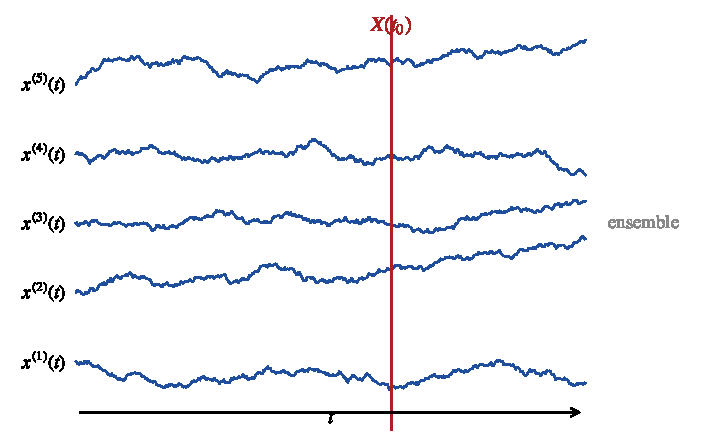
\includegraphics[width=0.7\textwidth]{images/ensemble.pdf}
\caption{Realizations and ensemble. Each curve $x^{(k)}(t)$ is one realization of the same stochastic process; the collection of all of them is the ensemble (phase space). Fixing a time $t_0$ (vertical cut) turns the process into an ordinary random variable $X(t_0)$, whose statistics is taken \emph{across} the realizations. Generated by \texttt{images/code\_for\_images/ensemble.py}.}
\label{fig:ensemble}
\end{figure}

At the statistical level, the process is completely characterized by its \emph{joint probability density}
\begin{equation}
P_n(x_n,t_n;\,x_{n-1},t_{n-1};\dots;x_1,t_1) \equiv P_n,
\end{equation}
which gives the probability density of observing the value $x_1$ at time $t_1$, the value $x_2$ at time $t_2$, and so on.
We adopt throughout the \emph{forward} ordering of the times; the backward ordering gives an equivalent description.
That the whole hierarchy $\{P_n\}$ really is all there is to know is the content of a classical result.

\medskip
\noindent\textbf{Theorem (Kolmogorov).}\cite{Kolmogorov1931}
\emph{A stochastic process is uniquely defined once the finite-dimensional joint probability density is assigned for every finite set of times $\{t_1,t_2,\dots,t_n\}\in T$.}
\medskip

The hierarchy of joint densities cannot be arbitrary, however: it must satisfy four consistency conditions.
\begin{enumerate}
    \item \textbf{Positivity}: each density is non-negative,
    \begin{equation}
    P_n \ge 0.
    \end{equation}
    \item \textbf{Symmetry}: the density is invariant under any permutation of its $(x_i,t_i)$ pairs,
    \begin{equation}
    P_n(\dots;x_i,t_i;\dots;x_j,t_j;\dots) = P_n(\dots;x_j,t_j;\dots;x_i,t_i;\dots).
    \end{equation}
    \item \textbf{Completeness} (marginalization): integrating out the most recent variable lowers the order of the hierarchy,
    \begin{equation}
    \int_{-\infty}^{\infty} P_n(x_n,t_n;\dots;x_1,t_1)\,dx_n = P_{n-1}(x_{n-1},t_{n-1};\dots;x_1,t_1).
    \end{equation}
    \item \textbf{Normalization}: the one-time density integrates to one,
    \begin{equation}
    \int_{-\infty}^{\infty} P_1(x,t)\,dx = 1.
    \end{equation}
\end{enumerate}
These conditions look innocuous, but completeness in particular will do real work for us shortly: it is the seed of the Chapman--Kolmogorov equation.

Two special classes of processes deserve a name.
A process is \emph{stationary} when the joint density is invariant under a global translation of all the times,
\begin{equation}
P_n(x_n,t_n+\Delta t;\dots;x_1,t_1+\Delta t) = P_n(x_n,t_n;\dots;x_1,t_1),
\end{equation}
so that only time \emph{differences} matter; in particular the one-time density becomes time independent, $P(x,t)=P(x)$.
A process is instead \emph{purely random} when there is no correlation at all between different times: for every $m$ and every $t_1\le\dots\le t_m$,
\begin{equation}
P(x_m,t_m\mid x_{m-1},t_{m-1};\dots;x_1,t_1) = P(x_m,t_m),
\end{equation}
so that the joint density factorizes completely,
\begin{equation}
P_m(x_m,t_m;\dots;x_1,t_1) = \prod_{i=1}^{m} P(x_i,t_i).
\end{equation}
A purely random process has no dynamics worth the name: each instant is drawn afresh, oblivious of everything that came before.

In writing the last definitions we have used the \emph{conditional} density, defined as
\begin{equation}
P(x_m,t_m\mid x_{m-1},t_{m-1};\dots;x_1,t_1) := \frac{P_m(x_m,t_m;x_{m-1},t_{m-1};\dots;x_1,t_1)}{P_{m-1}(x_{m-1},t_{m-1};\dots;x_1,t_1)},
\end{equation}
from which the \emph{Bayes theorem} follows immediately,
\begin{equation}
P_2(x_2,t_2;x_1,t_1) = P(x_2,t_2\mid x_1,t_1)\,P_1(x_1,t_1).
\end{equation}
The conditional density answers the question that any observer actually asks: \emph{given} what I have seen so far, what happens next?


\section{Markov processes and the Chapman--Kolmogorov equation}

Between the two extremes of a purely random process (no memory at all) and a general process (arbitrarily long memory) lies the class that dominates applications.
A process is a \emph{Markov process} when the conditional density depends only on the most recent time,
\begin{equation}
P(x_m,t_m\mid x_{m-1},t_{m-1};\dots;x_1,t_1) = P(x_m,t_m\mid x_{m-1},t_{m-1}),
\qquad \forall m,\ \forall t_1\le\dots\le t_m.
\end{equation}
In words: knowledge of the present determines the statistics of the future, with no memory of the past.
A typical example is the tossing of coins in succession in time.
Whether \emph{prices} are Markovian is a far deeper question, and one to which we shall return in Chapter~5.

The Markov property has two consequences that between them carry the entire chapter.

\paragraph{1) Structure of the joint density.}
By definition of the conditional density,
\begin{equation}\begin{split}
P(x_m,t_m\mid x_{m-1},t_{m-1};\dots;x_1,t_1)
&= \frac{P_m(x_m,t_m;x_{m-1},t_{m-1};\dots;x_1,t_1)}{P_{m-1}(x_{m-1},t_{m-1};\dots;x_1,t_1)}\\
&= P(x_m,t_m\mid x_{m-1},t_{m-1}),
\end{split}\end{equation}
from which
\begin{equation}
P_m(x_m,t_m;\dots;x_1,t_1) = P(x_m,t_m\mid x_{m-1},t_{m-1})\,P_{m-1}(x_{m-1},t_{m-1};\dots;x_1,t_1).
\end{equation}
The same identity applied to $P_{m-1}$ gives
\begin{equation}
P_{m-1}(x_{m-1},t_{m-1};x_{m-2},t_{m-2};\dots) = P(x_{m-1},t_{m-1}\mid x_{m-2},t_{m-2})\,P_{m-2}(x_{m-2},t_{m-2};\dots),
\end{equation}
and therefore
\begin{equation}
P_m = P(x_m,t_m\mid x_{m-1},t_{m-1})\,P(x_{m-1},t_{m-1}\mid x_{m-2},t_{m-2})\,P_{m-2}.
\end{equation}
Iterating all the way down to $P_1$, we obtain
\begin{equation}
P_m(x_m,t_m;\dots;x_1,t_1) = \prod_{j=2}^{m} \underbrace{P(x_j,t_j\mid x_{j-1},t_{j-1})}_{\text{transition probability (in } t_j-t_{j-1})}\ \underbrace{P(x_1,t_1)}_{\text{assigned condition}}.
\end{equation}
This is a remarkable simplification.
A Markov process is entirely built out of two ingredients: the \emph{transition probabilities} $P(x_j,t_j\mid x_{j-1},t_{j-1})$, which propagate the process one step at a time, and the initial one-time density.
Instead of an infinite hierarchy of joint densities, we need to understand a single object --- the transition probability --- and everything else follows.

\paragraph{2) Linking points in time: the Chapman--Kolmogorov equation.}
The first non-trivial case of the product formula is $m=3$, and it hides an integral equation.
From the result above,
\begin{equation}
P_3(x_3,t_3;x_2,t_2;x_1,t_1) = P(x_3,t_3\mid x_2,t_2)\,P(x_2,t_2\mid x_1,t_1)\,P_1(x_1,t_1).
\end{equation}
Let us integrate over the intermediate value $x_2$ and use the completeness condition of the previous section,
\begin{equation}\begin{split}
\int_{\mathbb{R}} dx_2\, P_3(x_3,t_3;x_2,t_2;x_1,t_1)
&\overset{\text{compl.}}{=} P_2(x_3,t_3;x_1,t_1)\\
&= P_1(x_1,t_1)\int_{\mathbb{R}} dx_2\, P(x_3,t_3\mid x_2,t_2)\,P(x_2,t_2\mid x_1,t_1).
\end{split}\end{equation}
On the other hand, Bayes gives $P_2(x_3,t_3;x_1,t_1)=P(x_3,t_3\mid x_1,t_1)\,P_1(x_1,t_1)$, so that
\begin{equation}
P(x_3,t_3\mid x_1,t_1)\,\cancel{P_1(x_1,t_1)} = \cancel{P_1(x_1,t_1)}\int_{\mathbb{R}} dx_2\, P(x_3,t_3\mid x_2,t_2)\,P(x_2,t_2\mid x_1,t_1).
\end{equation}
What remains is the \emph{Chapman--Kolmogorov equation},
\begin{equation}
P(x_3,t_3\mid x_1,t_1) = \int_{\mathbb{R}} dx_2\, P(x_3,t_3\mid x_2,t_2)\,P(x_2,t_2\mid x_1,t_1).
\label{eq:chapman-kolmogorov}
\end{equation}
Its meaning is best read off Figure~\ref{fig:chapman-kolmogorov}: to go from $1$ to $3$ the process must pass through \emph{some} intermediate point $2$, and since we do not know which one, we sum over all the possibilities.
Iterating this decomposition over finer and finer intermediate intervals is precisely the idea that will lead us, at the end of the chapter, to the \emph{path integral}.

\begin{figure}[h!]
\centering
\begin{tikzpicture}[scale=1.0]
  % time axis
  \draw[->] (-0.3,0) -- (8.5,0) node[right]{$t$};
  \foreach \x/\lab in {0/{t_1}, 2.7/{t_2}, 5.4/{\cdots}, 7.5/{t_3}}{
     \draw (\x,0.1) -- (\x,-0.1) node[below]{$\lab$};
  }
  % start and end nodes
  \filldraw (0,1) circle (2pt) node[left]{$x_1$};
  \filldraw (7.5,1.8) circle (2pt) node[right]{$x_3$};
  % intermediate fan of possible values at t2
  \foreach \y in {0.3,1.0,1.7,2.4}{
     \draw[gray,dashed] (0,1) -- (2.7,\y) -- (7.5,1.8);
     \filldraw[gray] (2.7,\y) circle (1.2pt);
  }
\end{tikzpicture}
\caption{Chapman--Kolmogorov concatenation: every path from $(x_1,t_1)$ to $(x_3,t_3)$ is decomposed through all intermediate states at $t_2$, and one sums over them.}
\label{fig:chapman-kolmogorov}
\end{figure}

The Chapman--Kolmogorov equation is exact, but it is an integral equation for an unknown function of four arguments --- hardly something one solves directly.
The way forward is to expand it for infinitesimal time steps and turn it into a differential equation.
This is the Kramers--Moyal expansion, which we now derive.


\section{The Kramers--Moyal expansion}

We look for the equation according to which the density $P(x,t)$ evolves.
It is convenient to change notation in the Chapman--Kolmogorov equation~\eqref{eq:chapman-kolmogorov}: we rename
\begin{equation}
\begin{aligned}
x_1,t_1 &\longrightarrow x_0,t_0 && (x_0\ \text{fixed}),\\
x_2,t_2 &\longrightarrow x',t   && (x'\ \text{variable}),\\
x_3,t_3 &\longrightarrow x,t+\tau && (x\ \text{fixed}),\qquad \text{with } \tau \ll t-t_0,
\end{aligned}
\end{equation}
so that the roles are clear: the process started long ago at $x_0$, we watch it at time $t$, and we ask what happens a short instant $\tau$ later.
With this notation, subtracting $P(x,t\mid x_0,t_0)$ from both sides of Chapman--Kolmogorov gives
\begin{equation}
P(x,t+\tau\mid x_0,t_0) - P(x,t\mid x_0,t_0) = \int_{\mathbb{R}} dx'\, P(x,t+\tau\mid x',t)\,P(x',t\mid x_0,t_0) - P(x,t\mid x_0,t_0),
\end{equation}
and dividing by $\tau$ and letting $\tau\to0$ we recognize a time derivative on the left,
\begin{equation}\label{eq:km-limit}
\frac{\partial}{\partial t}P(x,t\mid x_0,t_0)
= \lim_{\tau\to0}\frac{1}{\tau}\left[\int_{\mathbb{R}} dx'\, P(x,t+\tau\mid x',t)\,P(x',t\mid x_0,t_0) - P(x,t\mid x_0,t_0)\right].
\end{equation}

Everything now hinges on the short-time transition density $P(x,t+\tau\mid x',t)$, which we expand.
Following Einstein's strategy from Chapter~2, define the increment $\Delta := x-x'$, so that $x=x'+\Delta$; the increment moves because $x'$ moves.
For the function
\begin{equation}
f(x') := P(x'+\Delta,t+\tau\mid x',t)\,P(x',t\mid x_0,t_0),
\end{equation}
the Taylor expansion around $x$ (with $x'-x=-\Delta$) reads
\begin{equation}
f(x') = \sum_{m=0}^{\infty} \frac{1}{m!}\,\frac{\partial^m f}{\partial x'^m}\bigg|_{x'=x}(x'-x)^m
       = \sum_{m=0}^{\infty} \frac{(-1)^m}{m!}\,\Delta^m\,\frac{\partial^m f}{\partial x^m}\bigg|_{x'=x}.
\end{equation}
Substituting into Equation~\eqref{eq:km-limit} and integrating over $\Delta$, we arrive at
\begin{equation}\begin{split}
&\frac{\partial}{\partial t}P(x,t\mid x_0,t_0)\\
&\quad= \lim_{\tau\to0}\frac{1}{\tau}\biggl\{\sum_{m=0}^{\infty}\frac{(-1)^m}{m!}\,\frac{\partial^m}{\partial x^m}\int_{\mathbb{R}} d\Delta\, \Delta^m\, P(x+\Delta,t+\tau\mid x,t)\,P(x,t\mid x_0,t_0)\\
&\qquad\quad - P(x,t\mid x_0,t_0)\biggr\}.
\end{split}\end{equation}
Let us examine the terms of the sum one by one.
The $m=0$ term is
\begin{equation}
\lim_{\tau\to0}\frac{1}{\tau}\left\{\int_{\mathbb{R}} d\Delta\, \underbrace{P(x+\Delta,t+\tau\mid x,t)}_{\text{normalized to } 1}\,P(x,t\mid x_0,t_0) - P(x,t\mid x_0,t_0)\right\} = 0,
\end{equation}
because the transition density is normalized, and the two terms cancel exactly.
The terms with $m\ge1$ survive the limit, and they define the \emph{Kramers--Moyal coefficients}
\begin{equation}
a_m(x,t) := \lim_{\tau\to0}\frac{1}{\tau}\int_{\mathbb{R}} d\Delta\, \Delta^m\, P(x+\Delta,t+\tau\mid x,t),
\end{equation}
which are nothing but the moments of the displacement per unit time.
Dimensional analysis already whispers their physical meaning: when $x$ is a position, $[a_1]=L\,T^{-1}$ and $[a_2]=L^2\,T^{-1}$, so $a_1$ has the dimensions of a \emph{velocity} and $a_2$ those of a \emph{diffusion} coefficient.
We will confirm this interpretation quantitatively in Section~\ref{sec:drift-diffusion}.
Typically the coefficients do not depend on time, in which case the process is called \emph{homogeneous}.

Putting everything together, we are left with the \emph{Kramers--Moyal expansion},
\begin{equation}
\frac{\partial}{\partial t}P(x,t\mid x_0,t_0) = \sum_{m=1}^{\infty} \frac{(-1)^m}{m!}\,\frac{\partial^m}{\partial x^m}\big[a_m(x,t)\,P(x,t\mid x_0,t_0)\big].
\label{eq:kramers-moyal}
\end{equation}
The Chapman--Kolmogorov integral equation has become a differential equation --- but of \emph{infinite} order.
The next section explains why, in practice, two terms are all we are allowed to keep.


\section{The Fokker--Planck equation}

Equation~\eqref{eq:kramers-moyal} is a differential (in fact integro-differential) equation of infinite order, hardly tractable; moreover any acceptable solution must satisfy $P(x,t\mid x_0,t_0)\ge0$, since it is a probability density.
One would like to simply truncate the series, but truncation is a delicate business: a theorem tells us exactly which truncations are legitimate.

\medskip
\noindent\textbf{Theorem (Pawula).}\cite{Pawula1967}
\emph{Only one of the following is admissible: the series truncated at first order, which gives the Liouville equation; the series truncated at second order, which gives the Fokker--Planck equation; or the full, untruncated series.}
\medskip

Any truncation at third order or beyond produces an ``evolution equation'' whose solutions become negative somewhere --- and a negative probability is no probability at all.
The theorem is therefore a great piece of luck: either the process is deterministic in disguise (Liouville), or the \emph{entire} statistics of its fluctuations is encoded in just two functions, $a_1$ and $a_2$.

Truncating at $m=1,2$ we obtain
\begin{equation}
\frac{\partial}{\partial t}P(x,t\mid x_0,t_0) = -\frac{\partial}{\partial x}\big[a_1(x,t)\,P(x,t\mid x_0,t_0)\big] + \frac{1}{2}\frac{\partial^2}{\partial x^2}\big[a_2(x,t)\,P(x,t\mid x_0,t_0)\big],
\label{eq:fokker-planck}
\end{equation}
which is the celebrated \emph{Fokker--Planck equation}, also known as the \emph{Kolmogorov forward equation} because it propagates the density forward in time, from $(x_0,t_0)$ towards the future.\cite{Risken1989,Gardiner2009}
This equation is the workhorse of the entire book.

Before moving on, one remark is in order.
By Bayes,
\begin{equation}
P(x_2,t_2\mid x_1,t_1)=\frac{P_2(x_2,t_2;x_1,t_1)}{P_1(x_1,t_1)},
\end{equation}
hence
\begin{equation}\begin{split}
\int_{\mathbb{R}} dx_1\, P_2(x_2,t_2;x_1,t_1) &= P_1(x_2,t_2)\\
&\overset{\text{compl.}}{=} \int_{\mathbb{R}} dx_1\, P(x_2,t_2\mid x_1,t_1)\,P_1(x_1,t_1),
\end{split}\end{equation}
from which one can derive the analogous expansion for the \emph{marginal} density,
\begin{equation}
\frac{\partial}{\partial t}P(x,t) = \sum_{m=1}^{\infty} \frac{(-1)^m}{m!}\,\frac{\partial^m}{\partial x^m}\big\{a_m(x,t)\,P(x,t)\big\}.
\end{equation}
This identity is \emph{always} true, for any stochastic process, because it uses nothing but Bayes.
The subtlety is what it is good for.
For a Markov process the transition probability determines everything, and the equation genuinely closes the dynamics.
For a non-Markov process the expansion still describes $P(x,t)$, but one would also need to know the entire past history to make predictions: the description is \emph{incomplete}.


\section{Probabilistic meaning of the Fokker--Planck equation}

A partial differential equation is only as good as our understanding of what it conserves.
Rewriting~\eqref{eq:fokker-planck} for the marginal density and collecting the spatial derivative,
\begin{equation}
\frac{\partial}{\partial t}P(x,t) + \frac{\partial}{\partial x}\underbrace{\left\{a_1(x,t)\,P(x,t) - \frac{1}{2}\frac{\partial}{\partial x}\big[a_2(x,t)\,P(x,t)\big]\right\}}_{\text{dimensions of a current}\ =:\ j(x,t)} = 0,
\end{equation}
we discover that the Fokker--Planck equation is a \emph{continuity equation},
\begin{equation}
\frac{\partial}{\partial t}P(x,t) + \frac{\partial}{\partial x}j(x,t) = 0,
\end{equation}
formally identical to the conservation laws of fluid dynamics or electromagnetism, with $j(x,t)$ playing the role of a \emph{probability current}.
To see what is being conserved, integrate over an interval $[a,b]$:
\begin{equation}
\frac{d}{dt}\int_a^b dx\, P(x,t) = -\int_a^b dx\, \frac{\partial}{\partial x}j(x,t) = j(a,t)-j(b,t),
\end{equation}
so probability can only change inside the interval by flowing through its endpoints.
It is physically reasonable to require $P(x,t)\xrightarrow{x\to\pm\infty}0$ with fast decay, and likewise $j(x,t)\to0$; therefore, letting $a\to-\infty$ and $b\to+\infty$,
\begin{equation}
\frac{d}{dt}\int_{\mathbb{R}} dx\, P(x,t) = 0,
\end{equation}
that is $\int_{\mathbb{R}} dx\, P(x,t) = \text{const}$, normalized to $1$.
The Fokker--Planck equation \emph{conserves probability}, just as the Schr\"odinger equation conserves the norm of the wave function.
For $t\to\infty$ the density may settle down, $P(x,t)\to P(x)$, and then $\partial_x j(x,t)=0$: this is the \emph{stationary} Fokker--Planck equation, whose equilibrium meaning --- detailed balance, and the Boltzmann form of the zero-flux state --- is developed in Appendix~\ref{app:stationary}, and which will be the key to the wealth distributions of Chapter~8.


\section{The drift and diffusion coefficients}
\label{sec:drift-diffusion}

We promised that $a_1$ acts as a velocity and $a_2$ as a diffusion coefficient; let us now prove it.
The tool is the pair of ensemble moments
\begin{equation}
\langle x(t)\rangle = \int_{\mathbb{R}} dx\, x\, P(x,t),\qquad
\langle x^2(t)\rangle = \int_{\mathbb{R}} dx\, x^2\, P(x,t),
\end{equation}
and for the moment we set $a_1(x,t)=:v$ and $a_2(x,t)=:D$, both constant.
Using the Fokker--Planck equation and integrating by parts (the boundary terms vanish thanks to the fast decay of $P$),
\begin{equation}\begin{split}
\frac{d}{dt}\langle x(t)\rangle &= \int_{\mathbb{R}} dx\, x\, \frac{\partial}{\partial t}P(x,t)\\
&\overset{\text{F--P}}{=} -v\int_{\mathbb{R}} dx\, x\, \frac{\partial}{\partial x}P(x,t) + \frac{D}{2}\int_{\mathbb{R}} dx\, x\, \frac{\partial^2}{\partial x^2}P(x,t) = v.
\end{split}\end{equation}
This is the analogue of the Ehrenfest theorem of quantum mechanics: the diffusion coefficient $D$ cannot contribute to the velocity of the mean, and
\begin{equation}
\frac{d}{dt}\langle x(t)\rangle = v \implies \langle x(t)\rangle = \langle x(0)\rangle + v\,t.
\end{equation}
The density keeps its shape and is simply transported at constant speed, as sketched in Figure~\ref{fig:drift}: this is why $v$ is called a \emph{drift} term.

\begin{figure}[h!]
\centering
\begin{tikzpicture}[scale=1.0]
  \begin{scope}
    \draw[->] (-0.2,0) -- (3.4,0) node[right]{\small $x$};
    \draw[->] (0,-0.2) -- (0,2.2) node[above]{\small $P(x,t)$};
    \draw[thick,domain=0.2:2.2,smooth,samples=60] plot (\x,{1.9*exp(-(\x-1.2)^2/0.12)});
    \draw[dashed] (1.2,0) -- (1.2,1.9);
    \node[below] at (1.2,0) {\small $\langle x(0)\rangle$};
  \end{scope}
  \draw[->] (3.7,1) -- (4.9,1) node[midway,above]{\small time};
  \begin{scope}[xshift=5.2cm]
    \draw[->] (-0.2,0) -- (3.8,0) node[right]{\small $x$};
    \draw[->] (0,-0.2) -- (0,2.2) node[above]{\small $P(x,t)$};
    \draw[thick,domain=1.0:3.0,smooth,samples=60] plot (\x,{1.9*exp(-(\x-2.0)^2/0.12)});
    \draw[dashed] (2.0,0) -- (2.0,1.9);
    \node[below] at (2.0,0) {\small $\langle x(t)\rangle$};
  \end{scope}
\end{tikzpicture}
\caption{Pure drift: the density keeps the same shape and its mean is transported at constant velocity, $\langle x(t)\rangle=\langle x(0)\rangle+v\,t$.}
\label{fig:drift}
\end{figure}

The second moment tells the complementary story.
For pure diffusion ($v=0$), the same integration-by-parts routine gives
\begin{equation}\begin{split}
\frac{d}{dt}\langle x^2(t)\rangle &= \int_{\mathbb{R}} dx\, x^2\, \frac{\partial}{\partial t}P(x,t)
= \frac{D}{2}\int_{\mathbb{R}} dx\, x^2\, \frac{\partial^2}{\partial x^2}P(x,t)\\
&= -\frac{D}{2}\int_{\mathbb{R}} dx\, 2x\, \frac{\partial}{\partial x}P(x,t)
= D\int_{\mathbb{R}} dx\, P(x,t) = D,
\end{split}\end{equation}
so it makes sense to call $D$ a \emph{diffusion} coefficient, with
\begin{equation}
\langle x^2(t)\rangle = \langle x^2(0)\rangle + D\,t.
\end{equation}
The density now stays put but spreads, as in Figure~\ref{fig:diffusion}.

% Figure after the sketches in the handwritten notes (PDF 2), added 2026-07-06.
\begin{figure}[h!]
\centering
\begin{tikzpicture}[scale=1.0]
    \draw[->] (-0.2,0) -- (3.8,0) node[right]{\small $x$};
    \draw[->] (0,-0.2) -- (0,2.2) node[above]{\small $P$};
    \draw[thick,domain=1.1:2.5,smooth,samples=60] plot (\x,{1.9*exp(-(\x-1.8)^2/0.07)});
    \draw[thick,olive,domain=0.2:3.4,smooth,samples=60] plot (\x,{0.85*exp(-(\x-1.8)^2/0.45)});
    \draw[dashed] (1.8,0) -- (1.8,1.9);
    \node[below] at (1.8,-0.02) {\small $\langle x(0)\rangle$};
    \node[font=\small] at (0.75,1.55) {$P(x,0)$};
    \node[olive,font=\small] at (3.15,1.05) {$P(x,t)$};
\end{tikzpicture}
\caption{Pure diffusion ($v=0$): the density keeps its centre $\langle x(0)\rangle$ fixed and spreads, its variance growing linearly as $\langle x^2(t)\rangle = \langle x^2(0)\rangle + D\,t$.}
\label{fig:diffusion}
\end{figure}

If the motion is not purely diffusive there is also the drift contribution $\int dx\, x^2(-v\,\partial_x P) = 2v\langle x\rangle$, so that
\begin{equation}
\frac{d}{dt}\langle x^2(t)\rangle = D + 2v\langle x(t)\rangle = D + 2v\big(\langle x(0)\rangle + v\,t\big),
\end{equation}
and integrating in time,
\begin{equation}
\langle x^2(t)\rangle = \langle x^2(0)\rangle + D\,t + 2v\langle x(0)\rangle t + v^2 t^2.
\end{equation}
On the other hand $\langle x(t)\rangle^2 = \big[\langle x(0)\rangle + v\,t\big]^2 = \langle x(0)\rangle^2 + 2v\langle x(0)\rangle t + v^2 t^2$, and subtracting we find the clean statement
\begin{equation}
\mathrm{Var}[x(t)] = \langle x^2(t)\rangle - \langle x(t)\rangle^2 = \mathrm{Var}[x(0)] + D\,t.
\end{equation}
The drift drops out completely: the variance grows linearly in time, exactly as for diffusion, and only $D$ controls its rate.
Drift moves the crowd; diffusion spreads it.
In the general case both happen at once, as summarized in Figure~\ref{fig:drift-diffusion}: the density is transported at velocity $v$ \emph{and} broadens as it travels.

% Figure after the sketches in the handwritten notes (PDF 2), added 2026-07-06.
\begin{figure}[h!]
\centering
\begin{tikzpicture}[scale=1.0]
  \begin{scope}
    \draw[->] (-0.2,0) -- (3.4,0) node[right]{\small $x$};
    \draw[->] (0,-0.2) -- (0,2.2) node[above]{\small $P(x,0)$};
    \draw[thick,domain=0.6:1.8,smooth,samples=60] plot (\x,{1.9*exp(-(\x-1.2)^2/0.06)});
    \draw[dashed] (1.2,0) -- (1.2,1.9);
    \node[below] at (1.2,0) {\small $\langle x(0)\rangle$};
  \end{scope}
  \draw[->] (3.7,1) -- (4.9,1) node[midway,above]{\small time};
  \begin{scope}[xshift=5.2cm]
    \draw[->] (-0.2,0) -- (3.8,0) node[right]{\small $x$};
    \draw[->] (0,-0.2) -- (0,2.2) node[above]{\small $P(x,t)$};
    \draw[thick,domain=0.9:3.3,smooth,samples=60] plot (\x,{1.0*exp(-(\x-2.1)^2/0.32)});
    \draw[dashed] (2.1,0) -- (2.1,1.0);
    \node[below] at (2.1,0) {\small $\langle x(t)\rangle$};
  \end{scope}
\end{tikzpicture}
\caption{The general case, drift and diffusion together: the density is transported ($\langle x(t)\rangle = \langle x(0)\rangle + v\,t$) while it spreads ($\mathrm{Var}[x(t)] = \mathrm{Var}[x(0)] + D\,t$).}
\label{fig:drift-diffusion}
\end{figure}

For coefficients that genuinely depend on $x$ and $t$, the same computation yields the general laws
\begin{equation}
\frac{d}{dt}\langle x(t)\rangle = \langle a_1(x,t)\rangle,\qquad
\frac{d}{dt}\langle x^2(t)\rangle = 2\langle x\,a_1(x,t)\rangle + \langle a_2(x,t)\rangle.
\end{equation}
How easy the Fokker--Planck equation is to solve depends entirely on the functional forms of $a_1(x,t)$ and $a_2(x,t)$; a small catalogue of the important cases is given in Section~\ref{sec:general-solution-fp}.


\section{The Wiener process}

The simplest non-trivial choice of coefficients is
\begin{equation}
a_1(x,t)=0,\qquad a_2(x,t)=1,
\end{equation}
that is, pure diffusion with unit diffusion coefficient: this defines the \emph{Wiener process}.
The Fokker--Planck equation to solve is
\begin{equation}
\frac{\partial}{\partial t}P(x,t\mid x_0,t_0) = \frac{1}{2}\frac{\partial^2}{\partial x^2}P(x,t\mid x_0,t_0),
\qquad P(x,t_0\mid x_0,t_0)=\delta(x-x_0),
\end{equation}
which is exactly the heat-equation problem already solved in Chapter~2, with solution
\begin{equation}
P(x,t\mid x_0,t_0) = \frac{1}{\sqrt{2\pi(t-t_0)}}\,e^{-\frac{(x-x_0)^2}{2(t-t_0)}}.
\end{equation}
The process is often also called Brownian motion, although --- as we shall see at the end of this section --- somewhat improperly.

It is convenient to change the point of view from positions to \emph{increments}.
Introducing
\begin{equation}
\Delta t_i := t_i - t_{i-1},\qquad \Delta x_i := x_i - x_{i-1},
\end{equation}
the transition density reads
\begin{equation}\begin{split}
P(x_i,t_i\mid x_{i-1},t_{i-1}) &= \frac{1}{\sqrt{2\pi(t_i-t_{i-1})}}\,e^{-\frac{(x_i-x_{i-1})^2}{2(t_i-t_{i-1})}}\\
&= \frac{1}{\sqrt{2\pi\,\Delta t_i}}\,e^{-\frac{\Delta x_i^2}{2\Delta t_i}}
= P(\Delta x_i,\Delta t_i) = \mathcal{N}(0,\Delta t_i),
\end{split}\end{equation}
so the \emph{conditional} density of the positions has become the \emph{marginal} density of the increments: each increment is a Gaussian of zero mean and variance equal to the elapsed time, regardless of where the process currently sits.
This innocent-looking rewriting is the source of all the properties that follow.

\paragraph{a) Stationary increments.}
Sending $t_{i-1}\to t_{i-1}+\Delta t$ and $t_i\to t_i+\Delta t$ leaves the density unchanged: the increments are invariant under time translation.
Note that the process itself is \emph{not} stationary in the strong sense --- its variance grows without bound --- but its increments are.

\paragraph{b) Independent increments.}
By the Markov property,
\begin{equation}\begin{split}
P_n(x_n,t_n;\dots;x_0,t_0) &= \prod_{i=1}^{n} P(x_i,t_i\mid x_{i-1},t_{i-1})\,P(x_0,t_0)\\
&= \prod_{i=1}^{n} \frac{1}{\sqrt{2\pi\,\Delta t_i}}\,e^{-\frac{\Delta x_i^2}{2\Delta t_i}}\,P(x_0,t_0)\\
&= \prod_{i=1}^{n} P(\Delta x_i,\Delta t_i)\,P(x_0,t_0),
\end{split}\end{equation}
which is a product of $n$ densities of identical functional form.
Given $x_0$, one reconstructs $x_1 = x_0+\Delta x_1$, $x_2 = x_1+\Delta x_2,\ \dots,\ x_i = x_{i-1}+\Delta x_i$; once $x_0$ is fixed, all the positions can be recovered from the increments, so that
\begin{equation}
P_n(x_n,t_n;\dots;x_0,t_0) = P_n(\Delta x_n,\Delta t_n;\dots;x_0,t_0),
\end{equation}
but the factorized form holds \emph{only because} the increments are independent.
If, moreover, the spacing is uniform, $\Delta t := (t_m-t_0)/m$, then $P(\Delta x_i,\Delta t)=\mathcal{N}(0,\Delta t)$ for every $i$, and the increments become independent \emph{and} identically distributed --- the i.i.d.\ setting in which all of elementary probability applies.

\paragraph{c) Scale invariance.}
Start again from
\begin{equation}
P(x,t\mid x_0,t_0) = \frac{1}{\sqrt{2\pi(t-t_0)}}\,e^{-\frac{(x-x_0)^2}{2(t-t_0)}},
\end{equation}
let $b\in\mathbb{R}^+$ be a scaling factor, and stretch time and space in the coordinated way
\begin{equation}
t-t_0 \to b(t-t_0) = \hat t - \hat t_0,\qquad x-x_0 \to \sqrt{b}\,(x-x_0) = \hat x - \hat x_0.
\end{equation}
Then
\begin{equation}\begin{split}
\hat P(\hat x,\hat t\mid \hat x_0,\hat t_0) &= \frac{1}{\sqrt{2\pi\,b(t-t_0)}}\,e^{-\frac{b(x-x_0)^2}{2b(t-t_0)}}\\
&= b^{-1/2}\,\frac{1}{\sqrt{2\pi(t-t_0)}}\,e^{-\frac{(x-x_0)^2}{2(t-t_0)}} = b^{-1/2}\,P(x,t\mid x_0,t_0),
\end{split}\end{equation}
and checking the normalization,
\begin{equation}
\int d\hat x\, \hat P(\hat x,\hat t\mid \hat x_0,\hat t_0) = \int dx\, b^{1/2}\,b^{-1/2}\,P(x,t\mid x_0,t_0) = 1,
\end{equation}
so the rescaled density is still a normalized density with the same moments.
Zooming into a Wiener trajectory with the right anisotropic magnification ($\sqrt{b}$ in space for every factor $b$ in time) reproduces a statistically identical trajectory: the Wiener process is \emph{self-similar}, a one-dimensional fractal process.
This is why plots of stock prices look qualitatively the same at the scale of a day or of a year.

\paragraph{d) Continuity of the trajectories.}
We now ask whether an individual trajectory is continuous.
Let $t=t_{i-1}$, $x(t)=x_{i-1}$, $\Delta t=t_i-t_{i-1}$, $\Delta x=x_i-x_{i-1}$, so that $t_i=t+\Delta t$ and $x_i=x+\Delta x$.
The trajectory $X(t)$ is discontinuous if and only if there exists $k>0$ such that $|x(t+\Delta t)-x(t)|>k$ as $\Delta t\to0$ with nonzero probability --- in words, if finite jumps survive the limit of vanishing time step.
Writing the increment $W:=\Delta x$, the probability of such a jump is
\begin{equation}
\mathrm{Prob}\{|W|>k\} = \int_{|W|>k} dW\, \frac{1}{\sqrt{2\pi\,\Delta t}}\,e^{-\frac{|W|^2}{2\Delta t}},
\end{equation}
over the symmetric integration domain $(-\infty,-k)\cup(k,+\infty)$, hence
\begin{equation}
\mathrm{Prob}\{|W|>k\} = \frac{2}{\sqrt{2\pi\,\Delta t}}\int_k^{+\infty} dW\, e^{-\frac{W^2}{2\Delta t}}.
\end{equation}
Recalling the error function and its complement,
\begin{equation}
\mathrm{erf}(x) = \frac{2}{\sqrt{\pi}}\int_0^x dt\, e^{-t^2},\qquad
\mathrm{erfc}(x) = 1-\mathrm{erf}(x) = \frac{2}{\sqrt{\pi}}\int_x^{\infty} dt\, e^{-t^2},
\end{equation}
and substituting $W\to W' = W/\sqrt{2\Delta t}$, $dW=\sqrt{2\Delta t}\,dW'$, we obtain
\begin{equation}
\mathrm{Prob}\{|W|>k\} = \frac{2\sqrt{2\Delta t}}{\sqrt{2\pi\cdot 2\Delta t}}\int_{k/\sqrt{2\Delta t}}^{+\infty} dW'\, e^{-W'^2}
= \mathrm{erfc}\!\left(\frac{k}{\sqrt{2\Delta t}}\right) \xrightarrow{\ \Delta t\to0\ } 0.
\end{equation}
The trajectories are discontinuous with probability $0$, i.e.\ \emph{continuous with probability $1$} (almost surely).

\paragraph{e) Differentiability of the trajectories.}
Continuity secured, the natural next question is whether the trajectories have a velocity.
Consider
\begin{equation}
\lim_{\Delta t\to0}\frac{x(t+\Delta t)-x(t)}{\Delta t} = \lim_{\Delta t\to0}\frac{|W|}{\Delta t};
\end{equation}
the trajectory $X(t)$ is non-differentiable if and only if $\lim_{\Delta t\to0}\mathrm{Prob}\{|W|/\Delta t>k\}$ stays finite for every $k>0$.
The same computation as in (d), with $k$ replaced by $k\,\Delta t$, gives
\begin{equation}\begin{split}
\mathrm{Prob}\left\{\frac{|W|}{\Delta t}>k\right\} &= \frac{1}{\sqrt{2\pi\,\Delta t}}\int_{k\Delta t}^{+\infty} dW\, e^{-\frac{W^2}{2\Delta t}}\\
&= \mathrm{erfc}\!\left(\frac{k\Delta t}{\sqrt{2\Delta t}}\right) = \mathrm{erfc}\!\left(k\sqrt{\tfrac{\Delta t}{2}}\right) \xrightarrow{\ \Delta t\to0\ } 1,
\qquad \forall k\in\mathbb{R}^+.
\end{split}\end{equation}
The probability that the difference quotient exceeds \emph{any} threshold tends to one: the limit never exists, and the trajectories are almost surely \emph{non-differentiable}.

This last property deserves a pause.
If the Wiener process were the physical trajectory of Einstein's Brownian particle, the particle would have $dx/dt = v \to \infty$ at every instant --- an infinite instantaneous velocity.
The Wiener process is therefore an admirable mathematical idealization, but it \emph{cannot} be the literal physical representation of Brownian motion; and its non-differentiability is precisely what will force us, in the next chapter, to invent a new calculus.


\section{A rigorous definition of the Wiener process}

So far the Wiener process has been defined through its Fokker--Planck equation.
Modern probability theory prefers an axiomatic characterization, which we record here because it is the form used in the mathematical finance literature.
From a purely stochastic point of view, the \emph{Wiener process} $W(t)$ (also denoted $B(t)$) is a continuous-time stochastic process $\{W(t)\}_{t\ge0}$ such that:
\begin{enumerate}[label=(\roman*)]
    \item $W(0)=0$ almost surely;
    \item the trajectories are continuous almost surely;
    \item the process has \emph{independent increments}: for $s'\le t'\le s\le t$, the increments $W(t)-W(s)$ and $W(t')-W(s')$ are independent;
    % CLAUDE NOTE: the notes write the index ordering in a condensed and partly ambiguous way;
    % the standard statement (independence of increments over disjoint time intervals) is used here.
    \item $W(t)-W(s)\sim\mathcal{N}(0,\,t-s)$ for $t>s$.
\end{enumerate}
One checks easily that these axioms reproduce everything derived in the previous section.

The increments are independent; but are the \emph{positions} independent as well?
Intuition says no --- where the process can be now depends on where it was --- and the autocorrelation function confirms it.
Writing $W(t)=W(s)+[W(t)-W(s)]$ and using $W(s)=W(s)-W(0)$,
\begin{equation}\begin{split}
\langle W(t)W(s)\rangle &= \big\langle\,[W(t)-W(s)]\,W(s)\,\big\rangle + \langle W^2(s)\rangle\\
&= \underbrace{\big\langle\,[W(t)-W(s)]\,[W(s)-W(0)]\,\big\rangle}_{\text{independent increments}} + \langle W^2(s)\rangle.
\end{split}\end{equation}
The two increments $W(t)-W(s)$ and $W(s)-W(0)$ live on disjoint time intervals, so they are independent and both have zero mean; the first term vanishes and only the second moment survives.
Now, with $\Delta W(s)=W(s)-W(0)$ and $\langle\Delta W(s)\rangle=0$,
\begin{equation}\begin{split}
\mathrm{Var}[\Delta W(s)] &= \big\langle\big(\Delta W(s)-\langle\Delta W(s)\rangle\big)^2\big\rangle\\
&= \big\langle\big(W(s)-W(0)\big)^2\big\rangle = \langle W^2(s)\rangle,
\qquad \mathrm{Var}[W(s)] = s,
\end{split}\end{equation}
hence $\langle W(t)W(s)\rangle = s$ --- but only for $s<t$; exchanging the roles of $s$ and $t$ gives the symmetric result, and in general
\begin{equation}\begin{split}
\langle W(t)W(s)\rangle &= \min(t,s),\\
\mathrm{Cov}[W(t),W(s)] &= \langle W(t)W(s)\rangle - \langle W(s)\rangle\langle W(t)\rangle = \min(t,s).
\end{split}\end{equation}
The corresponding correlation coefficient is
\begin{equation}
\rho = \frac{\mathrm{Cov}[W(t),W(s)]}{\sigma_{W(t)}\,\sigma_{W(s)}} = \frac{\min(s,t)}{\sqrt{s\,t}} \xrightarrow{\ t,s\to\infty\ } 0.
\end{equation}
The positions are therefore \emph{not} independent: they are the more correlated the closer the two times are, and the memory fades --- but only slowly --- as the times drift apart.
The curious formula $\langle W(t)W(s)\rangle=\min(t,s)$ will return in the next chapter, where its distributional derivatives generate the white noise.


\section{General solution of the Fokker--Planck equation}
\label{sec:general-solution-fp}

How the Fokker--Planck equation~\eqref{eq:fokker-planck} is solved depends on the functional forms of the coefficients $a_1(x,t)$ and $a_2(x,t)$, and it is worth having a small catalogue of the cases that will matter to us.
\begin{enumerate}
    \item $a_1=0$, $a_2\in\{1,D\}$: pure diffusion, i.e.\ the heat equation, which we have already solved.
    \item $a_1=v$, $a_2\in\{1,D\}$: constant drift plus diffusion, solved by Fourier transform.
    \item $a_1(x,t)=-\gamma x$, $a_2=D$ with $\gamma>0$: a linear restoring drift; this is the \emph{Ornstein--Uhlenbeck process},\cite{UhlenbeckOrnstein1930} harder to solve but feasible, and ubiquitous in what follows.
    \item $a_1(x)=\kappa(\theta-x)$, $a_2(x)=\sigma^2 x$: the \emph{CIR process},\cite{CIR1985} with a linear mean-reverting drift and a diffusion that switches off as $x\to0$.
    % CLAUDE NOTE: the notes write a_1 = -gamma*sqrt(x), a_2 = D; corrected at the author's
    % request (2026-07-06) to the standard CIR form, which is also the one consistently
    % derived in Chapter 6 via Itô from an OU process for sqrt(r).
    \item $a_1(x,t)=ax$, $a_2(x,t)=\sigma^2 x^2$: the \emph{geometric Brownian motion} (GBM), whose solution is not Gaussian; it will be the standard model for stock prices from Chapter~5 onwards.
\end{enumerate}

Case-by-case tricks are all well and good, but one would like a \emph{general} strategy, valid for arbitrary coefficients.
There is one, and it proceeds in two steps: first we find the transition probability over an infinitesimally short time, where everything can be computed explicitly; then we chain infinitely many short steps together with Chapman--Kolmogorov, which produces a \emph{path integral} in the style of Wiener and Kac.
We take the two steps in turn.

\subsection{Short-time transition probability}

It is convenient to write the Fokker--Planck equation in operator form,
\begin{equation}
\frac{\partial}{\partial t}P(x,t\mid x',t_0) = L_{\mathrm{FP}}(x,t)\,P(x,t\mid x',t_0),\qquad
L_{\mathrm{FP}}(x,t) = -\frac{\partial}{\partial x}a_1(x,t) + \frac{1}{2}\frac{\partial^2}{\partial x^2}a_2(x,t),
\end{equation}
where $L_{\mathrm{FP}}$ is called the Fokker--Planck operator.
Integrating formally in time,
\begin{equation}
P(x,t\mid x',t_0) = P(x,t_0\mid x',t_0) + \int_{t_0}^{t} dt'\, L_{\mathrm{FP}}(x,t')\,P(x,t'\mid x',t_0),
\end{equation}
which is an integral equation whose unknown appears on both sides --- an invitation to iterate.
Taking the initial condition $P(x,t_0\mid x',t_0):=\delta(x-x')$ and substituting the equation into itself repeatedly,
\begin{equation}
\begin{aligned}
P(x,t\mid x',t_0) =\ & \delta(x-x') + \int_{t_0}^{t} dt'\, L_{\mathrm{FP}}(x,t')\,\delta(x-x')\\
& + \int_{t_0}^{t} dt'\int_{t_0}^{t'} dt''\, L_{\mathrm{FP}}(x,t')\,L_{\mathrm{FP}}(x,t'')\,\delta(x-x') + \dots,
\end{aligned}
\end{equation}
which the reader may recognize as a \emph{Dyson expansion}, the same structure that appears in time-dependent perturbation theory in quantum mechanics.
If $L_{\mathrm{FP}}$ does not depend on time, $a_i(x,t)=a_i(x)$, the series resums neatly into an exponential,
\begin{equation}
P(x,t\mid x',t_0) = \exp\!\big[L_{\mathrm{FP}}(x)\,(t-t_0)\big]\,\delta(x-x'),
\end{equation}
while at first order
\begin{equation}
P(x,t\mid x',t_0) \approx \delta(x-x') + \int_{t_0}^{t} dt'\, L_{\mathrm{FP}}(x,t')\,\delta(x-x').
\end{equation}
Setting $\tau := t-t_0$, each term of the series carries a factor $t-t_0$: if the interval $[t_0,t]$ is very small, the area under $L_{\mathrm{FP}}(x,t')$ is approximately a rectangle,
\begin{equation}
\int_{t_0}^{t} dt'\, L_{\mathrm{FP}}(x,t') \approx \tau\,L_{\mathrm{FP}}(x,t) + \text{higher-order infinitesimals},
\end{equation}
and the truncation at first order becomes accurate.
Then for a generic short transition $t\to t+\tau$,
\begin{equation}
P(x,t+\tau\mid x',t) \approx \delta(x-x') + L_{\mathrm{FP}}(x,t)\,\tau\,\delta(x-x') = \big\{1 + L_{\mathrm{FP}}(x,t)\,\tau\big\}\delta(x-x'),
\end{equation}
or, writing the operator out explicitly,
\begin{equation}
P(x,t+\tau\mid x',t) \approx \delta(x-x') - \frac{\partial}{\partial x}\big\{a_1(x,t)\,\delta(x-x')\big\}\tau + \frac{1}{2}\frac{\partial^2}{\partial x^2}\big\{a_2(x,t)\,\delta(x-x')\big\}\tau.
\end{equation}

This is a formula built out of derivatives of delta functions --- can one pass from this distributional form to an honest analytic one?
Yes, and legitimately so, because the expression only ever appears under an integral.
For any test function $f(x)$ the delta acts as $f(x)\delta(x-x')=f(x')\delta(x-x')$; applying this with $f(x)=a_i(x,t)$ frees the coefficients from the derivatives,
\begin{equation}
P(x,t+\tau\mid x',t) \approx \left\{1 - \frac{\partial}{\partial x}a_1(x',t)\,\tau + \frac{1}{2}\frac{\partial^2}{\partial x^2}a_2(x',t)\,\tau\right\}\delta(x-x').
\end{equation}
Now we use the Fourier representation $\delta(x-x')=\frac{1}{2\pi}\int_{\mathbb{R}} dk\, e^{ik(x-x')}$, under which each $\partial_x$ becomes a factor $ik$, and then re-exponentiate ($e^{z}=1+z+\dots$, accurate to the same order in $\tau$):
\begin{equation}
\begin{aligned}
P(x,t+\tau\mid x',t)
&\approx \frac{1}{2\pi}\int_{\mathbb{R}} dk\, \left\{1 - i k\,a_1(x',t)\,\tau - \tfrac{1}{2}k^2\,a_2(x',t)\,\tau\right\} e^{ik(x-x')}\\
&\approx \frac{1}{2\pi}\int_{\mathbb{R}} dk\, e^{\,ik\big(x-x'-a_1(x',t)\tau\big) - \frac{1}{2}k^2 a_2(x',t)\tau}\\
&= \frac{1}{\sqrt{2\pi\,a_2(x',t)\,\tau}}\,\exp\!\left\{-\frac{\big[x-x'-a_1(x',t)\,\tau\big]^2}{2\,a_2(x',t)\,\tau}\right\},
\end{aligned}
\end{equation}
where the last step is the standard Gaussian integral in $k$.
The result is beautifully transparent: over a short time $\tau$, \emph{any} diffusion process looks Gaussian, with mean $x'+a_1(x',t)\,\tau$ (the particle drifts) and variance $a_2(x',t)\,\tau$ (the particle diffuses).
Without drift ($a_1=0$) one recovers exactly the Einstein--Wiener solution.
All the complications of a general Fokker--Planck equation come from chaining these elementary Gaussian steps together --- which is precisely what we do next.

\subsection{Path integral and the Wiener measure}

Can the short-time result be applied to a generic, not necessarily small, interval $[t_0,t]$?
Not directly; but Chapman--Kolmogorov tells us how to compose short steps into long ones.
Introducing an intermediate time $t_1$,
\begin{equation}
P(x,t\mid x_0,t_0) = \int_{\mathbb{R}} dx_1\, P(x,t\mid x_1,t_1)\,P(x_1,t_1\mid x_0,t_0),
\end{equation}
and iterating with a second intermediate time $t_2$,
\begin{equation}
P(x,t\mid x_0,t_0) = \int_{\mathbb{R}} dx_1\int_{\mathbb{R}} dx_2\, P(x,t\mid x_2,t_2)\,P(x_2,t_2\mid x_1,t_1)\,P(x_1,t_1\mid x_0,t_0),
\end{equation}
with three sub-intervals and three conditional densities.
Continuing with uniform spacing $\Delta t=(t-t_0)/N$, so that $t_0+N\Delta t = t = t_N$ and $t_0<t_1<\dots<t_N=t$,
\begin{equation}
P(x,t\mid x_0,t_0) = \int_{\mathbb{R}} dx_1\cdots\int_{\mathbb{R}} dx_{N-1}\, \prod_{k=1}^{N} P(x_k,t_k\mid x_{k-1},t_{k-1}),
\end{equation}
which we write compactly as a \emph{functional integral} over all trajectories,
\begin{equation}
P(x,t\mid x_0,t_0) = \int \mathcal{D}_\alpha x\, \prod_{k=1}^{N} P(x_k,t_k\mid x_{k-1},t_{k-1}).
\end{equation}
The formal limit
\begin{equation}
N\to\infty,\qquad \Delta t\to0,\qquad N\Delta t = t-t_0\ \text{finite},
\end{equation}
defines the \emph{Wiener measure} on the space of trajectories.
Each factor in the product is now a \emph{short-time} propagator, for which we may insert the Gaussian found above (valid for $\Delta t\ll t-t_0$),
\begin{equation}
P(x_k,t_k\mid x_{k-1},t_{k-1}) \approx \frac{1}{\sqrt{2\pi\,a_2(x_{k-1},t_{k-1})\,\Delta t}}\,\exp\!\left\{-\frac{\big[x_k-x_{k-1}-a_1(x_{k-1},t_{k-1})\Delta t\big]^2}{2\,a_2(x_{k-1},t_{k-1})\,\Delta t}\right\},
\end{equation}
and using $\prod_k e^{S_k}=e^{\sum_k S_k}$ the product of exponentials becomes the exponential of a sum,
\begin{equation}
P(x,t\mid x_0,t_0) = \lim_{N\to\infty}\int \mathcal{D}_\alpha x\, \prod_{k=1}^{N}\frac{1}{\sqrt{2\pi\,a_2(x_{k-1},t_{k-1})\,\Delta t}}\,\exp\!\left\{\sum_{k=1}^{N} S_k\right\},
\end{equation}
with
\begin{equation}
S := \sum_{k=1}^{N} S_k = -\sum_{k=1}^{N}\frac{1}{2\,a_2(x_{k-1},t_{k-1})}\left[\frac{x_k-x_{k-1}}{\Delta t}-a_1(x_{k-1},t_{k-1})\right]^2\Delta t.
\end{equation}
Thus $P(x,t\mid x_0,t_0)\sim e^{S}$, and $S$ plays the role of an \emph{action}: each term has the structure
\begin{equation}
-\frac{\big[x_k-x_{k-1}-a_1\,\Delta t\big]^2}{2\,a_2\,\Delta t} = -\frac{1}{2\,a_2}\left[\frac{\Delta x}{\Delta t}-a_1\right]^2\Delta t,
\end{equation}
a squared ``velocity mismatch'' weighted by the inverse diffusion.
In the continuum limit $\sum_{k=1}^{N}(\cdots)\Delta t \to \int_{t_0}^{t} dt'$ and $\Delta x/\Delta t \to \dot x(t)$, hence
\begin{equation}
S[x(t)] = \int_{t_0}^{t} dt'\, \left\{-\frac{1}{2\,a_2(x,t)}\big(\dot x - a_1(x,t)\big)^2\right\},
\end{equation}
and finally
\begin{equation}
P(x,t\mid x_0,t_0) = \int \mathcal{D}[x(t)]\, \exp\!\left\{-\int_{t_0}^{t} \mathcal{L}_{\mathrm{OM}}(x,\dot x,t)\,dt'\right\},
\end{equation}
where
\begin{equation}
\mathcal{L}_{\mathrm{OM}} = \frac{\big(\dot x - a_1(x,t)\big)^2}{2\,a_2(x,t)}
\end{equation}
is the \emph{Onsager--Machlup Lagrangian}.\cite{OnsagerMachlup1953}
The interpretation is worth savouring: every conceivable trajectory from $(x_0,t_0)$ to $(x,t)$ contributes, but trajectories whose velocity strays far from the local drift $a_1$ are exponentially suppressed, the more severely the smaller the diffusion $a_2$.
With $a_1=0$ and $a_2=1/m$ one gets $\mathcal{L}=\tfrac{1}{2}m\dot x^2$, formally the Lagrangian of a free particle in classical mechanics.

\subsection{Properties and equivalence}

The formula just found always holds; it is called the \emph{Wiener integral solution} of the Fokker--Planck equation, and three of its features deserve emphasis.
First, it is automatically normalized and positive definite: the exponential is positive, and the construction preserves normalization at every step --- so the constraint $P\ge0$, which made truncating Kramers--Moyal so delicate, here comes for free.
Second, it is a genuine functional integral, formally defined with the Wiener measure $\mathcal{D}x(t)$.
Third, and most importantly, it closes a conceptual loop: starting from Chapman--Kolmogorov there are \emph{two equivalent routes} to the dynamics --- the Kramers--Moyal expansion, which leads to the Fokker--Planck \emph{differential} equation, and the short-time transition probability, which leads to the path-integral, i.e.\ \emph{integral}, representation.
One must also be able to travel back and recover the Fokker--Planck equation from the path integral; this can indeed be shown, using the fact that the contributing trajectories are continuous and non-differentiable.

We close with a remark for the reader coming from quantum mechanics.
There is a profound difference between the Wiener--Kac construction, whose weight $e^{S}$ is \emph{real} and hence directly a probability density, and the Feynman construction, whose weight $e^{iS}$ is a complex \emph{amplitude} (which becomes classical only in the limit $\hbar\to0$).
Here the weight is $e^{S}$, and by integrating over all trajectories one can reconstruct any distribution of interest.
With this machinery --- Fokker--Planck on one side, trajectories on the other --- we are ready to ask the question that opens the next chapter: what is the differential equation obeyed by a \emph{single} trajectory?


\chapter{Stochastic Calculus}

In the previous chapter the Fokker--Planck equation provided a macroscopic, deterministic description of a stochastic process: deterministic not in the trajectories, but in the probability density, which evolves according to an ordinary partial differential equation.
We now look at the same physics from the complementary point of view of the \emph{trajectory} itself, encoded in a stochastic differential equation of the Langevin type.
The two descriptions turn out to be perfectly equivalent --- and we will build the dictionary between them --- but giving a precise meaning to the equation of the trajectory is surprisingly subtle.
The culprit is a fact we proved in Chapter~3: the trajectories of the Wiener process are nowhere differentiable.
Making sense of a ``differential equation'' for a non-differentiable function forces us to construct a new calculus --- \emph{stochastic calculus} --- in which the ordinary rules of differentiation no longer hold, and to replace them with It\^o's rules.
By the end of the chapter we will be solving stochastic differential equations as comfortably as ordinary ones, including the two that dominate quantitative finance: geometric Brownian motion and the Ornstein--Uhlenbeck process.


\section[From the Fokker--Planck equation to the Langevin equation]
{From the Fokker--Planck equation to the\\Langevin equation}

Two questions guide this section.
First, in what sense is the Fokker--Planck equation equivalent to a Langevin-type stochastic differential equation (SDE) for the trajectory?
Second, what exactly is the relation between the \emph{white noise} $\xi(t)$ that appears in the Langevin equation and the Wiener process $W(t)$ of the previous chapter?

Recall the Langevin equation of Chapter~2,
\begin{equation}
\frac{dv}{dt} = -\gamma v + \xi(t),\qquad \gamma := \frac{6\pi\eta R}{m},
\end{equation}
which described the velocity of a Brownian particle subject to viscous damping and to a random force.
We now promote it to the general form
\begin{equation}
\frac{dx(t)}{dt} = a + b\,\xi(t),\qquad a\in\mathbb{R},\ b\in\mathbb{R}^+,
\end{equation}
where the constants $a$ and $b$ will turn out to be directly connected to the coefficients $a_1,a_2$ of the Fokker--Planck equation.

First we must say what we mean by the noise.
Here $\xi$ denotes normalized Gaussian white noise, a generalized random process rather than a function with pointwise values.
Its covariance formulas are interpreted distributionally; its amplitude need not equal that of the physical random force in Chapter~2.
It has three formal properties:
\begin{enumerate}[label=(\roman*)]
    \item it has zero mean, $\langle\xi(t)\rangle = 0$ for all $t$;
    \item it is delta-correlated, $\langle\xi(t)\xi(t')\rangle = \delta(t-t')$ for all $t,t'$: the noise at two distinct instants, however close, is completely uncorrelated;
    \item $\xi(t)$ is Gaussian.
    % CLAUDE NOTE: in the handwritten notes property (iii) carries a "(?)" next to "gaussiano".
    % Properties (i)-(ii) already suffice to compute <x(t)> and Var[x(t)]; gaussianity is the
    % extra hypothesis that turns "uncorrelated" into "independent".
\end{enumerate}
Properties (i) and (ii) are enough for everything we compute in this section; the third is needed because uncorrelated variables are independent only in the Gaussian case, and independence is what we will eventually use.
The name ``white'' comes from the flat power spectrum implied by (ii): all frequencies contribute equally, like white light.

Let us see what this SDE predicts.
Integrating,
\begin{equation}
dx(t) = a\,dt + b\,\xi(t)\,dt \implies x(t) = x(0) + a\int_0^t dt' + b\int_0^t \xi(t')\,dt'.
\end{equation}
Taking the ensemble average and using property (i),
\begin{equation}
\mathbb{E}[x(t)] = \langle x(0)\rangle + a\int_0^t dt' + b\int_0^t \langle\xi(t')\rangle\,dt' = \langle x(0)\rangle + a\,t,
\end{equation}
which coincides with the Fokker--Planck result $\langle x(t)\rangle = \langle x(0)\rangle + v\,t$ provided we identify $a=v=a_1$: the coefficient $a$ is the \emph{drift}.
For the second moment, squaring the solution and averaging,
\begin{equation}
\mathbb{E}[x^2(t)] = \langle x^2(0)\rangle + 2a\,t\,\langle x(0)\rangle + a^2 t^2 + b^2\int_0^t dt'\int_0^t dt''\,\underbrace{\langle\xi(t')\xi(t'')\rangle}_{\delta(t'-t'')},
\end{equation}
and since the double integral collapses on the diagonal, $\int_0^t dt'\int_0^t dt''\,\delta(t'-t'') = t$, we find
\begin{equation}
\mathrm{Var}[x(t)] = \mathbb{E}[x^2(t)] - \mathbb{E}^2[x(t)] = \mathrm{Var}[x(0)] + b^2 t.
\end{equation}
Comparing with the Fokker--Planck result $\mathrm{Var}[x(t)] = \mathrm{Var}[x(0)] + D\,t$, we identify $b^2 = D = a_2$: the squared noise amplitude is the \emph{diffusion} coefficient.

This establishes the dictionary between the Fokker--Planck equation and the (It\^o) SDE:
\begin{equation}
a_1(x,t)\ \longleftrightarrow\ a(x,t),\qquad a_2(x,t)\ \longleftrightarrow\ b^2(x,t).
\end{equation}
Explicitly: given the SDE $\dfrac{dx(t)}{dt} = a(x,t) + b(x,t)\,\xi(t)$, with $\langle\xi(t)\rangle=0$ and $\langle\xi(t)\xi(t')\rangle=\delta(t-t')$, the associated Fokker--Planck equation is
\begin{equation}
\frac{\partial}{\partial t}P(x,t) = -\frac{\partial}{\partial x}\big[a(x,t)P(x,t)\big] + \frac{1}{2}\frac{\partial^2}{\partial x^2}\big[b^2(x,t)P(x,t)\big],
\end{equation}
and, conversely, given the Fokker--Planck equation
\begin{equation}
\frac{\partial}{\partial t}P(x,t) = -\frac{\partial}{\partial x}\big[a_1(x,t)P(x,t)\big] + \frac{1}{2}\frac{\partial^2}{\partial x^2}\big[a_2(x,t)P(x,t)\big],
\end{equation}
the equivalent SDE is
\begin{equation}
\frac{dx(t)}{dt} = a_1(x,t) + \sqrt{a_2(x,t)}\,\xi(t),\qquad \langle\xi(t)\rangle=0,\ \langle\xi(t)\xi(t')\rangle=\delta(t-t').
\end{equation}
The macroscopic and the microscopic descriptions carry exactly the same information, and one can move freely between them.

There is, however, a difficulty --- and it is not a pedantic one: what we have just written is, strictly speaking, meaningless.
Take the Wiener process itself, with $a_1(x,t)=0$ and $a_2(x,t)=1$; the equivalent SDE would read
\begin{equation}
\frac{dW(t)}{dt} = 0 + \xi(t),
\end{equation}
but we proved in Chapter~3 that the trajectories of $W(t)$ have \emph{no derivative} almost surely, so the left-hand side does not exist.
The noise itself is no healthier:
\begin{equation}
\mathrm{Var}[\xi(t)] = \lim_{t'\to t}\langle\xi(t)\xi(t')\rangle = \delta(0) = \infty,
\end{equation}
an object with infinite variance at every instant, which exists nowhere in nature.
Both pathologies have the same cure, to which we now turn: stop dividing by $dt$, and work directly with the increments.


\section{White noise and the Wiener differential}

To give a rigorous meaning to the formal manipulations above, we look for the precise relation between $\xi(t)$ and $W(t)$.
The starting point is the autocorrelation of the Wiener process computed in Chapter~3,
\begin{equation}
\langle W(t)W(t')\rangle = \min(t,t') = t\,\Theta(t'-t) + t'\,\Theta(t-t'),
\end{equation}
where in the second equality we have rewritten the minimum through the Heaviside step function $\Theta$ --- a form that can be differentiated.
Differentiating with respect to $t$ in the distributional sense (the derivative of $\Theta$ being a delta, whose two contributions cancel),
\begin{equation}
\frac{d}{dt}\big[t\,\Theta(t'-t) + t'\,\Theta(t-t')\big] = \Theta(t'-t),
\end{equation}
and differentiating once more, now with respect to $t'$,
\begin{equation}
\frac{d}{dt}\frac{d}{dt'}\langle W(t)W(t')\rangle = \delta(t-t') \overset{!}{=} \langle\xi(t)\xi(t')\rangle.
\end{equation}
The autocorrelation of the ``derivative'' of the Wiener process is exactly the autocorrelation of white noise.
This justifies, in the distributional sense, the two key identities on which everything else rests.
First,
\begin{equation}
\frac{dW(t)}{dt} = \xi(t),
\qquad\text{so that}\qquad
\int_0^t \xi(t')\,dt' = \int_0^t dW(t') = W(t)-W(0);
\end{equation}
white noise is the (distributional) derivative of the Wiener process, and if $\xi(t)$ is Gaussian, so is $W(t)$.
Second, at the level of increments,
\begin{equation}
\langle dW(t)\,dW(t')\rangle = \delta(t-t')\,dt\,dt' \implies \langle dW^2(t)\rangle = dt,
\end{equation}
while $\langle dW(t)\,dW(t')\rangle = 0$ for $t\ne t'$, which --- the process being Gaussian --- means full independence of increments at different times.
The scaling $\langle dW^2\rangle = dt$ is the single most consequential formula of this chapter; we will meet it again as $[dW]^2=dt$.

The practical moral is this: the ill-defined product $b\,\xi(t)\,dt$ must everywhere be replaced by the perfectly well-defined \emph{Wiener differential} $b\,dW(t)$,
\begin{equation}
dx(t) = a\,dt + b\,\xi(t)\,dt \quad\longrightarrow\quad dx(t) = a\,dt + b\,dW(t).
\end{equation}
No derivative of $W$ ever appears; only its increments do, and those are honest Gaussian random variables.


\section{The stochastic integral}

Having agreed to write SDEs in differential form, we must say what it means to \emph{integrate} them.

\medskip
\noindent\textbf{Definition.}
Let $x(t)$ be a stochastic process; the associated SDE is
\begin{equation}
dx(t) = a(x,t)\,dt + b(x,t)\,dW(t)
\end{equation}
(an abbreviated notation: $dW(t)$ standing alone is meaningless), and for every $t$ it holds that
\begin{equation}
x(t) = x(t_0) + \int_{t_0}^{t} a(x,t')\,dt' + \underbrace{\int_{t_0}^{t} b(x,t')\,dW(t')}_{\text{stochastic integral}}.
\end{equation}
\medskip

The first integral is an ordinary one; all the novelty sits in the second, the \emph{stochastic integral}, in which the integration variable is itself a random process.
One can show that this integral exists and is unique --- but, as we are about to discover, only after one extra choice has been made.

Let $G(t)$ be the integrand and ask: what is the meaning of $\displaystyle\int_{t_0}^{t} G(t')\,dW(t')$?
We proceed as Riemann taught us, by discretization.
Partition $[t_0,t]$ into small intervals $[t_{i-1},t_i]$, choose in each an evaluation point $\tau_i\in[t_{i-1},t_i]$, and form the Riemann--Stieltjes-like sum
\begin{equation}
S_m = \sum_{i=1}^{m} G(\tau_i)\big\{W(t_i)-W(t_{i-1})\big\}.
\end{equation}
To see whether the choice of $\tau_i$ matters --- for an ordinary integral it would not --- take as a probe the simplest non-trivial integrand, $G(\tau_i)=W(\tau_i)$.
The average of the sum is then computable from the autocorrelation $\langle W(t)W(s)\rangle=\min(t,s)$:
\begin{equation}
\langle S_m\rangle = \sum_{i=1}^{m}\big\langle W(\tau_i)\{W(t_i)-W(t_{i-1})\}\big\rangle = \sum_{i=1}^{m}\big\{\min(\tau_i,t_i) - \min(\tau_i,t_{i-1})\big\} = \sum_{i=1}^{m}\{\tau_i - t_{i-1}\}.
\end{equation}
Parametrizing the evaluation point by its relative position in the interval,
\begin{equation}
\tau_i = \alpha\,t_i + (1-\alpha)\,t_{i-1},\qquad \alpha\in[0,1]
\qquad (\alpha=1\Rightarrow\tau_i=t_i,\quad \alpha=0\Rightarrow\tau_i=t_{i-1}),
\end{equation}
we obtain
\begin{equation}
\langle S_m\rangle = \sum_{i=1}^{m}\big\{\alpha t_i + (1-\alpha)t_{i-1} - t_{i-1}\big\} = \alpha\sum_{i=1}^{m}(t_i - t_{i-1}) = \alpha\,(t-t_0),
\end{equation}
which ranges over the whole interval $0\le\langle S_m\rangle\le t-t_0$ as $\alpha$ varies.

This is the crucial --- and disconcerting --- discovery: the value of a stochastic integral \emph{depends on where inside each interval the integrand is evaluated}.
The roughness of the Wiener path is to blame: within a single interval $[t_{i-1},t_i]$ the integrand moves by $\sim\sqrt{\Delta t}$, which is too much to be washed out in the limit.
Different choices of $\alpha$ therefore define genuinely different integrals, and two conventions have survived:
\begin{itemize}
    \item $\alpha=0$, $\tau_i=t_{i-1}$: the \emph{pre-point} rule, defining the \textbf{It\^o} integral;
    \item $\alpha=\tfrac{1}{2}$, $\tau_i=\tfrac{1}{2}(t_i+t_{i-1})$: the \emph{mid-point} rule, defining the \textbf{Stratonovich} integral.
\end{itemize}
The two conventions are inter-translatable, hence equivalent in content.
In finance one invariably uses It\^o, and for a good reason: the pre-point rule evaluates the integrand \emph{before} the increment arrives, i.e.\ it requires knowledge of the present only --- no peeking into the future, which is exactly the situation of a trader.
With It\^o understood, we write
\begin{equation}
S = \int_{t_0}^{t} G(t')\,dW(t'),
\end{equation}
where the convergence of $S_m$ to $S$ is meant as a \emph{mean-square limit},
\begin{equation}
S = \operatorname*{ms\text{-}lim}_{m\to\infty} S_m,\qquad
\langle S\rangle = \operatorname*{ms\text{-}lim}_{m\to\infty}\langle S_m\rangle,\qquad
\mathrm{Var}[S] = \operatorname*{ms\text{-}lim}_{m\to\infty}\mathrm{Var}[S_m],
\end{equation}
i.e.\ convergence both in mean and in variance, $\displaystyle\lim_{m\to\infty}\big\langle(S_m-S)^2\big\rangle = 0$.

It is worth spelling out the trade-off between the two conventions, because it explains why both survive in the literature.
For the \emph{Stratonovich} integral the standard rules of calculus (chain rule, Leibniz rule, and so on) continue to hold --- which is why physicists often prefer it --- but in the SDE $dx=a\,dt+b\,dW$ the coefficient $a$ is \emph{not} the drift of the process, which is counterintuitive.
For the \emph{It\^o} integral it is the other way around: $a$ gives the mean and $b^2$ the variance, with a transparent probabilistic meaning, but the standard rules of calculus \emph{fail}, and one needs a corrected change-of-variable formula (It\^o's formula, Section~\ref{sec:ito-formula}).
A simple correspondence rule connects the two conventions by shifting the drift, so nothing is lost either way.


\section{It\^o integrals}

Before stating It\^o's formula we collect\cite{Ito1944} the small toolbox of results about It\^o integrals that makes every later computation a few lines long.

\paragraph{Quadratic variation.}
For the Wiener increment $\Delta W = W(t)-W(s)$, we already know that $\langle\Delta W\rangle=0$ and $\mathrm{Var}[\Delta W]=\Delta t$ (where $\Delta t = t-s$, $t>s$).
We now need the statistics of the \emph{squared} increment $\Delta W^2 = [W(t)-W(s)]^2$, which will be summed over a partition to obtain quadratic variation.
Using $\langle W(t)W(s)\rangle=\min(t,s)=s$,
\begin{equation}
\mathbb{E}[\Delta W^2] = \mathbb{E}[W^2(t)] + \mathbb{E}[W^2(s)] - 2\langle W(t)W(s)\rangle = t + s - 2s = t-s = \Delta t,
\end{equation}
and, using the Gaussian moment identity $\mathbb{E}[\Delta W^4]=3\,\mathbb{E}[\Delta W^2]^2$,
\begin{equation}
\mathrm{Var}[\Delta W^2] = \mathbb{E}[\Delta W^4] - \mathbb{E}[\Delta W^2]^2 = 3\Delta t^2 - \Delta t^2 = 2\Delta t^2.
\end{equation}
Keep these two numbers in mind: the squared increment has mean of order $\Delta t$ but variance of order $\Delta t^2$ (standard deviation of order $\Delta t$).
That mismatch of orders is about to do a lot of work.

\paragraph{(a) Mean of an It\^o integral.}
The two basic examples are
\begin{equation}\begin{split}
\int_{t_0}^{t} dW(t') &= W(t)-W(t_0)\big|_{t_0=0} = W(t),\\
\int_{t_0}^{t} W(t')\,dW(t') &= \frac{1}{2}\big\{W^2(t)-W^2(t_0)\big\} - \frac{1}{2}(t-t_0).
\end{split}\end{equation}
The second result should give the reader pause: ordinary calculus would produce only the first term, $\tfrac12(W^2(t)-W^2(t_0))$, whereas the It\^o integral carries the \emph{anomalous} extra term $-\tfrac{1}{2}(t-t_0)$, with no classical counterpart.
Both integrals have zero mean:
\begin{equation}
\mathbb{E}\!\left[\int_{t_0}^t dW\right]=0,\qquad
\mathbb{E}\!\left[\int_{t_0}^t W\,dW\right] = \frac{1}{2}\mathbb{E}[W^2(t)] - \frac{1}{2}t = \frac{1}{2}t - \frac{1}{2}t = 0.
\end{equation}
This is no accident.
Take $G$ progressively measurable with respect to the Brownian filtration and satisfying $E[\int_{t_0}^t G(s)^2\,ds]<\infty$.
This is the non-anticipation and square-integrability condition used for the following mean and isometry statements.\footnote{Bj\"ork\cite{Bjork2020}, Definition~4.4, Proposition~4.8 and Corollary~4.9.
The full martingale definition is given in Section~\ref{sec:rn-girsanov}.}
Then
\begin{equation}
\mathbb{E}\!\left[\int_{t_0}^{t} G(t')\,dW(t')\right] = 0.
\end{equation}
The proof is one line and shows exactly where the pre-point rule enters: discretizing, $G_{i-1}=G(\tau_i=t_{i-1})$ and $\Delta W_i=W(t_i)-W(t_{i-1})$ are independent (the integrand is frozen \emph{before} the increment arrives), so
\begin{equation}
\mathbb{E}\!\left[\int_{t_0}^t G\,dW\right] = \operatorname*{ms\text{-}lim}_{m\to\infty}\sum_{i=1}^{m}\langle G_{i-1}\,\Delta W_i\rangle = \operatorname*{ms\text{-}lim}_{m\to\infty}\sum_{i=1}^{m}\langle G_{i-1}\rangle\,\langle\Delta W_i\rangle = 0.
\end{equation}

\paragraph{(b) Correlation of two It\^o integrals (It\^o isometry).}
For $G,H$ satisfying those same conditions,
\begin{equation}
\left\langle \int_{t_0}^{t} G(t')\,dW(t')\ \int_{t_0}^{t} H(t')\,dW(t')\right\rangle = \int_{t_0}^{t} dt'\,\langle G(t')H(t')\rangle;
\end{equation}
the cross terms $\langle G_{i-1}H_{j-1}\,\Delta W_i\,\Delta W_j\rangle$ with $i\ne j$ vanish by independence of the increments, while the diagonal terms reduce, through $\langle\Delta W_i^2\rangle=\Delta t$, to an ordinary Riemann integral.
The isometry converts the second moment of a stochastic integral into a deterministic integral --- it is the tool we will use every time we need a variance.

\paragraph{(c) Integration against the quadratic variation.}
For every non-anticipating $G(t)$,
\begin{equation}
\int_{t_0}^{t} G(t')\,[dW(t')]^2 = \int_{t_0}^{t} G(t')\,dt',\qquad\text{i.e.}\qquad [dW(t)]^2 = dt.
\end{equation}
The notation on the right expresses $d[W]_t=dt$ for the quadratic variation; it is not a pathwise equality $(W_{t+dt}-W_t)^2=dt$ for an individual finite increment.
To see why, take $G=1$; the claim amounts to $t = \operatorname*{ms\text{-}lim}_{m\to\infty} Q_m$ with $Q_m = \sum_{i=1}^{m}(\Delta W_i)^2$.
Using the two moments computed above with uniform spacing $\Delta t = t/m$,
\begin{equation}\begin{split}
\mathbb{E}[Q_m] &= \sum_{i=1}^{m}\mathbb{E}[\Delta W_i^2] = \sum_{i=1}^{m}\frac{t}{m} = t,\\
\mathrm{Var}[Q_m] &= \sum_{i=1}^{m}\mathrm{Var}[\Delta W_i^2] = \sum_{i=1}^{m} 2\frac{t^2}{m^2} = \frac{2t^2}{m} \xrightarrow{\ m\to\infty\ } 0,
\end{split}\end{equation}
so the mean of $Q_m$ is already exactly $t$, and its fluctuations die out as $m\to\infty$: $\big\langle(Q_m-t)^2\big\rangle = \mathrm{Var}[Q_m]\to0$, which is precisely $\operatorname*{ms\text{-}lim}Q_m = t$.
Each individual $(\Delta W_i)^2$ is random, but their sum self-averages.
As a corollary of the same order counting, $dW(t)\,dt = 0$ and $[dW(t)]^{2+N}=0$ for every $N>0$: in stochastic calculus, $dW$ behaves as an object of order $\sqrt{dt}$, and only the combinations $dt$ and $dW^2$ survive at first order.


\section{It\^o's formula}
\label{sec:ito-formula}

The fact that $[dW]^2=dt$ is of \emph{first} order in $dt$ has a dramatic consequence: the chain rule of ordinary calculus must be modified.
The corrected rule is \emph{It\^o's formula} (It\^o's lemma), the change-of-variable formula of stochastic calculus, and it is the single most used result in mathematical finance.

Let $x(t)$ obey the It\^o SDE
\begin{equation}
dx(t) = a(x,t)\,dt + b(x,t)\,dW(t),
\end{equation}
and consider a smooth function $f[x(t)]$ of the process --- for instance $f=\log x(t)$, the function that turns prices into returns.
Since $dW\sim\sqrt{dt}$, a first-order Taylor expansion is not enough: the second-order term contains $(dx)^2\supset b^2\,dW^2 = b^2\,dt$, which is of the same order as the first-order drift.
We must therefore expand to second order,
\begin{equation}
df[x(t)] = f[x(t)+dx(t)] - f[x(t)] = \frac{\partial f}{\partial x}\,dx + \frac{1}{2}\frac{\partial^2 f}{\partial x^2}\,(dx)^2,
\end{equation}
where, by the multiplication table of the previous section,
\begin{equation}
(dx)^2 = a^2\,dt^2 + 2ab\,dW\,dt + b^2\,dW^2 = b^2\,dt,
\end{equation}
because $dt^2$ and $dW\,dt$ vanish while $dW^2 = dt$.
Collecting terms, and allowing $f$ to depend explicitly on time as well, $f=f(x,t)$, we obtain
\begin{equation}
df(x,t) = \left[\frac{\partial f}{\partial t} + a(x,t)\frac{\partial f}{\partial x} + \frac{1}{2}b^2(x,t)\frac{\partial^2 f}{\partial x^2}\right]dt + b(x,t)\frac{\partial f}{\partial x}\,dW(t).
\label{eq:ito-formula}
\end{equation}
This is It\^o's formula.
Compared with the ordinary chain rule, it contains one intruder: the term $\tfrac{1}{2}b^2\,\partial^2_x f$, the \emph{anomalous It\^o term}, through which the noise leaks into the deterministic drift of any nonlinear function of the process.
Stopping at second order is not an approximation but an exact statement in the mean-square sense, because $dt\,dW(t)\overset{\text{ms-lim}}{=}0$ and $dt^2\to0$: no higher term survives.
Whenever in the following chapters we ``apply It\^o's lemma'', it is equation~\eqref{eq:ito-formula} that is being invoked.


\section{Solving the main stochastic differential equations}

Armed with It\^o's formula, we can now solve, one by one, the stochastic differential equations that will accompany us for the rest of the book.
The strategy is always the same: find a change of variables that removes the awkward part of the equation, integrate, and translate back.

\subsection{The Wiener process}

The simplest SDE of all is
\begin{equation}
dx(t) = dW(t),\qquad (a=0,\ b=1).
\end{equation}
Integrating, $\int_0^t dx(t') = \int_0^t dW(t') = W(t)-W(0)$, so that (with $x(0)$ almost surely fixed)
\begin{equation}
x(t) = x(0) + W(t):
\end{equation}
the process is simply a Wiener process shifted by the initial condition.
Its mean is inherited unchanged,
\begin{equation}
\mathbb{E}[x(t)] = x(0),\qquad \mathbb{E}\!\left[\int_0^t dW\right]=0,
\end{equation}
while for the second moment,
\begin{equation}
\mathbb{E}[x^2(t)] = \langle x(0)x(0)\rangle + 2\langle x(0)\rangle\underbrace{\Big\langle\!\int_0^t dW(s)\Big\rangle}_{0} + \Big\langle\!\int_0^t dW(t')\!\int_0^t dW(s)\Big\rangle = x^2(0) + t,
\end{equation}
where the last term used the It\^o isometry with $G=H=1$.
Therefore
\begin{equation}
\mathrm{Var}[x(t)] = \mathrm{Var}[x(0)] + t,
\end{equation}
in agreement with the Fokker--Planck computation of Chapter~3.
For $x(0)=0$ the density solves $\partial_t P = \tfrac{1}{2}\partial^2_x P$, giving once more the familiar Gaussian
\begin{equation}
P(x,t) = \frac{1}{\sqrt{2\pi t}}\,e^{-\frac{x^2}{2t}}.
\end{equation}
The SDE form has a practical virtue that the Fokker--Planck form lacks: it can be \emph{simulated} directly.
Introducing a time slicing $dt=T/N$, the increments of $W(t)$ are generated as
\begin{equation}
dW(t) = \varepsilon\sqrt{dt},\qquad \varepsilon\sim\mathcal{N}(0,1),
\end{equation}
one independent Gaussian draw per step; iterating produces a Monte Carlo trajectory, and an ensemble of such trajectories reconstructs the density.
Figure~\ref{fig:wiener-sim} shows the result: three hundred simulated paths fanning out within the $\pm\sqrt{t}$ envelope, with the histogram of the endpoints reproducing the Gaussian $\mathcal{N}(0,T)$.
This is the bridge between the microscopic (trajectory) and macroscopic (density) descriptions made algorithmic.

% Figure generated from raw notes page 7 by images/code_for_images/wiener_ensemble.py
\begin{figure}[h!]
\centering
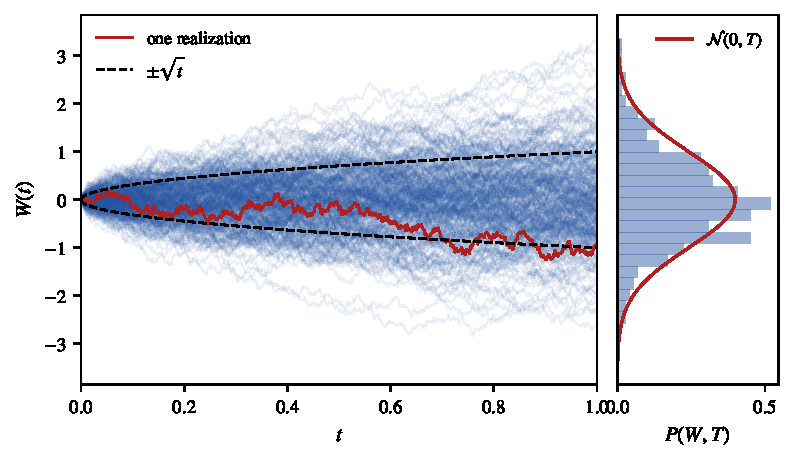
\includegraphics[width=0.9\textwidth]{images/wiener_ensemble.pdf}
\caption{Monte Carlo simulation of $300$ Wiener trajectories ($dW=\varepsilon\sqrt{dt}$, $\varepsilon\sim\mathcal{N}(0,1)$), spreading as $\sqrt{t}$ (dashed envelope). Right: histogram of the endpoints $W(T)$ against the exact density $\mathcal{N}(0,T)$. Generated by \texttt{images/code\_for\_images/wiener\_ensemble.py}.}
\label{fig:wiener-sim}
\end{figure}

\subsection{Arithmetic Brownian motion (Bachelier)}

Adding a constant drift produces the \emph{generalized Wiener process}, or arithmetic (additive) Brownian motion, with It\^o SDE\cite{Bachelier1900}
\begin{equation}
dx(t) = a\,dt + b\,dW(t),\qquad b\in\mathbb{R}^+,\ a\in\mathbb{R},
\end{equation}
called additive because the increments add up iteratively.
Integrating and taking moments exactly as before,
\begin{equation}
\mathbb{E}[x(t)] = a\,t \ \Longrightarrow\ a\ \text{is the drift},\qquad
\mathbb{E}[x^2(t)] = a^2 t^2 + b^2 t \ \Longrightarrow\ \mathrm{Var}[x(t)] = b^2 t,
\end{equation}
with standard deviation $\mathrm{s.d.}[x(t)] = b\sqrt{t}$ --- the quantity that finance calls the \emph{volatility} --- and the full distribution is Gaussian at all times,
\begin{equation}
\mathrm{PDF}(x,t) = \mathcal{N}(a\,t,\ b^2 t).
\end{equation}
A sample path is sketched in Figure~\ref{fig:abm}: the trajectory rattles around the straight line $\langle x(t)\rangle = a\,t$, with excursions that grow like $\sqrt{t}$.

\begin{figure}[h!]
\centering
\begin{tikzpicture}[scale=1.0]
  \draw[->] (-0.2,0) -- (7.2,0) node[right]{$t$};
  \draw[->] (0,-1.0) -- (0,2.6) node[above]{$x(t)$};
  % mean line <x(t)> = a t
  \draw[dashed,thick] (0,0) -- (6.8,2.2) node[right]{$\langle x(t)\rangle = a\,t$};
  % a jagged sample path fluctuating around the mean
  \draw[thick,blue!60!black] (0,0)
     -- (0.4,0.25) -- (0.8,0.05) -- (1.2,0.5) -- (1.6,0.35) -- (2.0,0.8)
     -- (2.4,0.55) -- (2.8,1.05) -- (3.2,0.8) -- (3.6,1.25) -- (4.0,1.0)
     -- (4.4,1.55) -- (4.8,1.3) -- (5.2,1.8) -- (5.6,1.55) -- (6.0,2.1)
     -- (6.4,1.85) -- (6.8,2.35);
\end{tikzpicture}
\caption{Arithmetic Brownian motion: a sample path fluctuating around the linear mean $\langle x(t)\rangle = a\,t$.}
\label{fig:abm}
\end{figure}

This was, in fact, the very first mathematical model of stock prices, proposed by Bachelier in his 1900 thesis\cite{Bachelier1900} --- five years before Einstein's paper on Brownian motion.
Historically glorious, but as a price model it has a fatal flaw: since the Gaussian has unbounded support and the fluctuations grow in probability, there is a nonzero probability that the price becomes \emph{negative}, which is not admissible for a stock.
Its autocovariance, for the record, is
\begin{equation}
\mathrm{Cov}[x(t),x(s)] = \mathbb{E}[x(t)x(s)] - \mathbb{E}[x(t)]\mathbb{E}[x(s)] = b^2\langle W(t)W(s)\rangle = b^2\min(t,s).
\end{equation}
Note that so far we have not needed It\^o's formula at all: with constant coefficients, everything is linear.
The next example is where the new calculus earns its keep.

\subsection{Multiplicative linear noise}

Consider now an It\^o process in which the noise enters \emph{multiplicatively}, proportional to the process itself,
\begin{equation}
dx(t) = b\,x(t)\,dW(t) \ \Longrightarrow\ \frac{dx(t)}{x(t)} = b\,dW(t) \ne d\ln x(t),
\end{equation}
and the inequality on the right is the whole point: in ordinary calculus $dx/x$ \emph{would} equal $d\ln x$, but here it does not, and It\^o's formula tells us by how much it fails.
Take $f(x)=\ln x$ (with $x(0)>0$); applying~\eqref{eq:ito-formula} with $a=0$, $\partial_x f = 1/x$ and $\partial_x^2 f = -1/x^2$,
\begin{equation}
d\ln x(t) = \left[\,0\cdot\frac{1}{x} + \frac{1}{2}b^2 x^2\left(-\frac{1}{x^2}\right)\right]dt + b\,x\,\frac{1}{x}\,dW(t) = -\frac{b^2}{2}\,dt + b\,dW(t).
\end{equation}
The anomalous term has generated a \emph{negative drift} $-b^2/2$ out of pure noise.
In logarithmic variables the process is now simple --- an additive Brownian motion --- with
\begin{equation}
\mathbb{E}[\ln x(t)] = \ln x_0 - \frac{b^2}{2}\,t,\qquad \mathrm{Var}[\ln x(t)] = b^2 t.
\end{equation}
Integrating and exponentiating back,
\begin{equation}
\ln x(t) = \ln x(0) - \frac{b^2}{2}\,t + b\,W(t) \ \Longrightarrow\ x(t) = x_0\,\exp\!\left\{-\frac{b^2}{2}\,t + b\,W(t)\right\},
\end{equation}
which is manifestly positive at all times.
One more check is instructive.
Setting $z=\ln x(t)\sim\mathcal{N}\!\big(\ln x_0-\tfrac{b^2}{2}t,\,b^2 t\big)$ and using the Gaussian identity $\langle e^{z}\rangle = e^{\langle z\rangle + \frac{1}{2}\mathrm{Var}[z]}$,
\begin{equation}\begin{split}
\mathbb{E}[x(t)] = \langle e^{z}\rangle &= e^{\,\langle z\rangle + \frac{1}{2}\mathrm{Var}[z]}\\
&= e^{\ln x_0 - \frac{b^2}{2}t}\,e^{\frac{b^2}{2}t} = x_0.
\end{split}\end{equation}
The two effects cancel exactly: the anomalous drift pushes the \emph{typical} trajectory down, while the fat upper tail of the exponential pulls the \emph{mean} up, and the mean is preserved despite the multiplicative noise.
This tug-of-war between median and mean is a recurring theme in finance.

\paragraph*{Geometric Brownian motion.}

Adding a linear drift to the multiplicative noise gives the \emph{geometric Brownian motion} (GBM), with It\^o SDE
\begin{equation}
dx(t) = a\,x(t)\,dt + b\,x(t)\,dW(t),\qquad b>0,\ a\in\mathbb{R},
\end{equation}
which is best read after dividing by $x$: the \emph{percentage} change $\dfrac{dx(t)}{x(t)} = a\,dt + b\,dW(t)$ is an arithmetic Brownian motion.
Percentage changes, not absolute ones, are what investors actually care about --- a 1\,\euro{} move means something very different for a 10\,\euro{} stock and a 1000\,\euro{} one --- and this is the economic rationale for the multiplicative structure.
By It\^o's formula, exactly as in the previous subsection but keeping the drift,
\begin{equation}
d\ln x(t) = \left(a - \frac{b^2}{2}\right)dt + b\,dW(t),
\end{equation}
so the increments $\ln\!\big(x(t+dt)/x(t)\big)$ --- the \emph{log-returns} --- are Gaussian, and the arithmetic Brownian motion of the logarithm becomes the geometric motion of the price.
As before,
\begin{equation}
\mathbb{E}[\ln x(t)] = \ln x(0) + \left(a-\frac{b^2}{2}\right)t,\qquad \mathrm{Var}[\ln x(t)] = b^2 t,
\end{equation}
\begin{equation}
\mathrm{PDF}(\ln x(t),t) = \mathcal{N}\!\left(\ln x_0 + \Big(a-\frac{b^2}{2}\Big)t,\ b^2 t\right),
\end{equation}
and translating back to the price itself,
\begin{equation}
\mathbb{E}[x(t)] = x_0\,e^{at},\qquad \mathrm{Var}[x(t)] = x_0^2\,e^{2at}\big(e^{b^2 t}-1\big).
\end{equation}
The process never becomes negative and its mean grows exponentially at rate $a$, which makes GBM a \emph{plausible model for spot prices} --- indeed, the standard one, as we will see at length in the next chapter.
It was introduced in finance by Osborne in 1959\cite{Osborne1959}, and was later given a proper economic rationale by Samuelson (1965)\cite{Samuelson1965}.
% CLAUDE NOTE: the notes cite "Samuelson 1960"; corrected to 1965 in the text at the
% author's request (2026-07-02). The reference is Samuelson's "Rational Theory of
% Warrant Pricing", Industrial Management Review 6 (1965).
Since the model is Markovian, the prices before $x(0)$ are irrelevant to the future --- an assumption still debated, to which we return in Chapter~5.

\subsection{The Ornstein--Uhlenbeck process}

Our last and richest example is the \emph{Ornstein--Uhlenbeck} (OU) process.
It occupies a special place in the theory: by \emph{Doob's theorem}\cite{Doob1942,UhlenbeckOrnstein1930} under the usual nondegeneracy and regularity assumptions it characterizes the stationary scalar Gaussian Markov case (in the strong sense, $P_t(x,t)=P_t(x)$).
Uniqueness makes it the default model for any quantity that fluctuates around a stable level: short-term interest rates, volatility, or the velocity of a Brownian particle.
Its It\^o SDE is
\begin{equation}
dx(t) = -\kappa\,x\,dt + \sqrt{D}\,dW(t),\qquad \kappa>0,\ [\kappa]=T^{-1},\ \tau=\frac{1}{\kappa},
\end{equation}
a random walk tethered by a linear restoring force: whenever $x$ wanders away from zero, the drift $-\kappa x$ pulls it back, on the characteristic time scale $\tau=1/\kappa$.

To solve it we use the substitution $f(x,t)=x\,e^{\kappa t}$ (an integrating factor), designed precisely to absorb the restoring drift.
By It\^o's formula,
\begin{equation}
df(x,t) = \left[\frac{\partial f}{\partial t} + a\frac{\partial f}{\partial x} + \frac{1}{2}b^2\frac{\partial^2 f}{\partial x^2}\right]dt + b\frac{\partial f}{\partial x}\,dW(t) = \sqrt{D}\,e^{\kappa t}\,dW(t),
\end{equation}
because the two drift contributions cancel identically ($\kappa x e^{\kappa t} - \kappa x e^{\kappa t}=0$) and $f$ is linear in $x$, so no anomalous term appears.
What remains is a pure (time-modulated) noise, which we integrate at sight:
\begin{equation}
\int_0^t df(x(t'),t') = \sqrt{D}\int_0^t e^{\kappa t'}\,dW(t'),
\end{equation}
and since $x(t)=f\,e^{-\kappa t}$ with $x(0)$ almost surely fixed,
\begin{equation}
x(t) = x_0\,e^{-\kappa t} + \sqrt{D}\int_0^t e^{-\kappa(t-t')}\,dW(t').
\end{equation}
The structure is transparent: the initial condition decays exponentially, while the noise accumulates --- but each past kick $dW(t')$ is remembered only with the fading weight $e^{-\kappa(t-t')}$.
Taking the mean (the It\^o integral averages to zero),
\begin{equation}
\mathbb{E}[x(t)] = x_0\,e^{-\kappa t},
\end{equation}
and, computing the variance with the It\^o isometry,
\begin{equation}\begin{split}
\mathrm{Var}[x(t)] = \Big\langle\big(x(t)-\langle x(t)\rangle\big)^2\Big\rangle &= D\,e^{-2\kappa t}\int_0^t \big(e^{\kappa t'}\big)^2\,dt'\\
&= D\,e^{-2\kappa t}\,\frac{e^{2\kappa t}-1}{2\kappa} = \frac{D}{2\kappa}\big(1-e^{-2\kappa t}\big).
\end{split}\end{equation}

The two limiting regimes are revealing.
For long times, $t\gg1/\kappa$, the memory of the initial condition is gone and the variance saturates,
\begin{equation}
\mathbb{E}[x(t)]\to0,\qquad \mathrm{Var}[x(t)]\to\frac{D}{2\kappa},
\end{equation}
so the distribution converges to a stationary law; a process initialized with fixed $x_0$ is not stationary at finite times: the injection of noise ($D$) and the dissipation of the restoring force ($\kappa$) balance.
For short times, $t\ll1/\kappa$, expanding the exponentials gives
\begin{equation}
\mathbb{E}[x(t)]\to x_0\{1-\kappa t+\dots\},\qquad \mathrm{Var}[x(t)]\to\frac{D}{2\kappa}\{1-1+2\kappa t+\dots\} = D\,t,
\end{equation}
i.e.\ before the restoring force has had time to act, the process simply \emph{diffuses} like a free Brownian motion.
The full distribution at all times is Gaussian,
\begin{equation}
\mathcal{N}\!\left(x_0\,e^{-\kappa t},\ \frac{D}{2\kappa}\big[1-e^{-2\kappa t}\big]\right) \xrightarrow{\ t\to\infty\ } \mathcal{N}\!\left(0,\ \frac{D}{2\kappa}\right) = P^{\mathrm{O.U.}}(x).
\end{equation}
In the original physical setting, where $x$ is the velocity of a Brownian particle, the stationary law $P^{\mathrm{O.U.}}(v) = P^{\mathrm{M.B.}}(v)$ is nothing but the Maxwell--Boltzmann distribution: the OU process describes, in real time, how an out-of-equilibrium velocity distribution relaxes to thermal equilibrium, and matching the two stationary variances yields the Einstein fluctuation--dissipation relation, $D/(2\kappa)=k_BT/m$ for the velocity process.
Figure~\ref{fig:ou} sketches the characteristic noisy relaxation of a single path, and Figure~\ref{fig:ou-sim} shows the full Monte Carlo picture: an ensemble of paths hugging the analytic mean, with the fluctuation band saturating at $\pm\sqrt{D/2\kappa}$.

\begin{figure}[h!]
\centering
\begin{tikzpicture}[scale=1.0]
  \draw[->] (-0.2,0.5) -- (7.2,0.5) node[right]{$t$};
  \draw[->] (0,-0.4) -- (0,2.6) node[above]{$x(t)$};
  \node[left] at (0,2.1) {$x_0$};
  % equilibrium mean level
  \node[left] at (0,0.5) {$0$};
  % damped, noisy relaxation toward the level
  \draw[thick,red!60!black] (0,2.1)
    -- (0.4,1.7) -- (0.8,1.9) -- (1.2,1.4) -- (1.6,1.55) -- (2.0,1.1)
    -- (2.4,1.25) -- (2.8,0.85) -- (3.2,1.0) -- (3.6,0.7) -- (4.0,0.8)
    -- (4.4,0.55) -- (4.8,0.65) -- (5.2,0.5) -- (5.6,0.6) -- (6.0,0.45)
    -- (6.4,0.55) -- (6.8,0.5);
\end{tikzpicture}
\caption{Ornstein--Uhlenbeck process: a noisy, exponentially damped relaxation of $x(t)$ from $x_0$ towards the stationary level, with asymptotic variance $D/2\kappa$.}
\label{fig:ou}
\end{figure}

% Figure generated from raw notes page 9 by images/code_for_images/ou_ensemble.py
\begin{figure}[h!]
\centering
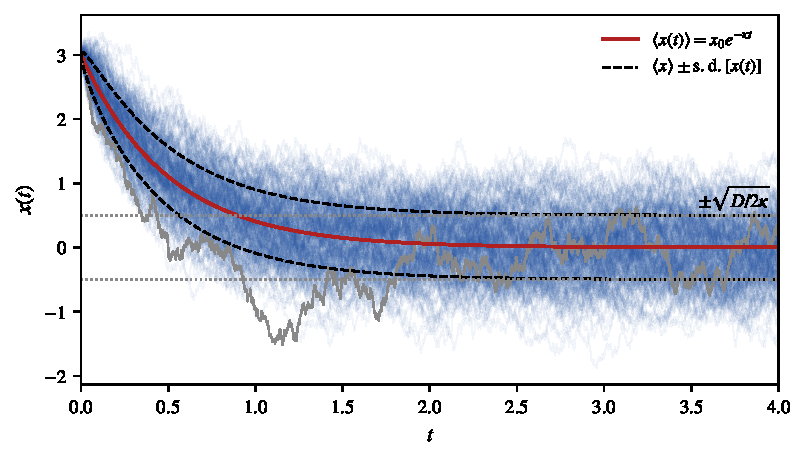
\includegraphics[width=0.9\textwidth]{images/ou_ensemble.pdf}
\caption{Monte Carlo simulation of $200$ Ornstein--Uhlenbeck paths ($\kappa=2$, $D=1$, $x_0=3$), relaxing from the common initial condition to the stationary band. The red curve is the analytic mean $x_0e^{-\kappa t}$; the dashed curves are the $\pm1$ standard-deviation envelope, saturating at $\pm\sqrt{D/2\kappa}$ (dotted). Generated by \texttt{images/code\_for\_images/ou\_ensemble.py}.}
\label{fig:ou-sim}
\end{figure}

With the Wiener process, geometric Brownian motion, and the Ornstein--Uhlenbeck process in hand, our toolbox is complete.
The next chapter puts it to work on the problem that made stochastic calculus famous: the fair pricing of financial derivatives.


\chapter{Financial Derivatives and Pricing}

The machinery of stochastic processes and stochastic calculus developed in the previous chapters finds its most celebrated application in the theory of \emph{financial derivatives}.
The problem it solves is easy to state and was, for most of a century, believed to have no objective answer: what is the \emph{fair price} of a contract whose value depends on the unknown future price of something else?
This chapter builds the answer from the ground up.
We first describe the structure of financial markets and the main asset classes; we then introduce options and the no-arbitrage principle; and we finally derive the Black--Scholes equation and solve it, obtaining the formula that in 1973 turned derivative pricing from an art into a science.


\section{Financial markets}

A \emph{financial market} is a physical or virtual venue in which agents exchange \emph{assets} at a \emph{spot price} (instantaneous price) $S(t)$, determined by the law of supply and demand.
The participants are heterogeneous --- banks, hedge funds, brokers, individual traders --- and so are the venues.
\emph{Stock markets} in particular come in three flavours: the \emph{official exchanges} (NYSE, LSE, \ldots), of which there are about $200$ worldwide, historically paper-based; the fully \emph{electronic} exchanges (Nasdaq, Euronext, \ldots), where trading is algorithmic; and \emph{hybrid} venues such as today's NYSE, which combine both.
Alongside the official markets there exist non-official ones, distinguished by the absence of intermediaries.

% CLAUDE NOTE: the following two paragraphs of background for readers new to finance
% were added at the author's request (2026-07-06); they expand the prose without
% altering any of the notes' content.
Since this book is written for physicists, it is worth pausing on how a trade actually happens, because the microscopic mechanism is what gives the spot price its meaning.
At any instant, an exchange maintains for each asset an \emph{order book}: a list of offers to buy at stated prices (the \emph{bids}) and offers to sell at stated prices (the \emph{asks}).
The highest bid and the lowest ask face each other across a small gap, the \emph{bid--ask spread}; a trade occurs when someone accepts the best price on the opposite side, and the price at which this happens is the quoted price of the asset.
The market is called \emph{liquid} when the book is thick --- when there are so many standing offers that one can buy or sell a large quantity at any moment without moving the price appreciably.
Liquidity is the market's analogue of a good thermal bath: it is what allows a single agent to exchange with the collective without perturbing it, and most of the idealizations of this chapter (continuous trading, negligible spread) are statements about high liquidity.

Two more pieces of jargon will recur.
An investor is \emph{long} an asset after buying it, profiting if the price rises; and is \emph{short} after selling an asset it does not own --- borrowing it, selling it, and planning to buy it back later --- profiting if the price falls.
Short selling looks exotic but is essential: it is what allows negative positions, and therefore hedges, to exist; we will meet a short position at the heart of the Black--Scholes argument.

The central object of the theory is the spot price, and two of its properties deserve to be stated explicitly.
First, the spot price is \emph{unique}: at any given time there is a single price in the whole market --- there is no ``price here'' and ``price there''.
(Why this is so is a question we defer for a few pages; the answer is arbitrage.)
Second, it is a price of \emph{equilibrium}: it arises from the matching of supply and demand, i.e.\ from the meeting of the best ask and the best bid, with a bid--ask spread $\Delta(\text{ask},\,\text{bid})\to 0$.
In reality $\Delta>0$, because of transaction costs and related frictions, but the idealization is a good one for liquid markets.

Under what conditions does such an equilibrium price exist at all?
The classical answer requires the market to be \emph{atomistic} --- no single agent has a large influence --- and to satisfy three structural conditions.
There must be \emph{perfect competition and information}: entry and exit are free, and all participants know everything, instantly.
There must be \emph{no arbitrage}: no free profits exist, and any asymmetry of information is resolved immediately.
And the market must be \emph{complete}: the assets already present span the entire space of probabilities, so that the payoff of any new asset can be replicated with existing ones.
When these conditions hold, the \emph{Arrow--Debreu} model applies, and one can prove that a system of equilibrium prices exists.
In such a market the gain available to an investor is the \emph{interest rate}, plus a premium for bearing \emph{risk} --- a decomposition that will guide us throughout this chapter.


\section{Risk and the Efficient Market Hypothesis}

\subsection{Types of risk}

Since risk is what one is paid to bear, we should say what kinds there are.
Financial risk is traditionally classified into three categories.
\emph{Operational risk} covers human errors, computer crashes, and similar accidents of implementation --- a category whose weight has grown with automation: today some $60$--$75\%$ of all transactions worldwide are executed by algorithmic trading, much of it speculative high-frequency trading.
% CLAUDE NOTE: the algorithmic-trading figure is from the course slides
% (Mercati & Strumenti Finanziari), added 2026-07-06.
\emph{Credit risk} is the risk that the counterparty does not honour the obligations of the contract --- the risk of insolvency.
\emph{Market risk}, finally, is the one that will concern us: the random fluctuation of prices themselves, caused partly by the internal dynamics of supply and demand, partly by exogenous factors (politics, disasters, \ldots), and partly by psychological factors --- imitation, panic --- whose study belongs to \emph{behavioural economics}.
The Black--Scholes theory we develop below deals with market risk only; credit risk is assumed away, an assumption whose limits became painfully visible in 2008.

\subsection{The Efficient Market Hypothesis}

The fundamental question, on which the applicability of everything we have built so far depends, is this:

\medskip
\begin{center}
\emph{Is the dynamics of an asset a Markov process?}
\end{center}
\medskip

Figure~\ref{fig:djia} shows why the question is not rhetorical: the trajectory of a major index looks like the noisy paths of the previous chapters, but it visibly responds to identifiable exogenous shocks --- trade disputes, a pandemic, central-bank decisions --- and one may legitimately ask whether such a history can be modelled by a memoryless It\^o SDE driven by market risk alone.

% Figure after the course slides (Mercati & Strumenti Finanziari);
% generated by images/code_for_images/djia_events.py from FRED series DJIA.
\begin{figure}[h!]
\centering
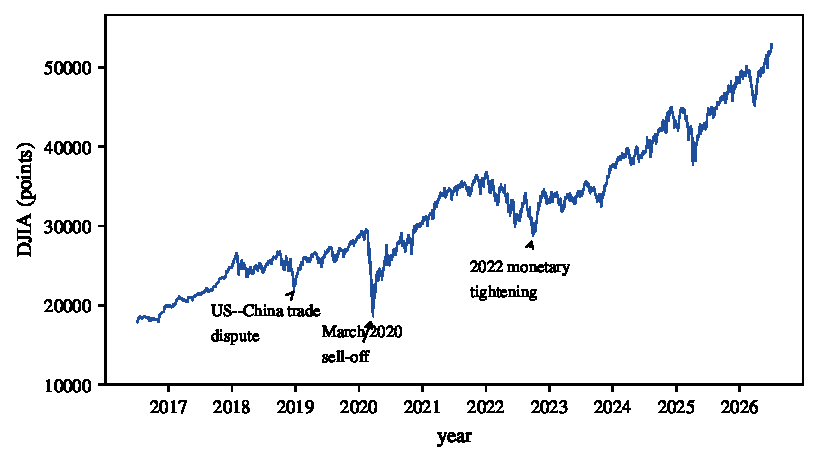
\includegraphics[width=0.9\textwidth]{images/djia_events.pdf}
\caption{The Dow Jones Industrial Average, daily closes 2016--2026 (FRED series DJIA), with some major exogenous events annotated. The fundamental question of this section: can this dynamics be modelled as a Markov process? Generated by \texttt{images/code\_for\_images/djia\_events.py}.}
\label{fig:djia}
\end{figure}

If prices carry memory, the Fokker--Planck machinery of Chapter~3 does not apply, and neither do the SDE models of Chapter~4.
The Markov property holds only if the \emph{Efficient Market Hypothesis} (EMH) does.
The EMH, formulated by Fama in 1970\cite{Fama1970}, states that the market reflects fully and instantaneously all available information: whatever can be known about an asset is already incorporated in its current price.
If this is true, the past adds nothing to the present --- which is precisely the Markov property.
The hypothesis carries several implications: information must be instantly and freely available to all agents (only the present matters); the market must be \emph{liquid}, so that anyone can buy and sell easily; and transaction costs must be negligible.
Assembling the pieces, we can summarize the structural assumptions of this chapter in a single line:
\begin{equation}
\text{EMH} + \text{no arbitrage} + \text{completeness} \;=\; \text{Arrow--Debreu}.
\end{equation}
The EMH is the hypothesis that mathematical finance later made rigorous in the fundamental theorems of asset pricing (Section~\ref{sec:rn-girsanov}); and if the market is efficient, the economically rational standard model for asset prices is Samuelson's geometric Brownian motion --- work recognized with the 1970 Nobel Prize in Economics.
% CLAUDE NOTE: the FTAP remark and the Samuelson Nobel mention follow the course slides
% (Mercati & Strumenti Finanziari), added 2026-07-06.
Whether real markets satisfy the EMH is an empirical question --- and the answer, as we shall see in Section~\ref{sec:gbm-limits} and again in Chapter~7, is ``only approximately''.


\section{Financial assets}

Before specializing to derivatives, it is worth surveying what is actually traded.
The main asset classes are the following.
\begin{itemize}
    \item \textbf{Currencies}: money itself, traded against other money.
    \item \textbf{Commodities}: energy, precious metals, agricultural products, and so on.
    \item \textbf{Stocks} (equities): securities issued by a company to raise capital by selling a fraction of its ownership, without any obligation of repayment.
    For the buyer they offer visibility, a voice in company decisions, and possible dividends.
    A \emph{stock index} is the average (arithmetic or weighted) value of a group of equity titles --- the S\&P\,500, which averages five hundred large American companies weighted by capitalization, will reappear several times in this book; other examples are the Dow Jones (USA), the FTSE\,100 (UK), the CAC\,40 (France), the DAX (Germany), the FTSE\,MIB (Italy), and the Nikkei (Japan).
    % CLAUDE NOTE: index examples from the course slides, added 2026-07-06.
    \item \textbf{Bonds} (obligations): debt securities issued by states or companies to raise large sums; they have a \emph{maturity} $T$ at which the capital is repaid with interest, and are comparatively low-risk.
    They are the subject of Chapter~6.
    \item \textbf{Derivatives}: contracts whose value derives from other assets --- the subject of the present chapter.
    \item \textbf{Cryptocurrencies}: assets living outside the official markets.
\end{itemize}
Portfolios mixing these classes (gold, currencies, stocks, bonds, ETFs\ldots) are the standard tool of diversification and, in general, of speculation.
A \emph{portfolio} is simply a weighted collection of assets held together, and \emph{diversification} --- not putting all the eggs in one basket --- has a rationale a physicist will recognize at once: if the fluctuations of $N$ assets were independent, the relative fluctuation of their sum would shrink as $1/\sqrt{N}$, exactly like the relative energy fluctuations of $N$ weakly coupled subsystems.
Mixing imperfectly correlated assets therefore reduces risk at no cost in average return; the catch, to which we return in Chapter~7, is that in a crisis the correlations rise and the $\sqrt{N}$ protection evaporates precisely when it is needed.
% CLAUDE NOTE: the diversification paragraph was added for readers new to finance at the
% author's request (2026-07-06).
To appreciate the scale of all this: the total value of global financial assets is approximately \$461 trillion, against a world GDP of roughly \$100 trillion.
Finance is not a small correction to the real economy; by market value it is several times larger.


\section{Derivatives and options}

A \emph{derivative} is a contract between a buyer and a seller whose value \emph{derives} from the value of other financial instruments (currencies, stocks, etc.).
The idea is old: derivatives appeared in the Netherlands in the 1600s for the tulip trade, and the first recorded example is usually attributed to Aristotle (\emph{Politics} I.xi), where Thales, expecting a good olive harvest, secured in advance the right to use the local olive presses.
Then as now, derivatives serve two purposes: \emph{hedging}, i.e.\ insurance against unfavourable price movements, and \emph{speculation}, i.e.\ profiting from anticipated ones.

One important type of derivative is the (\emph{stock}) \textbf{option}.
An option is a contract between two parties --- the \textbf{writer}, who sells the contract, and the \textbf{holder}, who buys it --- granting the holder the right, but not the obligation, to buy (\textbf{call}) or sell (\textbf{put}) from/to the writer the \emph{underlying asset} (the stock) at a fixed price $X$, the \emph{strike}, at a future time $T$, the \emph{maturity}.

The contract is fundamentally \emph{asymmetric}, and the asymmetry is what makes pricing non-trivial.
The holder may exercise the option or walk away, at will; the writer, if the holder exercises, \emph{must} sell (or buy) at the agreed price, whatever the market is doing.
The holder buys optionality; the writer sells certainty and takes on risk.

Options come in various types.
\emph{European} options are exercisable only at maturity $T$; within this family live the \emph{plain vanilla} options, but also asiatic options, barrier options, and other so-called exotics.
\emph{American} options are exercisable at any time $t\le T$, a freedom that complicates the analysis considerably; we will be able to price them only numerically, in Section~\ref{sec:crr}.


\section{Option payoffs and fair pricing}

We can now state the problem of the chapter.
The \emph{option pricing problem} is to find the unique fair (equilibrium) price $O(S,t)$ of the contract at the moment of signing --- fair in the sense that neither party makes a riskless profit at the expense of the other, at any $t\le T$:
\begin{equation}
O(S,t) = C_{\text{BS}}(S,t) \quad \forall\, t \le T.
\end{equation}
Solving this problem is the achievement of Black and Scholes; before getting there, we need to understand what an option is worth in the one situation where no theory is required, namely \emph{at maturity}.

\subsection{Call option}

Consider first the hedging use of a call, and let us put numbers on it, because the insurance logic is easiest to absorb on a concrete case.
% CLAUDE NOTE: the numerical example was added for readers new to finance at the
% author's request (2026-07-06); the underlying scenario (the gas-consuming company)
% is the one in the handwritten notes.
Suppose the holder runs a large energy company that consumes gas, currently at $90$\,\euro{} per unit, and fears that the price will slip upwards over the next year; buying a call option at strike $X = 100$\,\euro{}, for a premium of, say, $5$\,\euro{}, insures against exactly this.
If at maturity gas trades at $130$\,\euro{}, the company exercises and buys at $100$: the insurance has capped its cost at $105$\,\euro{} per unit (strike plus premium) instead of $130$.
If instead gas trades at $80$\,\euro{}, the company simply buys on the market and lets the option expire: the premium of $5$\,\euro{} is the cost of the peace of mind, exactly like an unused fire-insurance policy.
In general, at maturity $T$ two scenarios are possible.
\begin{enumerate}[label=\alph*)]
    \item If $S(T) < X$, buying at the market price is cheaper than exercising; the holder does not exercise, and simply loses the premium paid for the option --- an insurance policy that turned out not to be needed.
    \item If $S(T) > X$, the holder exercises, buys at $X$ what the market values at $S(T)$, and gains $S(T)-X$.
\end{enumerate}
For purely speculative purposes the same logic applies, with the asset sold immediately after exercise: if $S(T)>X$ the speculator pockets a guaranteed $S_T - X$ (minus the premium, of course).

Both scenarios are summarized by the \textbf{payoff} of the call,
\begin{equation}\label{eq:call-payoff}
C(S_T, T) = \begin{cases} S_T - X & \text{if } S_T > X, \\ 0 & \text{if } S_T \le X, \end{cases} = \max\{S_T - X,\, 0\} = \{S_T - X\}_+,
\end{equation}
the ``hockey-stick'' function of Figure~\ref{fig:call-payoff}: flat at zero below the strike, rising with unit slope above it.

\begin{figure}[h!]
\centering
\begin{tikzpicture}
    \draw[->] (0,0) -- (5,0) node[right] {$S_T$};
    \draw[->] (0,0) -- (0,3) node[above] {$C(S_T,T)$};
    \draw[thick, blue] (0,0) -- (2.5,0);
    \draw[thick, blue] (2.5,0) -- (4.5,2);
    \node[below] at (2.5,0) {$X$};
\end{tikzpicture}
\caption{Payoff of a European call at maturity: worthless below the strike $X$, linear in $S_T$ above it.}
\label{fig:call-payoff}
\end{figure}

The payoff tells us what the option is worth at $T$; the problem, of course, is that we would like to know its value \emph{now}.

\subsection{Put option}

A put is the mirror image: a bet on a price \emph{decrease}.
The holder expects the asset to lose value and secures the right to sell it at $X > S_T$, gaining $X - S_T$ if the fall indeed materializes; if instead $S_T \ge X$ the right is worthless, since selling at the market price is better.
The \textbf{payoff} of the put is therefore
\begin{equation}\label{eq:put-payoff}
P(S_T, T) = \begin{cases} X - S_T & \text{if } S_T < X, \\ 0 & \text{if } S_T \ge X, \end{cases} = \max\{X - S_T,\, 0\} = \{X - S_T\}_+,
\end{equation}
the reflected hockey stick of Figure~\ref{fig:put-payoff}.

\begin{figure}[h!]
\centering
\begin{tikzpicture}
    \draw[->] (0,0) -- (5,0) node[right] {$S_T$};
    \draw[->] (0,0) -- (0,3) node[above] {$P(S_T,T)$};
    \draw[thick, red] (0,2.5) -- (2.5,0);
    \draw[thick, red] (2.5,0) -- (4.5,0);
    \node[below] at (2.5,0) {$X$};
\end{tikzpicture}
\caption{Payoff of a European put at maturity: linear below the strike, worthless above it.}
\label{fig:put-payoff}
\end{figure}

A caveat: these clean payoff formulas hold only for \emph{plain vanilla} options, which depend solely on $T$ and on the terminal price $S_T$.
For \emph{exotic} options the payoff involves the whole price history; in the \emph{asiatic} case, for instance, it depends on the average of the prices during the life of the contract,
\begin{equation}
\max\!\Bigl\{\frac{1}{n}\sum_{i=1}^{n}S_{t_i} - X,\, 0\Bigr\},
\end{equation}
and for such contracts no closed formula exists --- one resorts to numerical (Monte Carlo) simulations.

\subsection{The no-arbitrage argument}

The terminal price $S_T$ is a stochastic process --- but which one, and priced how?
We will model it with the geometric Brownian motion of Chapter~4; but before any model, a purely logical argument already pins down the value of the option \emph{at maturity}.
Follow the money:
\begin{enumerate}
    \item the holder $H$ exercises the option and acquires the stock at $X$ at time $T$;
    \item the writer $W$ is obligated to sell at $X$;
    \item $W$ observes that $S_T > X$ and buys the stock in the market, selling it immediately to $H$; the round trip costs $W$ exactly $S_T - X$.
\end{enumerate}
For neither party to be robbed, the price of the option at maturity must satisfy $X + C(S_T) = S_T$, i.e.\ $C(S_T)=S_T-X$; any other value would create an instantaneous riskless profit --- an \emph{arbitrage} --- for one of the two parties, and would be arbitraged away immediately.
To avoid being at a disadvantage in the future, then, the parties can already agree that at maturity $C(S_T) = S_T - X$ is the fair value.

The real problem is to propagate this terminal value \emph{backwards}: the fair value in the present must be deduced from the future.
One models the future between $t=0$ and $t=T$ with a stochastic process, and this is where the GBM enters.
The GBM was introduced as a price model by Osborne in 1959\cite{Osborne1959} and applied to economics in 1965, notably by Samuelson\cite{Samuelson1965}.
% CLAUDE NOTE: The notes write "1960" for Samuelson; corrected to 1965 in the text at the
% author's request (2026-07-02). The canonical reference is Samuelson (1965).
The older Bachelier model (arithmetic Brownian motion, Chapter~4) is ruled out for the reason we found there: it assigns positive probability to negative prices, which is unphysical.


\section{The risk-free rate and the bank account}\label{sec:bank-account}

To understand why the GBM is the right model, let us first understand the alternative to investing at all: the bank.
Consider a \emph{bank account}: the agent starts outside the market, with money in the bank, at $t_0 = 0$ with capital $S(t_0)=S_0$.
The bank pays a risk-free interest rate $r$, assumed constant, so that with \emph{simple interest}
\begin{equation}
S_t := S(t) = S_0 + S_0\, r\, t \qquad \forall\, t.
\end{equation}
The rate $r$ represents the cost (or reward) of money over time: a euro today is worth more than a euro tomorrow, and $r$ measures by how much.

Simple interest, however, undercounts: nothing prevents the agent from cashing in at an intermediate time and reinvesting.
Splitting $[0,t]$ into $m$ steps of length $t/m$ and reinvesting the accrued interest at each step,
\begin{equation}
S_t = S_0\Bigl(1 + \frac{r\,t}{m}\Bigr)^m,
\end{equation}
and in the limit of continuous reinvestment, $m\to\infty$ (with $r$ small, so that $r\,t\ll 1$),
\begin{equation}
S_t \longrightarrow S_0\, e^{r\,t},
\end{equation}
which is \emph{compound interest in the continuum} --- sometimes called mathematical interest.
Exponential growth at rate $r$ is thus the baseline against which every investment must be measured.

The adjective \emph{risk-free} deserves a comment.
It means a guaranteed return with zero credit risk --- and it is, of course, an abstraction.
Even banks deemed ``too big to fail'' can fail, as the crisis of 2008 (and the state-financed rescues that followed) made clear; and the rate $r$ itself is not constant in time but fluctuates, following its own SDE $r(t)\to dr(t)$ with unknown future values --- the subject of Chapter~6.
Can one at least find a good \emph{proxy} for the ideal risk-free rate?
In practice, yes: the spot rate of AAA-rated government bonds (USA, Germany) with short maturity, between one and three months, whose default risk is negligible.
This identification gives the initial condition $dB_t = r\, B_t\, dt$ for the riskless asset, and hence, in the absence of risk,
\begin{equation}
dS_t = r\, S_t\, dt \quad\Longrightarrow\quad S_t = S_0\, e^{r\,t}.
\end{equation}


\section{Geometric Brownian Motion for stock prices}\label{sec:gbm-stocks}

Now let the agent leave the bank and enter the market; the risk is no longer zero, and the dynamics must say so.
Two ingredients are needed.

The first is the reward.
One introduces
\begin{equation}
\mu \;=\; \text{percentage return rate (historical rate of return)},
\end{equation}
a number extracted from real historical time series --- and \emph{not} universal: each asset has its own.
The deterministic part of the price dynamics becomes
\begin{equation}
dS_t = S_t\,\mu\, dt,
\end{equation}
formally identical to the bank account but with $\mu$ in place of $r$.
Why would anyone accept the risk unless $\mu > r$?
They would not: the return must exceed the risk-free rate, otherwise it would be more convenient to leave the money in the bank, and the excess $\mu - r$ is called the \emph{risk premium}.

The second ingredient is the risk itself.
By the EMH, information and transactions change the price instantaneously and unpredictably; this contributes a stochastic term $\sigma\, S_t\, dW_t$, where $\sigma$ is the \emph{historical volatility}, with the meaning of an instantaneous standard deviation.
Assembling the two pieces,
\begin{equation}\label{eq:gbm-sde}
dS_t = \mu\, S_t\, dt + \sigma\, S_t\, dW_t, \qquad \mu\in\mathbb{R},\; \sigma\in\mathbb{R}^+,
\end{equation}
which is precisely the SDE of \emph{Geometric Brownian Motion} (GBM), solved in Chapter~4.
The stock price, in this model, is a bank account whose interest rate has been made noisy.

\subsection{Log-returns}

The financially meaningful quantity is not the absolute change $dS_t$ but the \emph{percentage} return $dS_t/S_t$, which is adimensional --- it treats a 10\,\euro{} stock and a 1000\,\euro{} one on the same footing.
By It\^o's lemma applied to $\ln S_t$ (Chapter~4),
\begin{equation}
d\ln S_t = \Bigl(\mu\,\frac{S_t}{S_t}\frac{1}{S_t} - \frac{1}{2}\,\sigma^2\,\frac{S_t^2}{S_t^2}\frac{1}{S_t^2}\Bigr)\!dt + \sigma\,\frac{S_t}{S_t}\,\frac{1}{S_t}\,dW_t
= \Bigl(\mu - \frac{\sigma^2}{2}\Bigr)dt + \sigma\, dW_t,
\end{equation}
% CLAUDE NOTE: The notes write this via the Itô lemma with the generic partials;
% the above is the simplified final form: d ln S_t = (μ − σ²/2)dt + σ dW_t.
that is, $d\ln S_t = \frac{dS_t}{S_t} - \frac{1}{2}\sigma^2\,dt$: the log-return differs from the percentage return by the anomalous It\^o term.
These increments $d\ln S_t$ are the \emph{log-returns} (financial returns), and they are the quantities whose statistics one actually measures on market data.
Integrating,
\begin{equation}
\ln\frac{S_t}{S_0} = \bigl(\mu - \tfrac{\sigma^2}{2}\bigr)t + \sigma\, W_t
\quad\Longrightarrow\quad
S_t = S_0\,\exp\!\bigl\{\bigl(\mu-\tfrac{\sigma^2}{2}\bigr)t + \sigma\, W_t\bigr\} > 0,
\end{equation}
manifestly positive at all times, as a price should be.
It is immediate to verify that
\begin{equation}
\mathbb{E}\!\bigl[\ln\tfrac{S_t}{S_0}\bigr] = \bigl(\mu - \tfrac{\sigma^2}{2}\bigr)t, \qquad
\mathrm{Var}\!\bigl[\ln\tfrac{S_t}{S_0}\bigr] = \sigma^2 t,
\end{equation}
so the PDF of the log-returns is Gaussian --- a prediction we will test against reality, with instructive results, in Chapter~7.


\section{The log-normal distribution}\label{sec:log-normal}

If the log-returns are Gaussian, what is the distribution of the price itself?
One could attack the Fokker--Planck equation for $P(S,t \mid S_0,t_0)$ directly, but it is far more complicated than the one for $P(\ln S_t \mid \ln S_0, t_0)$, because $\ln S_t$ is the variable that diffuses Gaussianly; the smart move is to change variables in the probability density.

Let $P(\ln S_t \mid \ln S_0, t_0) := P(\ln S_t)$ be the Gaussian density of the logarithm; its normalization reads
\begin{equation}
\int_{-\infty}^{+\infty}\!d\ln S_t\; P(\ln S_t) = 1,
\qquad\text{with}\quad
d\ln S_t = \frac{dS_t}{S_t}
\end{equation}
(a normal change of variables --- no It\^o here, because we are integrating over values, not following a trajectory).
Since $\ln S_t \to +\infty$ when $S_t\to +\infty$ and $\ln S_t\to -\infty$ when $S_t\to 0$, the integration limits transform accordingly, and
\begin{equation}
\int_0^{+\infty}\!\frac{dS_t}{S_t}\; P(\ln S_t) = \int_0^{+\infty}\! dS_t\; P_{\ln}(S_t),
\end{equation}
where the density picks up a Jacobian factor $1/S_t$: this defines the \emph{log-normal probability density},
\begin{equation}\label{eq:log-normal}
P_{\ln}(S_t, t \mid S_0, t_0) = \frac{1}{S_t\sqrt{2\pi\sigma^2(t-t_0)}} \exp\!\biggl\{-\frac{\bigl[\ln\frac{S_t}{S_0} - (\mu-\frac{\sigma^2}{2})(t-t_0)\bigr]^2}{2\sigma^2(t-t_0)}\biggr\}.
\end{equation}
Note that the moments of $S_t$ can no longer be read off by inspection, as they could for a Gaussian; they must be computed.
Using the Gaussian identity $\langle e^z\rangle = e^{\langle z\rangle+\frac12\mathrm{Var}[z]}$ with $z=\ln S_t$, one finds
\begin{align}
\mathbb{E}[S_t] &= \int_0^{\infty}\!dS_t\; S_t\, P_{\ln}(S_t) = e^{\langle\ln S_t\rangle} \cdot e^{\frac{1}{2}\mathrm{Var}[\ln S_t]} = S_0\, e^{\mu(t-t_0)}, \label{eq:gbm-mean} \\[6pt]
\mathrm{Var}[S_t] &= e^{2\langle\ln S_t\rangle} \cdot e^{\mathrm{Var}[\ln S_t]}\bigl(e^{\mathrm{Var}[\ln S_t]}-1\bigr) = S_0^2\, e^{2\mu(t-t_0)}\bigl(e^{\sigma^2(t-t_0)}-1\bigr). \label{eq:gbm-var}
\end{align}
The mean grows exponentially at the full rate $\mu$ --- the $\sigma^2/2$ correction of the typical trajectory is compensated, as in Chapter~4, by the fat upper tail.

That fat tail is visible in the shape of the distribution, sketched in Figure~\ref{fig:lognormal}: the log-normal is skewed to the right, with the \emph{mode} to the left of the \emph{mean}.
The financial reading is worth remembering: most trajectories end up below the average (the mode is low), while a few end up far above it (the tail is long) --- high gains come with large risks.

\begin{figure}[h!]
\centering
\begin{tikzpicture}
    \draw[->] (0,0) -- (5.5,0) node[right] {$S_t$};
    \draw[->] (0,0) -- (0,3.2) node[above] {$P_{\ln}(S_t)$};
    \draw[thick, blue, domain=0.15:5, samples=100]
        plot (\x, {2.8*exp(-0.5*(ln(\x)-0.3)^2/0.25)/(\x*sqrt(2*3.14159*0.25))});
    \draw[dashed, gray] (0.95,0) -- (0.95,2.8) node[above, black, font=\footnotesize] {mode};
    \draw[dashed, gray] (1.55,0) -- (1.55,1.7) node[above, black, font=\footnotesize] {mean};
\end{tikzpicture}
\caption{The log-normal density of the price $S_t$: right-skewed, with the mode below the mean. Small gains are typical; large gains are rare but heavy.}
\label{fig:lognormal}
\end{figure}


\section{Limits of the GBM model}\label{sec:gbm-limits}

Before building an entire pricing theory on the GBM, intellectual honesty requires listing what is known to be wrong with it.
Three questions summarize the situation.
\begin{enumerate}
    \item \emph{Do prices really follow a Markov process?}
    This is equivalent to asking whether the EMH holds --- and the honest answer is: not really.
    Markets digest information quickly, but not instantaneously, and traces of memory remain.

    \item \emph{Is the distribution of log-returns Gaussian at every time scale?}
    That is, is
    \begin{equation}
    \mathrm{PDF}\!\Bigl[\ln\frac{S(t+\Delta t)}{S(t)}\Bigr] = \mathcal{N} \quad \forall\, t\ ?
    \end{equation}
    For $\Delta t$ of a month or longer the Gaussian is a fair description (this was Samuelson's defence of the model), but at high frequencies --- daily, and today down to seconds --- it fails visibly: the empirical distribution exhibits \emph{fat tails}, with extreme events far more probable than any Gaussian allows.
    Chapter~7 is devoted to this discrepancy.

    \item \emph{Is the volatility constant?}
    The model predicts $\mathrm{s.d.}[\ln r(\Delta t)] = \sigma\sqrt{\Delta t}$ with a fixed $\sigma$.
    The data say no: $\sigma$ itself depends on time (Engle), and quiet periods alternate with turbulent ones --- the phenomenon of \emph{volatility clustering}, also taken up in Chapter~7.
    % CLAUDE NOTE: the notes write "(Engls)"; the intended reference is Robert F. Engle,
    % whose ARCH models of time-varying volatility earned the 2003 Nobel Prize in Economics.
\end{enumerate}
One can generalize the model to address each failure, and Chapter~7 will do so; but every generalization must be solved numerically.
The GBM is the only model of its family that is analytically solvable, and this --- as much as its economic plausibility --- explains its enduring centrality.


\section{The Black--Scholes equation}\label{sec:black-scholes}

We now have all the ingredients: a model for the underlying (the GBM), a terminal condition (the payoff), and a guiding principle (no arbitrage).
The Black--Scholes model (Black \& Scholes, 1973; Merton, 1973)\cite{BlackScholes1973, Merton1973} assembles them into a partial differential equation for the option price --- work recognized with the 1997 Nobel Prize in Economics, awarded to Scholes and Merton.
Given the terminal payoff $C(S_T, t=T)=\{S_T-X\}_+$, the PDE propagates the value backwards and yields $C(S,t)$ for all $t\le T$.

\subsection{Model hypotheses}\label{sec:bs-hypotheses}

The derivation rests on seven hypotheses, which we number for later reference.
\begin{enumerate}[label=\roman*)]
    \item The only risk is \emph{market risk} (no credit risk); price fluctuations are driven by supply and demand.
    \item The \textbf{EMH} holds (Markov property), and the stock follows a GBM:
    \begin{equation}
    dS_t = \mu\, S_t\, dt + \sigma\, S_t\, dW_t.
    \end{equation}
    \item The volatility $\sigma$ is constant (relaxing this leads to models \`a la Eston), and the risk-free rate $r$ is constant as well (not a stochastic process).
    % CLAUDE NOTE: the notes write "modello di Eston"; almost certainly "Heston" is meant —
    % relaxing the constant-σ hypothesis leads precisely to the Heston stochastic-volatility
    % model treated in Chapter 7.
    \item No dividends are paid during the life of the contract.
    (Dividends can be accommodated by shifting the drift, $\mu \to \tilde\mu = \mu + q$ with $q < 0$, because paying dividends reduces the capital of the company.)
    \item The underlying is \emph{infinitely divisible}: one can hold any real fraction $\Delta \cdot S_t$, with
    \begin{equation}
    \Delta = \frac{\#\,\text{shares held}}{\#\,\text{shares in the contract}},\quad \Delta \le 1.
    \end{equation}
    \item \emph{Continuous trading} is possible: the portfolio can be adjusted at every instant.
    \item \textbf{No arbitrage}: it is impossible to realize risk-free profits whose return exceeds $r$.
    Equivalently --- and this is the operative form we will use --- every risk-free investment earns exactly the rate $r$ (\emph{no free lunch}).
\end{enumerate}

Since hypothesis (vii) does all the heavy lifting in what follows, an everyday example may help fix ideas.
Suppose oranges cost 9\,\euro/kg in Bologna and 10\,\euro/kg in Miami.
A trader buys 1000\,kg in Bologna for 9000\,\euro{}, sells them in Miami for 10\,000\,\euro{}, and gains 1000\,\euro{} without effort or risk.
But many other traders think the same way; their collective buying raises the price in Bologna and their selling lowers it in Miami, and the two prices converge to a single value --- essentially instantly in a liquid market.
(If they did not, the two markets would be permanently decoupled, which is not what we observe.)
Hence the principle: no risk-free profit above $r$ can persist, and its corollary, that all risk-free investments return exactly $r$.

\subsection{The hedging portfolio}\label{sec:hedging-portfolio}

The genius of the Black--Scholes argument is to look at the problem from the point of view of the \emph{writer}, and to ask how the writer can protect --- \emph{hedge} --- the position.
The writer has sold a call option (European, on a stock) and is therefore exposed: if before maturity the price climbs to $S\gg X$, exercise becomes very probable, and the writer, who does not hold the shares, would have to buy them dearly.
The protection is to hold, at all times, a suitable fraction $\Delta\in\mathbb{R}$ of shares --- a \emph{dynamic} quantity, continuously adjusted --- alongside a cash position $\Pi(S,t)$.

The total \emph{wealth} of the writer's position, seen from the holder's side of the ledger, must replicate the option:
\begin{equation}
W(S,t) = O(S,t) = \Delta(S,t)\, S + \Pi(S,t),
\end{equation}
where $O(S,t)$ is the option price we are trying to determine.
Note what this equation says: the option can be \emph{replicated} using only instruments already present in the market (the stock and cash) --- this is completeness at work --- and by no-arbitrage the replicating portfolio must have the same value as the option itself.
Solving for the cash position,
\begin{equation}
\Pi(S,t) = O(S,t) - \Delta(S,t)\, S,
\end{equation}
which is the money received from selling the option minus the cost of the hedging shares; it is typically negative (a debt), i.e.\ a \emph{short position}.

\subsection{Derivation of the Black--Scholes PDE}

We now follow the portfolio over an infinitesimal time step and demand that it be riskless.
Its variation is $d\Pi(S,t) = dO(S,t) - d[\Delta(S,t)\, S]$, where $S$ is stochastic, $dS(t)= \mu S(t)\, dt + \sigma S(t)\, dW(t)$, and the two terms are computed as follows.

For the first term, It\^o's formula~\eqref{eq:ito-formula} applied to $O(S,t)$ gives
\begin{equation}
dO(S,t) = \biggl(\frac{\partial O}{\partial t} + \mu\, S\,\frac{\partial O}{\partial S} + \frac{1}{2}\,\sigma^2 S^2\,\frac{\partial^2 O}{\partial S^2}\biggr)dt + \sigma\, S\,\frac{\partial O}{\partial S}\, dW_t.
\end{equation}
For the second term, the Leibniz rule would demand $d(\Delta S) = \Delta\,dS + S\,d\Delta + d\Delta\,dS$; the Black--Scholes prescription is to freeze $\Delta$ during the step,
\begin{equation}
d[\Delta(S,t)\, S] \approx \Delta(S,t)\, dS,
\end{equation}
an approximation valid on $[t,\, t+dt]$ (the hedge is rebalanced \emph{after} the price moves, never in anticipation --- the same non-anticipating logic as the It\^o integral).

A word of honesty is owed about this step, because it is less innocent than it looks.
Discarding $S\,d\Delta + d\Delta\,dS$ is not a Taylor truncation: $\Delta(S,t)$ depends on $S$, so by It\^o's own logic $d\Delta$ contains contributions of order $dW$ and $dt$ that have no automatic right to vanish.
What saves the derivation is an economic constraint, the \emph{self-financing condition}: the writer rebalances the hedge using only the resources already inside the portfolio --- selling shares to hold more cash and vice versa --- with no money injected or withdrawn along the way.
For a self-financing portfolio the change in wealth is, by construction, only the capital gain on the positions currently held, and the rebalancing terms cancel exactly between the stock leg and the cash leg.
The physicist's shortcut $d(\Delta S)\approx\Delta\,dS$ gets the right answer because it silently assumes this condition; the rigorous bookkeeping can be found in Bj\"ork\cite{Bjork2009}.

Therefore
\begin{equation}
d\Pi(S,t) = \biggl(\frac{\partial O}{\partial t} + \mu\, S\,\frac{\partial O}{\partial S} + \frac{1}{2}\,\sigma^2 S^2\,\frac{\partial^2 O}{\partial S^2}\biggr)dt + \sigma\, S\,\frac{\partial O}{\partial S}\, dW_t - \Delta(S,t)\bigl(\mu S\, dt + \sigma S\, dW_t\bigr).
\end{equation}

Now comes the decisive move, the procedure known as \emph{delta hedging}.
The portfolio is risky only through the terms proportional to $dW_t$; but their coefficient,
\begin{equation}
\sigma\, S\,\frac{\partial O}{\partial S} - \Delta(S,t)\,\sigma\, S,
\end{equation}
is entirely under the writer's control, through the choice of $\Delta$.
Choosing
\begin{equation}
\Delta(S,t) = \frac{\partial O(S,t)}{\partial S}
\end{equation}
makes the stochastic terms cancel \emph{exactly}: the market risk has been engineered away, and with it --- remarkably --- also every occurrence of the drift $\mu$.
What survives is deterministic:
\begin{equation}
d\Pi(S,t) = \biggl(\frac{\partial O}{\partial t} + \frac{1}{2}\,\sigma^2 S^2\,\frac{\partial^2 O}{\partial S^2}\biggr)dt.
\end{equation}

But a riskless portfolio, by hypotheses (vi) and (vii), must earn exactly the risk-free rate, with $r$ constant by (iii):
\begin{equation}
d\Pi(S,t) = r\,\Pi(S,t)\, dt.
\end{equation}
Equating the two expressions and substituting $\Pi(S,t) = O(S,t) - \frac{\partial O}{\partial S}\,S$, we obtain
\begin{equation}\label{eq:black-scholes}
\boxed{\frac{\partial O}{\partial t} + r\, S\,\frac{\partial O}{\partial S} + \frac{1}{2}\,\sigma^2 S^2\,\frac{\partial^2 O}{\partial S^2} = r\, O(S,t)}
\end{equation}
the celebrated \textbf{Black--Scholes equation}.

\subsection{Properties of the Black--Scholes equation}

A few structural remarks before we solve it.
The Black--Scholes equation is a \emph{parabolic}, \emph{inhomogeneous} PDE, and a suitable change of variables reduces it to the heat equation --- the same equation Einstein derived for Brownian motion, now propagating option values instead of pollen grains.
Its solution $O(S,t)$, with the appropriate terminal condition, is the price of either a put or a call: it is the \emph{no-arbitrage} price.

The most striking feature of~\eqref{eq:black-scholes} is a symbol that is \emph{missing}: the equation contains $r$, $\sigma$, and (through the boundary conditions) $X$ and $T$, but not $\mu$.
Two stocks with the same volatility but wildly different expected returns carry identical option prices.
The interpretation is deep: the pricing is done \emph{not} under the historical GBM (with drift $\mu$) but under the \emph{risk-neutral} one,
\begin{equation}
dS = r\, S\, dt + \sigma\, S\, dW_t,
\end{equation}
in which $\mu$ has been replaced by $r$.
Delta hedging removes the market risk, and with it the reward for bearing it; what is left is a world where every asset drifts at the risk-free rate --- the risk-neutral world --- and it is there that options are priced.


\section[Risk-neutral valuation and Girsanov's theorem*]{Risk-neutral valuation and Girsanov's theorem\texorpdfstring{$^*$}{*}}
\label{sec:rn-girsanov}
% ============================================================================
% SECTION WRITTEN FROM SCRATCH (asterisk convention): this material does NOT appear
% in the handwritten notes, nor in the official course program (checked 2026-07-06
% against "slides and other/programma.pdf": the program lists "valutazione neutrale
% al rischio e soluzione dell'equazione di B&S" but no Girsanov / martingale-measure
% theory). Drafted by Claude from Björk and Shreve.
% VERIFIED against the 4th edition of Björk in "slides and other/" (2026-07-06):
%   - Girsanov theorem = Björk Thm 12.3, with likelihood process L_t (the Doleans
%     exponential, Def. 12.4) and kernel convention φ = −θ relative to the form below;
%   - Novikov condition = Björk Lemma 12.5;
%   - fundamental theorems of asset pricing = Björk ch. 11.
% The statements below match Björk's up to that sign convention.
% ============================================================================
\footnotetext{Sections marked with an asterisk do not correspond to material in the handwritten lecture notes or in the official course program; they were written from the cited literature to fill a conceptual gap.}

The derivation of the Black--Scholes equation left us with a small mystery.
The drift $\mu$ --- the one parameter that says how much the stock is \emph{expected} to earn --- vanished from the pricing equation, and we asserted that options are priced as if the stock drifted at the risk-free rate $r$.
The assertion is correct, but so far it rests on the algebra of one particular hedging argument.
This section supplies the missing structure: the modern formulation of no-arbitrage pricing through a \emph{change of probability measure}, which both justifies the replacement $\mu\to r$ and explains in what sense the ``risk-neutral world'' exists.

\subsection{Two worlds, one market}

Let us first say precisely what is meant by a ``world''.
A probability measure $\mathbb{P}$ assigns probabilities to the events generated by the market; the GBM with historical drift,
\begin{equation}
dS_t = \mu\, S_t\, dt + \sigma\, S_t\, dW_t,
\end{equation}
describes the statistics of $S_t$ under the \emph{real-world} (or historical) measure $\mathbb{P}$ --- the one whose frequencies we would estimate from data.
A second measure $\mathbb{Q}$ is called \emph{equivalent} to $\mathbb{P}$ when the two agree on which events are impossible: anything that has zero probability under one has zero probability under the other, and vice versa.
Equivalent measures can disagree --- even wildly --- on the probabilities of possible events; what they share is the set of scenarios they take seriously.
The technical device that converts one into the other is a positive random weight, the \emph{Radon--Nikodym derivative} $\frac{d\mathbb{Q}}{d\mathbb{P}}$, which reweights the trajectories:
\begin{equation}
\mathbb{E}^{\mathbb{Q}}[\,\cdot\,] = \mathbb{E}^{\mathbb{P}}\!\Bigl[\tfrac{d\mathbb{Q}}{d\mathbb{P}}\,\cdot\Bigr].
\end{equation}
In the path-integral language of Chapter~3 this is a familiar move: two measures on trajectories differ by a reweighting of each path, i.e.\ by a shift of the action.

\subsection{Girsanov's theorem}

The fundamental result says exactly which reweightings are available for Brownian trajectories, and what they do.

\medskip
\noindent\textbf{Theorem (Girsanov).}\cite{Girsanov1960}
\emph{Let $W_t$ be a Wiener process under $\mathbb{P}$, and let $\theta$ be a (suitably integrable, non-anticipating) process.
Define the measure $\mathbb{Q}$ by the Radon--Nikodym derivative}
\begin{equation}
\frac{d\mathbb{Q}}{d\mathbb{P}}\bigg|_t = \exp\!\Bigl\{-\int_0^t \theta_s\, dW_s - \frac{1}{2}\int_0^t \theta_s^2\, ds\Bigr\}.
\end{equation}
\emph{Then the shifted process}
\begin{equation}
\widetilde{W}_t = W_t + \int_0^t \theta_s\, ds
\end{equation}
\emph{is a Wiener process under $\mathbb{Q}$.}
\medskip

In words: an exponential reweighting of the trajectories can \emph{add any drift we like} to a Brownian motion --- and that is all it can do.
The volatility is untouchable: it is encoded in the quadratic variation $[dW]^2=dt$, which is a property of the individual trajectories (Chapter~4), not of the probabilities assigned to them, and equivalent measures keep the trajectories --- hence $\sigma$ --- intact.
Drift is a matter of opinion; volatility is a matter of fact.

Now apply this to the stock.
Choose the constant
\begin{equation}
\theta = \frac{\mu - r}{\sigma},
\end{equation}
which the reader will recognize as the \emph{market price of risk} --- the excess return per unit of volatility, the same combination that will reappear in the bond market in Chapter~6.
Substituting $dW_t = d\widetilde{W}_t - \theta\,dt$ into the GBM,
\begin{equation}
dS_t = \mu\, S_t\, dt + \sigma\, S_t\bigl(d\widetilde{W}_t - \tfrac{\mu-r}{\sigma}\,dt\bigr) = r\, S_t\, dt + \sigma\, S_t\, d\widetilde{W}_t,
\end{equation}
and the historical drift is gone: under $\mathbb{Q}$, the stock is a GBM with drift $r$ and the \emph{same} volatility $\sigma$.
The risk-neutral world invoked after the Black--Scholes PDE is therefore not a metaphor: it is the equivalent measure $\mathbb{Q}$ singled out by the market price of risk, and the replacement $\mu\to r$ is Girsanov's theorem in action.

\subsection{Martingales and the fundamental theorems}

Why is $\mathbb{Q}$, among all equivalent measures, the right one to price with?
Consider the \emph{discounted} stock price $\widetilde{S}_t = e^{-rt}S_t$, the stock measured in units of the bank account.
By It\^o's formula, under $\mathbb{Q}$,
\begin{equation}
d\widetilde{S}_t = e^{-rt}\,dS_t - r\,e^{-rt}S_t\,dt = \sigma\,\widetilde{S}_t\, d\widetilde{W}_t,
\end{equation}
with no drift at all: $\widetilde{S}_t$ is a \emph{martingale} under $\mathbb{Q}$ (Section~\ref{sec:feynman-kac}), a fair game whose best forecast is its current value.
For this reason $\mathbb{Q}$ is called an \emph{equivalent martingale measure} (EMM).
Discounted option prices, being $\mathbb{Q}$-expectations of terminal payoffs, inherit the martingale property --- which is precisely why the pricing recipe ``expected payoff under $\mathbb{Q}$, discounted at $r$'',
\begin{equation}
O(S,t) = e^{-r(T-t)}\,\mathbb{E}^{\mathbb{Q}}\bigl[\Phi(S_T)\,\big|\,S_t=S\bigr],
\end{equation}
reproduces the Feynman--Kac formula~\eqref{eq:feynman-kac-discount} with the risk-neutral log-normal density.

The deep justification is a pair of structure theorems, due in this form to Harrison and Pliska\cite{HarrisonPliska1981}.

\medskip
\noindent\textbf{First fundamental theorem of asset pricing.}
\emph{The market admits no arbitrage if and only if there exists an equivalent martingale measure $\mathbb{Q}$.}

\medskip
\noindent\textbf{Second fundamental theorem of asset pricing.}
\emph{An arbitrage-free market is complete if and only if the equivalent martingale measure is unique.}
\medskip

The two theorems turn the loose talk of Section~\ref{sec:bs-hypotheses} into mathematics.
No arbitrage --- hypothesis (vii) --- is not merely a constraint on prices: it is \emph{equivalent} to the existence of a risk-neutral world.
Completeness --- every payoff replicable, as used in the hedging argument --- is what makes that world unique, and hence the price of an option a single number rather than an interval.
In the Black--Scholes market (one stock, one Brownian motion) both hold, $\mathbb{Q}$ is the measure constructed above, and everything in this chapter is consistent.
In the Heston market of Chapter~7, where a second source of noise (the volatility) is not traded, completeness fails, the martingale measure is no longer unique, and a new object --- the price of volatility risk --- must be brought in from the market to select one: the reader now has the vocabulary to recognize that situation when it arrives.

One final remark ties the knot with the hedging derivation.
Under $\mathbb{P}$, different investors hold different portfolios according to their appetite for risk, and $\mu$ matters; under $\mathbb{Q}$, every asset earns $r$ and risk preferences have been absorbed into the measure itself.
The option price is the same in both descriptions --- pricing by replication ($\mathbb{P}$, plus hedging) and pricing by expectation ($\mathbb{Q}$, plus discounting) are two routes to the same number --- but the second is almost always the shorter one, and it is the language in which modern mathematical finance is written.


\section{The Feynman--Kac formula}\label{sec:feynman-kac}

The Black--Scholes equation is a PDE; the payoff is a terminal condition; what we want is the solution.
The key that unlocks it is the Feynman--Kac theorem, a beautiful bridge between partial differential equations and stochastic expectations: it says that solving the PDE is the same as \emph{averaging the payoff over the trajectories of an SDE}.
We first present the result in general, then apply it to Black--Scholes.

\subsection{Statement of the theorem}

Consider the \emph{homogeneous} PDE obtained from the Black--Scholes equation by renaming $S\to x$ and $C(S,t)\to f(x,t)$ and dropping, for the moment, the right-hand side:
\begin{equation}\label{eq:feynman-kac-pde}
\frac{\partial f}{\partial t} + a(x,t)\,\frac{\partial f}{\partial x} + \frac{1}{2}\,b(x,t)^2\,\frac{\partial^2 f}{\partial x^2} = 0,
\end{equation}
supplemented by a \emph{terminal condition} $f(x,T)=\Phi(x_T)$ --- note, terminal and not initial: the equation is solved backwards, from the payoff.

Can this PDE be linked to an SDE?
Consider a generic It\^o process
\begin{equation}
dx(t) = a(x,t)\, dt + b(x,t)\, dW_t,
\end{equation}
with the same coefficients, and follow $f$ along its trajectories.
By It\^o's formula, and using~\eqref{eq:feynman-kac-pde} to kill the entire $dt$ bracket,
\begin{equation}
df(x,t) = \cancel{\biggl[\frac{\partial f}{\partial t} + a(x,t)\frac{\partial f}{\partial x} + \frac{1}{2}b^2(x,t)\frac{\partial^2 f}{\partial x^2}\biggr]}dt + b(x,t)\,\frac{\partial f}{\partial x}\, dW_t = b(x,t)\,\frac{\partial f}{\partial x}\, dW_t.
\end{equation}
Along the trajectories of the SDE, $f$ is driftless: it changes only through noise.
Integrating from $t$ to $T$ and using the terminal condition,
\begin{equation}
f(x,T) - f(x,t) = \int_t^T b(x,t')\,\frac{\partial f}{\partial x}\, dW_{t'},
\end{equation}
a stochastic integral that, taken at face value, is intractable.

\subsection{Connection to conditional expectations}

The way out is not to evaluate the stochastic integral, but to \emph{average it away}.
Taking the conditional expectation of both sides, the It\^o integral --- being non-anticipating, hence a martingale\footnote{A \emph{martingale} is a stochastic process whose conditional expectation of the next value, given the present, equals the present value: $\mathbb{E}[X_{t'} \mid X_t] = X_t$ for $t' > t$.
In financial terms, a martingale is a ``fair game'': the best prediction of the future price is the current price.
Martingale methods are the modern backbone of mathematical finance.} --- has zero mean, and
\begin{equation}
\mathbb{E}\bigl[f(x,T)\mid x(t)=x\bigr] - f(x,t) = 0.
\end{equation}
Solving for $f(x,t)$ and writing the expectation explicitly as an integral over the transition density,
\begin{equation}\label{eq:feynman-kac-result}
f(x,t) = \mathbb{E}\bigl[\Phi(x_T) \mid x(t) = x\bigr] = \mathbb{E}_{x,t}\bigl[\Phi(x_T)\bigr] = \int \Phi(x_T)\, P(x_T, T \mid x, t)\, dx_T.
\end{equation}
This is the \textbf{Feynman--Kac formula} in its homogeneous form, and it repays contemplation: the solution of a PDE at the point $(x,t)$ equals the average of the terminal condition over all the stochastic trajectories that start there.
It is the same circle of ideas as the path integral of Chapter~3, now run in reverse.

\subsection{Inhomogeneous case}

The true Black--Scholes equation is not homogeneous: its right-hand side is $r\,O$, not zero.
The Feynman--Kac result generalizes to cover this discounting term, and the effect is a single prefactor:
\begin{equation}\label{eq:feynman-kac-discount}
C(S,t) = e^{-r(T-t)}\,\mathbb{E}_{x,t}\bigl[\Phi(x_T)\bigr].
\end{equation}
The factor $e^{-r(T-t)}$ is precisely the \emph{discount factor} of Section~\ref{sec:bank-account}: a payoff received at $T$ is worth, today, its expectation deflated by the time value of money.
Formula~\eqref{eq:feynman-kac-discount} is the mathematical form of the risk-neutral pricing recipe: \emph{expected payoff, discounted}.

\subsection{Application to Black--Scholes}

For the Black--Scholes equation the relevant SDE is the risk-neutral GBM, $dS = rS\,dt + \sigma S\, dW_t$, and the terminal condition is the call payoff $\Phi(S_T) = \{S_T - X\}_+$.
The transition density of the risk-neutral GBM is the log-normal\footnote{Obtained from~\eqref{eq:log-normal} by the replacement $\mu\to r$.}
\begin{equation}
P^{\mathcal{N}}_{\ln}(S_T, T \mid S, t) = \frac{1}{S_T\sqrt{2\pi\sigma^2(T-t)}} \exp\!\biggl\{-\frac{\bigl[\ln\frac{S_T}{S} - (r-\frac{\sigma^2}{2})(T-t)\bigr]^2}{2\sigma^2(T-t)}\biggr\},
\end{equation}
an expression that is extremely awkward to integrate analytically --- but not impossible, as the next section shows.
The call price is therefore given by the Feynman--Kac representation\cite{Kac1949}
% CLAUDE NOTE: the notes attribute the formula to "Cornell 1947". Cornell is the university,
% not an author: the result is due to M. Kac (1949), building on Feynman (1948), and Kac
% worked at Cornell — the professor evidently said "Kac, at Cornell", and the year drifted.
\begin{equation}\label{eq:feynman-kac-bs}
C(S,t) = e^{-r(T-t)}\int_0^{\infty}\!dS_T\;\{S_T - X\}_+\; P^{\mathcal{N}}_{\ln}(S_T, T \mid S, t).
\end{equation}
Everything that remains is one Gaussian integral.


\section{The Black--Scholes formulas}\label{sec:bs-formulas}

\subsection{Solution for the European call}

We now evaluate~\eqref{eq:feynman-kac-bs}.
The payoff $\{S_T-X\}_+$ vanishes for $S_T\le X$, so only the region $S_T>X$ contributes; and the log-normal density begs for the substitution that makes it Gaussian.
Introduce therefore the standardized variable
\begin{equation}
Q = \frac{\ln S_T - m}{\tilde\sigma}, \qquad
\mathbb{E}[Q]=0, \quad \mathrm{Var}[Q]=1,
\end{equation}
where
\begin{equation}
m = \ln S + \Bigl(r - \frac{\sigma^2}{2}\Bigr)(T-t), \qquad \tilde\sigma^2 = \sigma^2(T-t)
\end{equation}
are the mean and variance of $\ln S_T$ under the risk-neutral measure.
Then $\ln S_T = Q\tilde\sigma + m$, so $S_T = e^{Q\tilde\sigma + m}$, and the density of $Q$ is the standard Gaussian
\begin{equation}
h(Q)\, dQ = \frac{1}{\sqrt{2\pi}}\, e^{-Q^2/2}\, dQ.
\end{equation}
The constraint $S_T > X$ translates into $Q > Q_{\min}$ with $Q_{\min} = \frac{\ln X - m}{\tilde\sigma}$, and the payoff splits the integral into two pieces,
\begin{equation}
\int_{Q_{\min}}^{+\infty}\!dQ\;\bigl(e^{Q\tilde\sigma+m} - X\bigr)\,h(Q) = \text{\textcircled{1}} - \text{\textcircled{2}},
\end{equation}
which we evaluate in turn.

For integral \textcircled{1}, complete the square in the exponent,
\begin{equation}
e^{Q\tilde\sigma}e^{-Q^2/2} = e^{-(Q^2 - 2Q\tilde\sigma + \tilde\sigma^2)/2}\, e^{\tilde\sigma^2/2},
\end{equation}
and substitute $u = Q-\tilde\sigma$, which gives
\begin{equation}
\int_{Q_{\min}}^{+\infty}\!dQ\; e^{Q\tilde\sigma + m}\, h(Q)
= e^{m+\tilde\sigma^2/2}\int_{Q_{\min}-\tilde\sigma}^{+\infty}\!\frac{1}{\sqrt{2\pi}}\,e^{-u^2/2}\, du = e^{m+\tilde\sigma^2/2}\, N(\tilde\sigma - Q_{\min}),
\end{equation}
where
\begin{equation}
N(x) = \frac{1}{\sqrt{2\pi}}\int_{-\infty}^{x}\!dt\; e^{-t^2/2}
\end{equation}
is the \emph{cumulative standard normal distribution}, the S-shaped function of Figure~\ref{fig:cdf-normal}, with values in $[0,1]$.
It is not known in closed form, but it is tabulated everywhere and is, in practice, as good as elementary.
Note also, from $1 = N(+\infty) = \int_{-\infty}^{+\infty}\frac{1}{\sqrt{2\pi}}\,e^{-t^2/2}\,dt$, the reflection identity $N(-x) = 1 - N(x)$, which we will use freely.

\begin{figure}[h!]
\centering
\begin{tikzpicture}[scale=0.9]
    \draw[->] (-3,0) -- (3.5,0) node[right] {$x$};
    \draw[->] (0,-0.2) -- (0,2.2) node[above] {$N(x)$};
    \draw[thick, blue, domain=-3:3, samples=80]
        plot (\x, {2/(1+exp(-1.7*\x))});
    \draw[dashed, gray] (-3,2) -- (3,2);
    \node[right, font=\footnotesize] at (3,2) {$1$};
\end{tikzpicture}
\caption{The cumulative standard normal distribution $N(x)$, which interpolates from $0$ to $1$; in the Black--Scholes formulas it plays the role of a probability of exercise.}
\label{fig:cdf-normal}
\end{figure}

Integral \textcircled{2} is immediate:
\begin{equation}
\int_{Q_{\min}}^{+\infty}\!dQ\; X\, h(Q) = X\, N(-Q_{\min}).
\end{equation}

It remains to tidy up the arguments.
Define
\begin{align}
d_2 &= -Q_{\min} = \frac{\ln\frac{S}{X} + \bigl(r - \frac{\sigma^2}{2}\bigr)(T-t)}{\sigma\sqrt{T-t}}, \label{eq:d2}\\[4pt]
d_1 &= d_2 + \sigma\sqrt{T-t} = \frac{\ln\frac{S}{X} + \bigl(r + \frac{\sigma^2}{2}\bigr)(T-t)}{\sigma\sqrt{T-t}}. \label{eq:d1}
\end{align}
Since $e^{m+\tilde\sigma^2/2} = S\, e^{r(T-t)}$, reassembling the pieces with the overall discount factor gives
\begin{equation}
C(S,t) = e^{-r(T-t)}\bigl\{S\, e^{r(T-t)}\, N(\tilde\sigma - Q_{\min}) - X\, N(-Q_{\min})\bigr\} = S\, N(d_1) - X\, e^{-r(T-t)}\, N(d_2),
\end{equation}
that is,
\begin{equation}\label{eq:bs-call}
\boxed{C(S,t) = S\, N(d_1) - X\, e^{-r(T-t)}\, N(d_2)}
\end{equation}
with $d_i = \frac{\ln\frac{S}{X} + (r \pm \frac{\sigma^2}{2})(T-t)}{\sigma\sqrt{T-t}}$, $i = 1,2$ (plus sign for $d_1$, minus for $d_2$).
This is the \textbf{Black--Scholes formula for the European call} --- the formula that governs the pricing of options on every exchange in the world.
Its structure is telling: the price is the current stock value weighted by $N(d_1)$, minus the discounted strike weighted by $N(d_2)$, and the weights, as we will see in Section~\ref{sec:greeks}, have the meaning of exercise probabilities.

\subsection{Limiting cases}

A formula this important should be stress-tested in the regimes where we already know the answer.
As $t\to T$ with $S_T > X$, both $d_i \to +\infty$, so $N(d_i)\to 1$ and $C \to S_T - X$: the payoff is recovered. \checkmark
As $S\to 0$, both $d_i\to -\infty$, so $N(d_i)\to 0$ and $C(S,t)\to 0$: a call on a worthless stock is worthless.
As $S\to +\infty$ (deep \emph{in the money}), $d_i\to +\infty$, $N(d_i)\to 1$, and $C(S,t)\approx S - X\,e^{-r(T-t)} \approx S$: exercise is a near-certainty, and the option is worth nearly the stock itself (one buys at $X$ what one can sell for much more).
Figure~\ref{fig:call-value} interpolates between these regimes; market jargon distinguishes the option \emph{out of the money} ($S<X$), \emph{at the money} ($S\approx X$), and \emph{in the money} ($S>X$).

\begin{figure}[h!]
\centering
\begin{tikzpicture}
    \draw[->] (0,0) -- (5.5,0) node[right] {$S$};
    \draw[->] (0,0) -- (0,3.5) node[above] {$C(S,t)$};
    \draw[thick, blue, domain=0:5, samples=100]
        plot (\x, {max(0, \x - 2.2)*0.8 + 0.5*exp(-0.3*(2.2-\x)^2)*(\x < 2.2 ? 1 : 0)});
    \draw[dashed, gray] (0,0) -- (5,2.8);
    \draw[dashed, gray] (2.2,0) -- (2.2,0.5);
    \node[below] at (2.2,0) {$X$};
    \node[right, font=\footnotesize] at (3.5,2.5) {$t \ll T$};
    \draw[thick, green!50!black] (0,0) -- (2.2,0) -- (5,2.24);
    \node[right, font=\footnotesize, green!50!black] at (4,1.4) {$t \to T$};
    \node[font=\footnotesize] at (1,1) {\emph{out of the money}};
    \node[font=\footnotesize] at (3.8,0.5) {\emph{in the money}};
    \node[font=\footnotesize] at (2.2, -0.5) {\emph{at the money}};
\end{tikzpicture}
\caption{The Black--Scholes call value $C(S,t)$ before maturity (blue), smoothing the terminal hockey-stick payoff (green); as $t\to T$ the curve collapses onto the payoff.}
\label{fig:call-value}
\end{figure}

\subsection{The European put and put-call parity}

The same computation with the put payoff $\{X-S_T\}_+$ gives
\begin{equation}\label{eq:bs-put}
P(S,t) = X\, e^{-r(T-t)}\, N(-d_2) - S\, N(-d_1).
\end{equation}
(The great practical problem of both formulas, to which we return in Section~\ref{sec:volatility}, is the volatility of the underlying, which is not directly observable.)

Puts and calls are not independent instruments, however.
Subtracting the two formulas and using $N(-x)=1-N(x)$,
\begin{equation}
P(S,t) - C(S,t) = -S + X\, e^{-r(T-t)},
\end{equation}
or equivalently,
\begin{equation}\label{eq:put-call-parity}
P(S,t) = C(S,t) - S + X\, e^{-r(T-t)}.
\end{equation}
This is the \emph{put-call parity}: a deterministic, model-independent relation between the two prices.
It is a direct consequence of the no-arbitrage principle --- the portfolio ``long a call, short a put, short the stock'' has a deterministic payoff at maturity, and must therefore earn exactly $r$ --- and it holds regardless of the Black--Scholes hypotheses.
Any quoted pair of put and call prices violating~\eqref{eq:put-call-parity} is free money, and traders make sure it never lasts.


\section{The Greeks}\label{sec:greeks}

The Black--Scholes price is a function of many variables, and its partial derivatives --- universally known as \emph{the Greeks} --- measure the sensitivity of the option to each of them.
They are the risk-management dashboard of every derivatives desk.

\subsection{Delta}

The first and most important Greek is the hedge ratio itself,
\begin{equation}
\Delta_C(S,t) = \frac{\partial O(S,t)}{\partial S} = \frac{\partial C(S,t)}{\partial S},
\end{equation}
the quantity of stock the writer must hold at every instant.
Differentiating the call formula~\eqref{eq:bs-call},
\begin{equation}
\Delta_C(S,t) = N(d_1) + \biggl\{S\,\frac{\partial N(d_1)}{\partial d_1}\frac{\partial d_1}{\partial S} - X\, e^{-r(T-t)}\,\frac{\partial N(d_2)}{\partial d_2}\frac{\partial d_2}{\partial S}\biggr\}.
\end{equation}
The term in braces looks alive, but it is not: using $N'(d_i) = \frac{1}{\sqrt{2\pi}}\, e^{-d_i^2/2}$ together with the relation $d_1 = d_2 + \sigma\sqrt{T-t}$, a careful calculation shows that the two contributions cancel identically, leaving the remarkably clean result
\begin{equation}\label{eq:delta-call}
\Delta_C(S,t) = N(d_1).
\end{equation}
For the put, differentiating the parity relation~\eqref{eq:put-call-parity} term by term,
\begin{equation}\label{eq:delta-put}
\Delta_P(S,t) = -(1 - N(d_1)) = N(d_1) - 1.
\end{equation}
The function $N(d_1)$ is approximately a step function centred at $X$, but broadened by the volatility: deep out of the money the writer holds almost no stock, deep in the money almost the full share, and near the strike the hedge transitions smoothly.
Delta also gives the trader's rule of thumb for small price moves,
\begin{equation}
C(S+dS) \approx C(S) + \Delta\, dS.
\end{equation}

\subsection{Other Greeks}

In the model $r$ and $\sigma$ are constants; in reality they fluctuate, and their own sensitivities get names too:
\begin{align}
\rho &:= \frac{\partial O}{\partial r}, \\[3pt]
\Theta &:= -\frac{\partial O}{\partial t} \qquad (\text{with } \tau = T - t), \\[3pt]
\nu &:= \frac{\partial O}{\partial \sigma} \qquad (\text{vega}).
\end{align}
Rho measures exposure to interest-rate moves, Theta the inexorable decay of the option value as maturity approaches, and Vega --- the most watched of the three --- the exposure to changes in volatility.

\subsection{Interpretation of the writer's portfolio}

The Greeks make the writer's cash position interpretable.
For a \textbf{call}, substituting $\Delta_C = N(d_1)$,
\begin{equation}\begin{split}
\Pi(S,t) = C(S,t) - \Delta(S,t)\, S &= S\, N(d_1) - X\, e^{-r(T-t)} N(d_2) - N(d_1)\, S\\
&= -X\, e^{-r(T-t)}\, N(d_2).
\end{split}\end{equation}
Every factor now speaks: $X$ is the amount the holder will pay the writer at $T$ if the call is exercised; $e^{-r(T-t)}$ discounts that payment from maturity to the present; and $N(d_2)$ is the probability that the exercise actually happens.
The writer's debt is exactly the discounted, probability-weighted strike.
For a \textbf{put}, the same substitution gives
\begin{equation}\begin{split}
\Pi(S,t) = P(S,t) - \Delta_P(S,t)\, S &= X\, e^{-r(T-t)}\, N(-d_2) - S\,N(-d_1) + N(-d_1)\,S\\
&= X\, e^{-r(T-t)}\, N(-d_2),
\end{split}\end{equation}
with the mirror-image reading: $X$ is what the writer will receive from the holder, and $N(-d_2)$ is the probability of exercise of the put.


\section{Volatility}\label{sec:volatility}

The Black--Scholes price $C_{\text{BS}} = C_{\text{BS}}(S, t, X, T, r, \sigma)$ depends on six quantities.
Five of them are either written in the contract ($X$, $T$), read off the market ($S$, $t$), or proxied by government bonds ($r$).
The sixth, $\sigma$, is different: it is the most critical input and the only \emph{hidden} one --- no screen displays the volatility.
Estimating it is a subject in itself, and there are two philosophies.

\subsection{Historical volatility}

The first philosophy looks backwards: the \emph{historical} (or \emph{realized}) volatility is extracted from a statistical analysis of real time series.
The GBM model says that log-returns over a step $\Delta t$ satisfy
\begin{equation}
d\ln S(t) = \ln\frac{S(t+\Delta t)}{S(t)} = \mu^*\!\Delta t + \sigma\, dW_t, \qquad \mu^* = \mu - \frac{\sigma^2}{2},
\end{equation}
where the most common choice is daily returns ($\Delta t = 1$ day), although today one can go below the minute (\emph{high-frequency} data).
The relevant moments are
\begin{align}
\mathbb{E}\!\biggl[\ln\frac{S(t+\Delta t)}{S(t)}\biggr] &= \mu^*\!\Delta t, \\[4pt]
\mathrm{Var}\!\biggl[\ln\frac{S(t+\Delta t)}{S(t)}\biggr] &= \sigma^2\Delta t
\quad\Longrightarrow\quad
\sigma = \sqrt{\frac{1}{\Delta t}\,\mathrm{Var}\!\bigl[\cdots\bigr]},
\end{align}
where the first is the historical instantaneous return and the second yields the volatility, with the tell-tale dimension $[\sigma] = t^{-1/2}$ (typically days$^{-1/2}$).

Here, however, we run into the conceptual problem announced in Chapter~3.
The expectations above are \emph{ensemble} averages, over infinitely many copies of the market; what we possess is a single time series $S_k$, $k=0,\ldots,N-1$ --- \emph{one} realization (the same predicament as in meteorology).
Time averages equal ensemble averages only for stationary processes, and the market is \emph{not} stationary: both $\mu^*$ and $\sigma$ drift over the years.
Strictly speaking, then, the procedure is unjustified; but no better tool exists, so one proceeds anyway, with eyes open, using the sample estimators
\begin{align}
\mu^* &\;\longrightarrow\; m = \frac{1}{\Delta t}\,\frac{1}{N}\sum_{k=0}^{N-1}\ln\frac{S_{k+1}}{S_k}, \\[6pt]
\sigma^2 &\;\longrightarrow\; S^2 = \frac{1}{\Delta t}\,\frac{1}{N-1}\sum_{k=0}^{N-1}\Bigl(\ln\frac{S_{k+1}}{S_k} - m\Bigr)^{\!2}, \qquad S = \sqrt{S^2} = \sigma_{\text{historical}}.
\end{align}
Even then, judgement is required: there is no scientific criterion for the choice of the window $N$.
Traders often take one year of data --- go too far back and the market was a different, possibly turbulent, animal.
For greater accuracy one can use high-frequency returns, obtaining $\sigma_{\text{hf}}$.
In all cases $\sigma_{\text{hist}}$ depends critically on $\Delta t$ and $N$: two analysts with different windows will disagree.

\subsection{Implied volatility}

The second philosophy looks forwards, and inverts the logic.
Historical volatility summarizes the past; but options are being traded \emph{now}, at prices the market has already agreed on, and those prices embody the market's collective expectation of \emph{future} volatility.
The \emph{implied volatility} is defined by \emph{calibration}: it is the value $\sigma_{\text{implied}}$ that makes the model reproduce the market,
\begin{equation}
C_{\text{market}} = C_{\text{BS}}(S, t, X, T, r, \sigma_{\text{implied}}).
\end{equation}
The Black--Scholes formula cannot be inverted for $\sigma$ analytically, so one solves
\begin{equation}
C_m - C_{\text{BS}}(S, t, X, T, r, \sigma_{\text{implied}}) = 0
\end{equation}
numerically, by iteration (e.g.\ Newton's method) --- fast and routine.
Implied volatility is thus a market-quoted forecast, reflecting expectation rather than history.

\subsection{The volatility smile}\label{sec:volatility-smile}

Implied volatility also hands us a clean, self-contained test of the model.
If Black--Scholes were exactly right, options with different strikes $X$ on the same underlying would all imply the \emph{same} $\sigma$ --- the volatility is a property of the stock, not of the contract.
Plotting $\sigma_{\text{impl}}$ against $X$, the data disagree: one finds a roughly parabolic shape, lowest near the current price and rising on both wings, universally known as the \textbf{volatility smile} (Figure~\ref{fig:smile}).
% CLAUDE NOTE (unreviewed section): The notes contain a rough sketch of the smile.
% We provide a proper TikZ rendering and expanded explanation.

\begin{figure}[h!]
\centering
\begin{tikzpicture}
    \draw[->] (0,0) -- (5.5,0) node[right] {$X$};
    \draw[->] (0,0) -- (0,3.2) node[above] {$\sigma_{\text{impl}}$};
    \draw[thick, blue, domain=0.5:5, samples=80]
        plot (\x, {0.3*(\x-2.75)^2 + 1.0});
    \node[below] at (2.75,0) {$S$};
    \draw[dashed, gray] (2.75,0) -- (2.75,1.0);
\end{tikzpicture}
\caption{The volatility smile: implied volatility as a function of the strike $X$, minimal near the spot price $S$ and rising on the wings. A constant-$\sigma$ model would predict a horizontal line.}
\label{fig:smile}
\end{figure}

The smile is the market telling us that the constant-$\sigma$, Gaussian world of Black--Scholes underprices extreme events: buyers of far out-of-the-money options (bets on large moves) are willing to pay more than the Gaussian tail would justify, and the excess shows up as higher implied volatility.
The same message appears in the time series: with a truly constant $\sigma$, the log-returns $\ln(S_{k+1}/S_k)$ would look like a homogeneous random walk, whereas real returns display \emph{intermittency} --- bursts of high volatility separated by calm stretches, the volatility clustering already mentioned.
The conclusion is twofold: $\sigma$ is the quantity that must be watched most carefully, and the Black--Scholes model, while analytically wonderful, has identified its own critical weakness --- volatility.
% CLAUDE NOTE (unreviewed): The notes mention that once σ is identified as the critical
% quantity, B-S can be applied numerically to other option types as well.
Chapter~7 takes up the models that promote $\sigma$ to a stochastic process of its own.


\section{The CRR binomial model}\label{sec:crr}

The Black--Scholes formula covers European plain vanilla options; for anything more exotic --- and for American options in particular --- closed formulas rarely exist, and one needs a numerical method.
The most elegant one is the \emph{binomial tree} of Cox, Ross, and Rubinstein (1979)\cite{CRR1979}, the CRR model: a discretization of the GBM so natural that it doubles as an independent derivation of Black--Scholes.
% CLAUDE NOTE (unreviewed section): The notes from here to the end (pages 15–17) are
% unreviewed. The original notation and derivation are preserved in comments where they
% differ from the standard treatment; the main text follows the canonical formulation.

\subsection{The binomial tree}\label{sec:binomial-tree}

On the interval $[0, T]$, introduce a time step $\Delta t = T/N$ with $N\gg 1$ (in practice $\sim 10^5$), so that time becomes discrete.
The brutal simplification --- and the source of all the model's tractability --- is this: at each step, the stock price is allowed only \emph{two} moves,
\begin{equation}
S \;\longrightarrow\;
\begin{cases}
S_u = S\, u & \text{(up move), with probability } p, \\
S_d = S\, d & \text{(down move), with probability } 1-p,
\end{cases}
\qquad d < 1 < u.
\end{equation}
Three unknowns, then: $p$, $u$, and $d$.
Three conditions will pin them down, each with a clear meaning.

The first condition matches the \emph{mean}: after one step, the expected stock value must grow at the risk-neutral rate,
\begin{equation}\label{eq:crr-mean}
\mathbb{E}[S(\Delta t)] = p\, S_u + (1-p)\, S_d = p\, Su + (1-p)\, Sd = S\, e^{r\Delta t}.
\end{equation}

The second condition matches the \emph{variance}: the log-returns over one step must have the GBM variance,
\begin{equation}
\mathrm{Var}\!\biggl[\ln\frac{S(t+\Delta t)}{S(t)}\biggr] = \sigma^2\Delta t.
\end{equation}
Since $\frac{\Delta S}{S}\approx \ln\bigl(1+\frac{\Delta S}{S}\bigr)$ for $\Delta S \ll S$, we may work with the two-point distribution
\begin{equation}
\tilde P\Bigl(\frac{\tilde S}{S}\Bigr) = p\;\delta\Bigl(\frac{\tilde S}{S}-u\Bigr) + (1-p)\;\delta\Bigl(\frac{\tilde S}{S}-d\Bigr),
\end{equation}
whose variance is computed in two lines:
\begin{equation}\label{eq:crr-var}
\mathrm{Var}\!\Bigl[\frac{\Delta S}{S}\Bigr] = p\, u^2 + (1-p)\, d^2 - \bigl[p\, u + (1-p)\, d\bigr]^2 = p(1-p)(u-d)^2 = \sigma^2\Delta t.
\end{equation}

Equations~\eqref{eq:crr-mean} and~\eqref{eq:crr-var} are two conditions for three unknowns; the third is a choice of convenience, but a crucial one.
We require the tree to be \emph{recombining}:
\begin{equation}
u\, d = 1,
\end{equation}
meaning that an up move followed by a down move returns the price exactly to its starting value.
The payoff of this choice is combinatorial: without recombination the tree has $2^N$ distinct nodes after $N$ steps --- computationally hopeless --- whereas with it the branches merge (Figure~\ref{fig:binomial-tree}) and only $\sim N^2$ nodes survive.

\begin{figure}[h!]
\centering
\begin{tikzpicture}[scale=1.1]
    \node (S) at (0,0) {$S$};
    \node (Su) at (2,1) {$Su$};
    \node (Sd) at (2,-1) {$Sd$};
    \node (Suu) at (4,2) {$Su^2$};
    \node (Sud) at (4,0) {$S$};
    \node (Sdd) at (4,-2) {$Sd^2$};
    \draw[->] (S) -- (Su) node[midway, above left, font=\footnotesize] {$p$};
    \draw[->] (S) -- (Sd) node[midway, below left, font=\footnotesize] {$1-p$};
    \draw[->] (Su) -- (Suu);
    \draw[->] (Su) -- (Sud);
    \draw[->] (Sd) -- (Sud);
    \draw[->] (Sd) -- (Sdd);
\end{tikzpicture}
\caption{The first two steps of a recombining binomial tree ($ud=1$): the up-down and down-up paths land on the same node, keeping the number of nodes quadratic rather than exponential in the number of steps.}
\label{fig:binomial-tree}
\end{figure}

Solving the system: from~\eqref{eq:crr-mean},
\begin{equation}\label{eq:crr-p}
p = \frac{e^{r\Delta t} - d}{u - d},
\end{equation}
and the jump sizes are
\begin{equation}\label{eq:crr-ud}
u = e^{\sigma\sqrt{\Delta t}}, \qquad d = e^{-\sigma\sqrt{\Delta t}}.
\end{equation}
These are approximate solutions, correct to leading order: expanding $e^{r\Delta t}(u+d) - ud - e^{2r\Delta t}$ in powers of $\Delta t$ reproduces $\sigma^2\Delta t$, as the variance condition requires.
Note the $\sqrt{\Delta t}$ in the exponents --- the diffusive scaling of Chapter~3, resurfacing in discrete time.

The bookkeeping of the tree is handled by two indices: the time index $i=0,\ldots,N$ and the up-move count $j=0,\ldots,i$, in terms of which the stock price at node $(i,j)$ is
\begin{equation}\label{eq:crr-price}
S_{i,j} = S\, u^j\, d^{i-j}.
\end{equation}

\subsection{Option pricing on the binomial tree}\label{sec:crr-pricing}

To price an option on the tree, we replay the Black--Scholes hedging argument in discrete time.
The trader's wealth is $W = \Pi + \Delta S = C$, where $C=C(0)=C(S(0))$ and $\Pi=\Pi(0)$; a price move $dS$ induces $dC$ and $d\Pi$, with $\Delta = \partial C/\partial S$ playing its usual role.
Over one step the world splits in two: if $S$ goes up, $C\to C_u$ and $\Pi\to\Pi_u$; if down, $C\to C_d$ and $\Pi\to\Pi_d$.
Risk neutrality of the hedged portfolio demands $\Delta\Pi = \Pi_u - \Pi_d = 0$, i.e.
\begin{equation}
C_u - \Delta S_u = C_d - \Delta S_d \quad\Longrightarrow\quad
\Delta_{\text{CRR}} = \frac{C_u - C_d}{S_u - S_d},
\end{equation}
the discrete difference quotient replacing the derivative $\partial C/\partial S$ --- delta hedging without calculus.
The riskless portfolio must then earn the risk-free rate, $\Pi\, e^{r\Delta t} = (C - \Delta S)\, e^{r\Delta t}$, which holds precisely when $\Delta = \Delta_{\text{CRR}}$; substituting and simplifying,
\begin{equation}\label{eq:crr-option}
C_{\text{CRR}} = e^{-r\Delta t}\bigl\{p\, C_u + (1-p)\, C_d\bigr\}.
\end{equation}
Pause on the structure of this result: the option price today is the \emph{discounted expectation of tomorrow's prices under the probability $p$} --- and $p$, from~\eqref{eq:crr-p}, is not the real-world probability of an up move but the risk-neutral one, built from $r$.
Equation~\eqref{eq:crr-option} is the Feynman--Kac formula~\eqref{eq:feynman-kac-discount} in its simplest possible incarnation: one step, two states.

\subsection{The backward algorithm}\label{sec:crr-algorithm}

Iterating~\eqref{eq:crr-option} from maturity back to the present prices the option; the recipe is called \emph{backward induction}.
For a European plain vanilla call it reads:

\begin{enumerate}[label=\alph*)]
    \item \textbf{Initialize:} given $X$ and $S$, set $T=1$, $N$, and $\Delta t = T/N$.
    Given $r$ and $\sigma_{\text{implied}}$, compute $p$, $1-p$, $u$, $d$ from \eqref{eq:crr-p} and \eqref{eq:crr-ud}.

    \item \textbf{Forward sweep} (build the tree):
    for $i=1,\ldots,N$ and $j=0,\ldots,i$, compute
    \begin{equation}
    S_{i,j} = S\, u^j\, d^{i-j}.
    \end{equation}

    \item \textbf{Terminal payoff:}
    at maturity ($i=N$), for $j=0,1,\ldots,N$, set
    \begin{equation}
    C_{N,j} = \max\{S_{N,j} - X,\; 0\}.
    \end{equation}

    \item \textbf{Backward sweep} (price the option):
    for $i=N-1,\ldots,0$ and $j=0,\ldots,i$, apply
    \begin{equation}
    C_{i,j} = e^{-r\Delta t}\bigl\{p\, C_{i+1,\,j+1} + (1-p)\, C_{i+1,\,j}\bigr\}.
    \end{equation}
    The option price is $C_{0,0}$.
\end{enumerate}

A miniature example makes the mechanics concrete.
With $N=3$, the terminal layer $i=3$ has four payoffs $C_{3,0},\ldots,C_{3,3}$; the layer $i=2$ combines them pairwise into three values $C_{2,j} = e^{-r\Delta t}\{p\, C_{3,j+1} + (1-p)\, C_{3,j}\}$; the layer $i=1$ gives two; and the root $i=0$ delivers the fair price $C_{0,0}$.\footnote{The convergence $C_{\text{CRR}} \to C_{\text{BS}}$ as $N\to\infty$ is guaranteed by the central limit theorem: the binomial distribution of the terminal node converges to the Gaussian, and the discrete-time model recovers the continuous-time GBM.}

\subsection{Extensions}\label{sec:crr-extensions}

The real payoff of the binomial framework is how little needs changing to price non-standard contracts; two examples close the chapter.

\subsubsection{Barrier options}

A \emph{barrier option} (of knock-out type) dies if the stock price ever crosses a barrier $U$ during the life of the contract.
On the tree, this is a one-line modification of the backward sweep: at every node,
\begin{equation}
\forall\, i,j: \quad
\begin{cases}
S_{i,j} > U &\Longrightarrow\; C_{i,j} = 0, \\
S_{i,j} \le U &\Longrightarrow\; C_{i,j} = e^{-r\Delta t}\bigl\{p\, C_{i+1,j+1} + (1-p)\, C_{i+1,j}\bigr\},
\end{cases}
\end{equation}
i.e.\ the barrier condition is simply imposed node by node.\footnote{For knock-\emph{in} barrier options the logic is reversed: the option only comes alive once the barrier is crossed.}

\subsubsection{American options}

For an \emph{American} option, the holder may exercise at any time $t\le T$, and the tree handles this with equal ease.
At each node $(i,j)$ the holder faces a choice --- exercise now, or hold on --- and rationality dictates taking the better of the two:
\begin{equation}\label{eq:american-option}
C^A_{i,j} = \max\!\bigl\{S_{i,j} - X,\; e^{-r\Delta t}[p\, C^A_{i+1,j+1} + (1-p)\, C^A_{i+1,j}]\bigr\},
\end{equation}
the maximum of the \emph{exercise value} and the \emph{continuation value} (the discounted no-arbitrage value of keeping the option alive).
When $S_{i,j} < X$ the exercise value is nil and the American option behaves like a European one; when $S_{i,j} > X$ early exercise may become optimal, capturing $S_{i,j}-X$ immediately rather than waiting.\footnote{For American \emph{calls} on non-dividend-paying stocks, one can show that the continuation value always exceeds the exercise value, so early exercise is never optimal and the American call equals the European one. For American \emph{puts}, by contrast, early exercise can be genuinely optimal.}

With options priced --- analytically when we can, numerically when we must --- we turn in the next chapter to the other great family of financial instruments: bonds, and the stochastic dynamics of interest rates that governs them.


\chapter{Interest Rates and Bond Models}

Throughout the previous chapter the risk-free interest rate $r$ was a constant --- a convenient fiction, and we knew it.
In reality interest rates fluctuate, driven by central banks and by the market itself, and their dynamics governs the pricing of \emph{bonds}, the most fundamental fixed-income securities and by volume one of the largest markets in the world.
This chapter develops the theory of bond pricing under stochastic interest rates.
The plot will feel familiar: as with options, a hedging argument plus no-arbitrage produces a pricing PDE; but there is a new twist --- the underlying ``asset'', the rate $r$, is not itself tradable --- and resolving it introduces a genuinely new object, the market price of risk.
The chapter culminates in the Vasi\v{c}ek model and its complete solution.
% CLAUDE NOTE (unreviewed PDF): These notes are "mostly good" but unreviewed.
% Original notation is preserved; corrections and expansions are added where needed.


\section{Bond fundamentals}

A \emph{bond} is a debt instrument issued by a state or corporation (the \emph{writer}) to an investor (the \emph{holder}).
The holder lends capital, and in exchange acquires the right (a) to the reimbursement of the capital lent, (b) with an interest, (c) at a future date $T$, the \emph{maturity}.
As with options, the price of the contract must be \emph{fair}, and the task of the chapter is to say what that means quantitatively.

\paragraph*{Constant interest rate.}

We warm up by assuming $r = \text{const.}$, even though $r$ is in general stochastic.
Let $B(t)$ be the value of the bond at time $t$.
Over an infinitesimal step the bond simply accrues interest,
\begin{equation}
B(t)\bigl(1 + r\,dt\bigr) = B(t+dt),
\end{equation}
which is nothing but the cost of money.
In differential form,
\begin{equation}
\frac{B(t+dt) - B(t)}{B(t)} = \frac{dB(t)}{B(t)} = r\,dt
\quad\Longrightarrow\quad
B(T) = B(t)\, e^{r(T-t)},
\end{equation}
the compound-interest law of Section~\ref{sec:bank-account} again.

In the market, bonds are classified by their maturity: \emph{short-term} ($\le 1$ year), \emph{medium-term} (1--5 years), \emph{long-term} (5--10 years), and \emph{very long-term} (10--50 years); holder and writer agree on the maturity at signing.
Depending on the issuer one speaks of \emph{government bonds} --- by far the most widespread and traded --- or \emph{corporate bonds}.
% CLAUDE NOTE: the government/corporate distinction is from the course slides
% (Mercati & Strumenti Finanziari), added 2026-07-06.
For the theory, however, maturity, issuer, and face value are inessential bookkeeping, and it is convenient to normalize them away: for any $T$, any issuer, and any face value we set
\begin{equation}
B(T)=1,
\end{equation}
i.e.\ every bond pays one unit of currency at maturity.
With constant $r$ the problem is then completely solved,
\begin{equation}
B(t) = e^{-r(T-t)}:
\end{equation}
the bond today is worth the discounted unit payment.
Everything that follows is about what survives of this formula when $r$ starts to move.


\section{Stochastic interest rates}\label{sec:stochastic-rates}

The assumption $r = \text{const.}$ is not really tenable.
The rate $r(t)$ is a \emph{spot rate} --- the rate for instantaneous borrowing, quoted now --- and its future values are unknown; by the EMH of the previous chapter, it should itself follow an SDE, $dr(t)$.

Why do rates fluctuate?
The causes are of two kinds, and it is worth keeping them apart.

The first kind is \emph{exogenous} to the market but endogenous to the economy: rates are steered at the table of the central banks (FED, BCE, \ldots) as their principal policy instrument.
Two standard scenarios: when inflation is high, the bank \emph{raises} $r$ to encourage saving over spending; when the economy stagnates, it \emph{lowers} $r$ to stimulate consumption and investment.
The direction of the next intervention may be guessable, but its timing is not --- and every surprise decision instantly modifies the value of all outstanding bonds.

The second kind is \emph{endogenous} to the market, and works in two stages.
Bonds are born on the \emph{primary market}, where the issuer places a certain volume with a face value but no fixed price; only a restricted circle of institutions can participate, through a competitive auction mechanism.\footnote{In Italy, the BOTs (Buoni Ordinari del Tesoro) are placed exactly this way.}
They then move to the \emph{secondary market}, where small banks and individual investors trade them freely --- and there $B(t)$ fluctuates like any other price.

The fluctuations are anything but small.
Figure~\ref{fig:treasury} shows the US 10-Year Treasury constant-maturity rate --- the world's reference ``risk-free'' rate --- which rose from about 4\% in the early 1960s to above 14\% in the inflationary early 1980s, then declined for four decades toward 1--2\% by 2020.
A model with constant $r$ cannot even begin to describe such a history.

% Real-data figure (replaces the chart pasted in the raw notes, page 3);
% generated by images/code_for_images/treasury_10y.py from FRED series GS10.
\begin{figure}[h!]
\centering
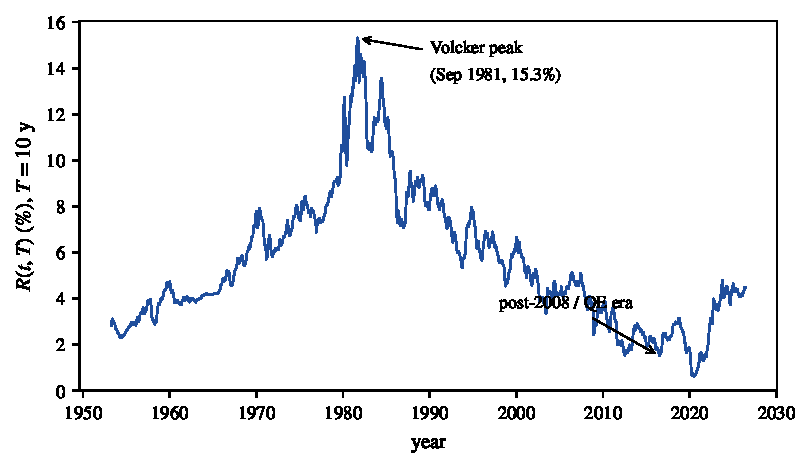
\includegraphics[width=0.9\textwidth]{images/treasury_10y.pdf}
\caption{US 10-Year Treasury constant-maturity yield, monthly averages, 1953--2026. Data: FRED, series GS10 (Federal Reserve Bank of St.\ Louis). Generated by \texttt{images/code\_for\_images/treasury\_10y.py}.}
\label{fig:treasury}
\end{figure}


\section{The yield to maturity and the yield curve}

If the growth rate of a bond is no longer constant, the exponent in $B(T)=B(t)\,e^{r(T-t)}$ must be replaced by an effective, maturity-dependent rate.
One writes
\begin{equation}
B(T) = B(t)\, e^{R(t,T)(T-t)},
\end{equation}
where $R(t,T)$ is the \emph{yield to maturity} (rendimento a scadenza): the constant rate that, applied over $[t,T]$, would reproduce the actual growth of the bond.
It depends on both the present time $t$ and the maturity $T$.
Using the normalization $B(T)=1$ and solving for $R$,
\begin{equation}
B(t) = e^{-R(t,T)(T-t)}
\;\Longrightarrow\;
\ln B(t) = -R(t,T)(T-t)
\;\Longrightarrow\;
R(t,T) = -\frac{1}{T-t}\,\ln B(t).
\end{equation}
So the market prices of bonds determine $R(t,T)$, and plotting it against the maturity $T$ at fixed $t$ produces the \emph{yield curve} (curva dei rendimenti) --- the single most watched graph in fixed income, to which we return in the final section.

From the yield to maturity one recovers the instantaneous rate as the short-maturity limit,
\begin{equation}\label{eq:spot-rate}
r(t) := \lim_{(t-T)\to 0} R(t,T) = \lim_{(t-T)\to 0}\Bigl(-\frac{1}{T-t}\ln B(t)\Bigr),
\end{equation}
which is formally indeterminate --- $B(T)=1$ makes the numerator vanish together with the denominator --- but converges, exactly as a derivative does.
The \emph{spot rate} $r(t)$ is the object our stochastic models will describe.


\section{The Vasi\v{c}ek model for bond pricing}\label{sec:vasicek-model}

The bond pricing model of Vasi\v{c}ek\cite{Vasicek1977} stands to bonds as Black--Scholes stands to options, and we will construct it along the same lines: hypotheses, hedged portfolio, no-arbitrage, PDE.

\paragraph*{Hypotheses.}

\begin{enumerate}[label=(\roman*)]
    \item There is market risk, but no credit risk.
    \item The short rate is assumed to be a Markov It\^o diffusion.
    \item The no-arbitrage principle holds.
    \item The interest rate follows the SDE
    \begin{equation}\label{eq:rate-sde}
    dr(t) = f(r,t)\,dt + S(r,t)\, dW_t,
    \end{equation}
    with drift and diffusion functions $f$ and $S$ to be specified later.
\end{enumerate}
The parallel with the stock case, $dS(t) = \mu S\,dt + \sigma S\,dW_t$, is deliberate, but the analogy must be handled with care: there, the underlying $S$ was a \emph{tradable} asset; here, one cannot buy ``one unit of interest rate''.
The chain of dependence is $r \to dr \to B(r,t;T)$, in parallel with $S \to dS \to O(S,t)$.

Let us compute how a bond price responds to the rate.
Given $B = B(r,t; T)$, It\^o's formula applied along~\eqref{eq:rate-sde} gives
\begin{equation}
dB = \biggl(\frac{\partial B}{\partial t} + f(r,t)\frac{\partial B}{\partial r} + \frac{1}{2}S^2(r,t)\frac{\partial^2 B}{\partial r^2}\biggr)dt + S(r,t)\frac{\partial B}{\partial r}\, dW_t.
\end{equation}
It is convenient to give names to the relative drift and volatility of the bond.\footnote{The notation follows the notes: $\mu$ and $\sigma$ here refer to the bond's return and volatility, not the stock's.}
We define
\begin{align}
\mu(t,T) &= \frac{1}{B(r,t;T)}\biggl(\frac{\partial B}{\partial t} + f(r,t)\frac{\partial B}{\partial r} + \frac{1}{2}S^2(r,t)\frac{\partial^2 B}{\partial r^2}\biggr), \\[4pt]
\sigma(t,T) &= -\frac{1}{B(r,t;T)}\, S(r,t)\,\frac{\partial B}{\partial r} > 0,
\end{align}
so that $\mu(t,T)$ is the instantaneous return of the bond and $\sigma(t,T)$ its volatility.
The minus sign in the definition of $\sigma$ is a sign convention chosen to make $\sigma$ positive, and it encodes a genuine piece of economics: the rate and the bond price are \emph{anticorrelated}.
If $dr > 0$, i.e.\ $r(t+dt) > r(t)$, then $B(r+dr) < B(r)$, so $dB < 0$.
A concrete example: let $T = 1$ year and suppose the BCE raises the annual rate from 2\% to 4\%.
Newly issued bonds now yield 4\%; the old ones, still promising 2\%, are suddenly less attractive, and their market price drops until their effective yield matches.

\subsection{The hedging portfolio}

We now look for the analogue of the delta-hedged portfolio.
There is an immediate obstruction: in Black--Scholes we hedged the option \emph{with the underlying stock}, but here the underlying is $r$, which cannot be held.
The resolution is to hedge \emph{one bond with another}: bonds of different maturities respond to the same $r$, so a suitable combination can be made riskless.

Let $B_i=B(r,t;T_i)$, $\mu_i=\mu(t,T_i)$ and $\sigma_i=\sigma(t,T_i)$.
Choose holdings $h_1,h_2$ and position values $V_i=h_iB_i$ in a self-financing portfolio of value $\Pi=V_2-V_1$.
Then
\[
 d\Pi=h_2\,dB_2-h_1\,dB_1
 =(V_2\mu_2-V_1\mu_1)\,dt-(V_2\sigma_2-V_1\sigma_1)\,dW_t.
\]
The holdings are adjusted so that $V_2\sigma_2=V_1\sigma_1$.
For $\sigma_1\ne\sigma_2$, the value and hedge conditions give
\[
 V_1=\frac{\Pi\sigma_2}{\sigma_1-\sigma_2},\qquad
 V_2=\frac{\Pi\sigma_1}{\sigma_1-\sigma_2}.
\]
Consequently the riskless portfolio satisfies
\[
 d\Pi=\Pi\frac{\mu_2\sigma_1-\mu_1\sigma_2}{\sigma_1-\sigma_2}\,dt=r\Pi\,dt,
\]
and hence
\[
 \sigma_1(\mu_2-r)=\sigma_2(\mu_1-r).
\]
The adjustable quantities are the holdings, not the quoted bond prices.
This is the same self-financing condition used in Chapter~5.

Rearranging so that each maturity keeps to its own side,
\begin{equation}\label{eq:vasicek-identity}
\frac{\mu(t,T_1) - r}{\sigma(t,T_1)} = \frac{\mu(t,T_2) - r}{\sigma(t,T_2)},
\end{equation}
valid $\forall\, t \le \min(T_1, T_2)$ and, crucially, $\forall\, T_1, T_2$.
This is the \textbf{Vasi\v{c}ek identity}, a dynamic identity of the model: the excess return per unit of volatility, $\frac{\mu - r}{\sigma}$, is the \emph{same for all bonds}, whatever their maturity --- a kind of separation of variables, with the maturity dropping out of the ratio.

\paragraph*{The market price of risk.}

Since the ratio in~\eqref{eq:vasicek-identity} does not depend on the maturity, it defines a function of $r$ and $t$ alone.
We give it a name:
\begin{equation}\label{eq:market-price-risk}
q(r,t) := \frac{\mu(r,t;T) - r}{\sigma(r,t;T)},
\end{equation}
the \emph{market price of risk}.
It measures the compensation --- excess return per unit of volatility --- that the market demands for bearing interest-rate risk, i.e.\ the aggregate risk aversion of bond investors.
In Black--Scholes no such object appeared, because hedging with the tradable underlying eliminated the risk premium entirely; here, where $r$ is not tradable, a residue of the market's attitude toward risk survives in the pricing equation.

To obtain that equation, write $q\,\sigma = \mu - r$ and substitute the definitions of $\mu$ and $\sigma$; the terms reassemble into
\begin{equation}\label{eq:term-structure}
\boxed{\frac{\partial B}{\partial t} + \bigl(f + S\,q\bigr)\,\frac{\partial B}{\partial r} + \frac{1}{2}S^2\,\frac{\partial^2 B}{\partial r^2} = r\, B}
\end{equation}
with boundary condition $B(r, t=T; T) = 1$.
This is the \textbf{term structure equation}, the exact analogue of the Black--Scholes equation $\partial_t O(S,t) + \ldots = rO$ for bonds.

Several remarks are in order before we solve it.
First, note the structural difference from Black--Scholes: there the discounting rate $r$ on the right-hand side was a fixed constant, while here the $r$ multiplying $B$ is the fluctuating state variable itself --- the same symbol, two very different roles.
Second, the equation is not yet specified: the functional forms of $f$ and $S$ must be modelled, and GBM will \emph{not} do --- an interest rate does not grow exponentially (if it did, no state could ever afford to issue bonds).
Third, taking $q$ constant is an additional modelling assumption, not a consequence of the ratio defining it.
With the bond convention $dB/B=\mu\,dt-\sigma\,dW$, the Girsanov kernel of Section~\ref{sec:rn-girsanov} is $\varphi=q$.
Thus $dW=q\,dt+dW^Q$ and the short-rate drift under $Q$ is $f+Sq$.
Finally, the Feynman--Kac formula of Chapter~5 offers an alternative representation of the solution,
\begin{equation}
B(r,t;T) = E^Q\!\Bigl[\exp\Bigl\{-\int_t^T r(s)\,ds\Bigr\}\,\Bigm|\,r(t)=r\Bigr],
\end{equation}
a discounted expectation as before --- except that now $r(s)$ is stochastic, so the discount factor sits \emph{inside} the expectation, integrated along each trajectory.
One could evaluate this average directly, but we will follow the PDE route instead.


\section{The Vasi\v{c}ek solution}\label{sec:vasicek-solution}

\subsection{The Ornstein--Uhlenbeck model for the interest rate}

To make the term structure equation concrete we must choose the model
\begin{equation}\label{eq:vasicek-sde}
dr(t) = f(r,t)\, dt + S(r,t)\, dW_t,
\end{equation}
i.e.\ commit to functional forms for $f$ and $S$.
What do we require of a sensible rate model?
That for long times $r$ neither explodes nor collapses, but hovers around a stable level with small fluctuations --- exactly the behaviour of the mean-reverting process we solved in Chapter~4.
Vasi\v{c}ek's choice is indeed the Ornstein--Uhlenbeck process\cite{UhlenbeckOrnstein1930}, shifted to revert to a nonzero level: the (essentially unique, by Doob's theorem) Markov, Gaussian, stationary process.
Its It\^o SDE is
\begin{equation}\label{eq:ou-rate}
dr(t) = \alpha\bigl[\theta - r(t)\bigr]dt + \sigma\, dW_t,
\end{equation}
with $\alpha, \theta, \sigma > 0$ and $[\alpha] = [t]^{-1} = \tau^{-1}$.
Here $\theta$ is the \emph{long-run mean} toward which the rate is pulled, and we note already that $\theta$ is \emph{not} simply the historical mean of the observed time series.\footnote{Under the historical measure, $\theta$ is the long-run mean and can be estimated from sufficiently long rate data.
The pricing parameter is the risk-adjusted mean $\theta^*$ defined below. See Section~\ref{sec:vasicek-calibration}.}

Although the solution parallels Chapter~4, we spell it out, both because the nonzero mean changes the formulas and because the notes' derivation is compact.
% CLAUDE NOTE: The notes' intermediate steps for the variable change are somewhat
% compressed (they write f(r,t) = r e^{αt} and a chain of substitutions x:=E, f(x)=x²=r).
% We present the standard derivation of the OU solution via Doob's transform.
Apply It\^o's lemma to the function $g(r,t) = r\, e^{\alpha t}$, for which $\partial_r g = e^{\alpha t}$ and $\partial_t g = \alpha r\, e^{\alpha t}$:
\begin{equation}
dg(r,t) = \bigl[\alpha r\, e^{\alpha t} + \alpha(\theta - r)\, e^{\alpha t}\bigr]dt + \sigma\, e^{\alpha t}\, dW_t = \alpha\theta\, e^{\alpha t}\, dt + \sigma\, e^{\alpha t}\, dW_t;
\end{equation}
the mean-reverting drift has been absorbed, by the integrating factor, and only an inhomogeneous source survives.
Integrating from $t$ to $T$ (where $T$ is a sufficiently long time),
\begin{equation}
r(T)\, e^{\alpha T} - r(t)\, e^{\alpha t} = \alpha\theta\int_t^T e^{\alpha s}\, ds + \sigma\int_t^T e^{\alpha s}\, dW_s,
\end{equation}
and solving for $r(T)$,
\begin{equation}\label{eq:ou-solution}
r(T) = \theta\bigl(1 - e^{-\alpha(T-t)}\bigr) + r(t)\, e^{-\alpha(T-t)} + \sigma\, e^{-\alpha T}\int_t^T e^{\alpha s}\, dW_s.
\end{equation}
The terms have a direct interpretation: the initial rate decays away exponentially, the long-run mean $\theta$ fades in to replace it, and the noise accumulates with exponentially fading memory.

The moments follow at sight.
The It\^o integral averages to zero, so
\begin{equation}
\mathbb{E}[r(T)\mid r(t)] = \theta\bigl(1 - e^{-\alpha(T-t)}\bigr) + r(t)\, e^{-\alpha(T-t)} \;\xrightarrow{T-t \gg \tau}\; \theta,
\end{equation}
and the mean converges to $\theta$ for long times --- the long-run economic average.
By the It\^o isometry,
\begin{equation}
\mathrm{Var}[r(T)\mid r(t)] = \sigma^2\, e^{-2\alpha T}\int_t^T e^{2\alpha s}\, ds = \frac{\sigma^2}{2\alpha}\bigl(1 - e^{-2\alpha(T-t)}\bigr) \;\xrightarrow{T-t \gg \tau}\; \frac{\sigma^2}{2\alpha},
\end{equation}
so the fluctuations saturate rather than growing without bound.
The process being Gaussian at all times,
\begin{equation}
\begin{gathered}
r(T)\mid r(t)\sim\mathcal N\!\left(\theta+(r(t)-\theta)e^{-\alpha(T-t)},\,
\frac{\sigma^2}{2\alpha}(1-e^{-2\alpha(T-t)})\right),\\
r(T)\mid r(t)\ \xrightarrow[T-t\to\infty]{\mathrm{law}}\
\mathcal N\!\left(\theta,\frac{\sigma^2}{2\alpha}\right).
\end{gathered},
\end{equation}
% Codex NOTE (2026-09-06): The previous theta/sigma expression is dimensionally inconsistent; expansion of the conditional OU mean gives alpha(theta-r).
while for short times the mean expands as $\mathbb{E}[r(T)\mid r(t)=r] = r + \alpha(\theta-r)(T-t) + O((T-t)^2)$

The qualitative behaviour has a name that finance uses constantly: \emph{mean reversion}.
Reading the SDE over an infinitesimal step,
\begin{equation}
dr(t) = r(t+dt) - r(t) = \alpha[\theta - r(t)]\,dt + \sigma\,dW_t,
\end{equation}
the deterministic part acts like a restoring force: whenever the rate sits above $\theta$ it is pushed down, whenever below, up, and the trajectory keeps oscillating around the mean (Figure~\ref{fig:mean-reversion}).
Taking the ensemble average of the increment,
\begin{equation}
\mathbb{E}\bigl[r(t+dt) - r(t)\bigr] = \alpha\bigl[\theta - \mathbb{E}[r(t)]\bigr]\, dt,
\end{equation}
which identifies $\alpha$ as the \emph{speed of mean reversion}: it quantifies how fast the rate returns to $\theta$ after a fluctuation.
In simulations one averages finitely many trajectories; this estimates the ensemble relaxation with sampling error.

\begin{figure}[h!]
\centering
\begin{tikzpicture}
    \draw[->] (0,0) -- (6,0) node[right] {$t$};
    \draw[->] (0,0) -- (0,3) node[above] {$r$};
    \draw[dashed, gray] (0,1.5) -- (6,1.5) node[right, font=\footnotesize] {$\theta$};
    \draw[thick, blue, domain=0:5.8, samples=200]
        plot (\x, {1.5 + 0.8*exp(-0.5*\x)*cos(200*\x) + 0.3*sin(150*\x)*exp(-0.2*\x)});
\end{tikzpicture}
\caption{Mean reversion in the Vasi\v{c}ek model: the rate $r(t)$ oscillates around the long-run mean $\theta$, pulled back by the restoring drift at speed $\alpha$.}
\label{fig:mean-reversion}
\end{figure}

The model has one well-known blemish.
Being Gaussian with unbounded support, the rate can fluctuate to \emph{negative} values, especially at long times if $\theta$ is small.
In principle this should not happen; in practice, remarkably, bonds with negative yields \emph{have} existed --- marginally around 2008, then systematically in Europe and Japan --- so the blemish is partly a feature.\footnote{Negative yields can be read as an insurance premium: investors accept a small guaranteed loss --- a contained loss, compared with other assets --- in exchange for safety; central-bank policy did the rest.
For example, the Swiss National Bank set its sight-deposit rate at $-0.75\%$ in January 2015; longer-dated Swiss government bonds also traded at negative yields. See the SNB's October 2016 policy discussion\cite{SNB2016}.}
% CLAUDE NOTE: The notes mention "2008" for negative rates; the phenomenon was
% systematic during 2014-2021 in the eurozone, Switzerland, and Japan (footnote expanded
% at the author's request, 2026-07-02).

An alternative is the nonnegative CIR model\cite{CIR1985}.
The construction in the handwritten notes starts from a Gaussian OU variable $x$, whose square is $r=x^2$:
\begin{equation}\label{eq:cir-sde}
 dx=-\gamma x\,dt+\delta\,dW_t.
\end{equation}
The variable $x$ is signed; it cannot be identified with the nonnegative square root $\sqrt r$.
It\^o's formula gives
\[
 dr=(\delta^2-2\gamma r)\,dt+2\delta x\,dW_t
 =\alpha(\theta-r)\,dt+\sigma\sqrt r\,d\widetilde W_t,
\]
where $\alpha=2\gamma$, $\theta=\delta^2/(2\gamma)$, $\sigma=2\delta$, and $d\widetilde W_t=\operatorname{sgn}(x_t)dW_t$ (take the sign at zero to be $1$).
The process $\widetilde W$ is Brownian, since its quadratic variation is $t$.
This construction gives a special CIR parameter choice, not the general model.\footnote{The general CIR diffusion permits independent positive $\alpha,\theta,\sigma$.
Starting from $r>0$, the Feller condition $2\alpha\theta\ge\sigma^2$ ensures that zero is not reached; otherwise zero can be reached, although the process remains nonnegative.
The squared-OU construction above does not satisfy this condition.
The finite-time transition law is a scaled noncentral chi-squared distribution, and the stationary law is Gamma, with shape $2\alpha\theta/\sigma^2$ and rate $2\alpha/\sigma^2$\cite{CIR1985,Bjork2020}.}

\begin{figure}[h!]
\centering
\begin{tikzpicture}
    \draw[->] (0,0) -- (4,0) node[right] {$r(t)$};
    \draw[->] (0,0) -- (0,2.5) node[above] {$P_{\mathrm{stat}}(r)$};
    \draw[thick, blue, domain=0.05:3.8, samples=80]
        plot (\x, {\x*exp(-\x)});
    \node[font=\footnotesize] at (2.5, 1.8) {Gamma density};
\end{tikzpicture}
\caption{An illustrative stationary CIR Gamma density, with shape $2$ and rate $1$ in scaled rate units.
These parameters describe a general CIR model, not the special squared-OU construction above.}
\label{fig:cir-chi2}
\end{figure}

Yet another route to positivity is the \emph{exponential Vasi\v{c}ek} model, obtained by modelling the \emph{logarithm} of the rate as an OU process:
\begin{equation}
Y(t) = \ln r(t) \quad\Longrightarrow\quad r(t) = \exp\{Y(t)\} > 0,
\end{equation}
so that $r$ is log-normal --- approximately what one sees in the data.

\subsection{Solution of the term structure equation}\label{sec:vasicek-term-structure}

We now return to the term structure equation~\eqref{eq:term-structure} and solve it with the OU specification.
Assuming constant $q$ and substituting $f = \alpha(\theta-r)$ and $S=\sigma$, the drift correction combines with the market price of risk into
\begin{equation}
f + S\,q = \alpha(\theta^* - r),
\qquad
\theta^* = \theta + \frac{\sigma\,q}{\alpha},
\end{equation}
% CLAUDE NOTE: θ* is the risk-adjusted long-run mean: θ shifted by the market price of risk.
so the whole effect of risk aversion is to shift the long-run mean from $\theta$ to the \emph{risk-adjusted} value $\theta^*$ --- an economical piece of bookkeeping.
The problem is then
\begin{equation}
\frac{\partial B}{\partial t} + \alpha(\theta^*-r)\,\frac{\partial B}{\partial r} + \frac{1}{2}\sigma^2\,\frac{\partial^2 B}{\partial r^2} = r\, B, \qquad B(T) = 1.
\end{equation}

The equation is linear in $r$ in its coefficients, which suggests an exponential-affine \emph{ansatz}:
\begin{equation}
P(r,t;T) = A(t,T)\, e^{-r\, B_0(t,T)},
\end{equation}
with terminal conditions $A(T,T) = 1$ and $B_0(T,T) = 0$ (so that $P(r,T;T)=1$ as required).
% CLAUDE NOTE: The notes use P for the trial solution and B₀ for the exponent coefficient
% to avoid confusion with the bond price B. We follow this convention.
The derivatives of the ansatz are
\begin{equation}
\partial_t P = \dot{A}\, e^{-rB_0} - r\dot{B}_0\, A\, e^{-rB_0},
\qquad
\partial_r P = -A\,B_0\,e^{-rB_0}, \qquad \partial^2_r P = A\,B_0^2\,e^{-rB_0},
\end{equation}
and substituting into the PDE and dividing through by $A\, e^{-rB_0}$,
\begin{equation}
\frac{\dot{A}}{A} - r\dot{B}_0 - \alpha(\theta^*-r)\,B_0 + \frac{1}{2}\sigma^2\,B_0^2 = r.
\end{equation}
Now comes the decisive observation: this must hold \emph{for every value of $r$}, and $r$ appears only linearly.
The coefficient of $r$ and the $r$-independent part must therefore vanish \emph{separately} --- the PDE splits into two ordinary differential equations.

Collecting the terms linear in $r$ (including the right-hand side),
\begin{equation*}
-\dot{B}_0 + \alpha B_0 - 1 = 0 \quad\Longrightarrow\quad \dot{B}_0 = \alpha B_0 - 1,
\qquad\text{(a)}
\end{equation*}
and collecting the constant terms,
\begin{equation*}
\frac{\dot{A}}{A} - \alpha\theta^*\,B_0 + \frac{1}{2}\sigma^2\,B_0^2 = 0.
\qquad\text{(b)}
\end{equation*}

Equation (a) is a linear first-order ODE.
Its general solution is $B_0(t,T) = Ce^{\alpha t} + \frac{1}{\alpha}$, and imposing $B_0(T,T)=0$ fixes $C = -\frac{1}{\alpha}\,e^{-\alpha T}$, whence
\begin{equation}\label{eq:vasicek-B}
B_0(t,T) = \frac{1}{\alpha}\bigl(1 - e^{-\alpha(T-t)}\bigr).
\end{equation}
Note the two limits: $B_0\approx T-t$ for short maturities (the bond behaves like $e^{-r(T-t)}$, as it must), while $B_0\to1/\alpha$ for long maturities --- mean reversion caps the sensitivity of long bonds to the current rate.

With $B_0$ known, equation (b) determines $A$ by separation of variables:
\begin{equation}
\frac{dA}{A} = \Bigl[\alpha\theta^*\,B_0 - \frac{1}{2}\sigma^2\,B_0^2\Bigr]dt,
\end{equation}
with $A(T,T) = 1$, i.e.\ $\ln A(T,T) = 0$.
Integrating from $t$ to $T$,
\begin{equation}
\ln A(t,T) = \int_t^T \bigl[-\alpha\theta^* B_0(s,T) + \tfrac12\sigma^2 B_0^2(s,T)\bigr]ds,
\end{equation}
and carrying out the (elementary if tedious) integrals yields
\begin{equation}\label{eq:vasicek-A}
\ln A(t,T) = \Bigl(\theta^* - \frac{\sigma^2}{2\alpha^2}\Bigr)\bigl[B_0(t,T) - (T-t)\bigr] - \frac{\sigma^2}{4\alpha}\,B_0^2(t,T),
\end{equation}
% CLAUDE NOTE: This is equivalent to the formula
% ln A = (θ* - σ²/2α²)[(1-e^{-α(T-t)})/α - (T-t)] - σ²/(4α) · [(1-e^{-α(T-t)})/α]²
which passes the sanity check $\ln A(T,T)=0$, since both $B_0(T,T)$ and $T-T$ vanish.

Assembling the pieces, the Vasi\v{c}ek bond price is
\begin{equation}
P(r,t;T) = A_{\text{Vas}}(t,T)\, e^{-r\,B_0(t,T)} =: P_{\text{Vas}}(r,t;T;\, \alpha, \theta^*, \sigma),
\end{equation}
an explicit closed formula --- the bond-market counterpart of the Black--Scholes formula.


\section{Calibration}\label{sec:vasicek-calibration}

A pricing formula is only useful once its parameters are pinned to the market, and the Vasi\v{c}ek model has three: $\alpha$, $\sigma$, and $\theta^*$.
The yield to maturity gives us the handle.
On the empirical side,
\begin{equation}
R(t,T) = -\frac{1}{T-t}\,\ln P(r,t;T) \quad\longrightarrow\quad \text{measured from quoted bond prices},
\end{equation}
while on the theoretical side the model predicts
\begin{equation}
R_v(r,t;T;\,\alpha,\theta^*,\sigma) = -\frac{1}{T-t}\,\ln P_v(r,t;T;\,\alpha,\theta^*,\sigma).
\end{equation}
The pricing mean $\theta^*$ must be inferred from market prices as well as historical dynamics.\footnote{The phrase ``tirato fuori dal mercato'' is a paraphrase in the handwritten lecture notes, not a verified quotation from Bj\"ork.
For the distinction between historical dynamics and pricing dynamics, see Bj\"ork\cite{Bjork2020}, the chapters on short-rate models.}


The calibration proceeds in two steps, each using the data best suited to it.
First, one fits $\alpha$ and $\sigma$ --- the dynamical parameters --- from the historical time series of the spot rate $r(t)$, by a best fit of the observed relaxation and fluctuations.
Second, one fits $\theta^*$ --- the risk-adjusted level, invisible in the history because it contains the market price of risk --- from today's \emph{yield curve}: at the observed maturities ($1, 2, 3, 4, 5, 10, 20$ years, \ldots) one imposes
\begin{equation}
R_{\text{emp}}(t,T) - R_{\text{the}}(r,t;T;\,\alpha,\sigma,\theta^*) = 0
\end{equation}
and fits $\theta^*$, generally by minimizing the discrepancies over maturities; one parameter need not match every quoted yield exactly.
Figure~\ref{fig:yield-curve} illustrates an upward-sloping model curve with synthetic observations; it is not an empirical calibration.

\begin{figure}[h!]
\centering
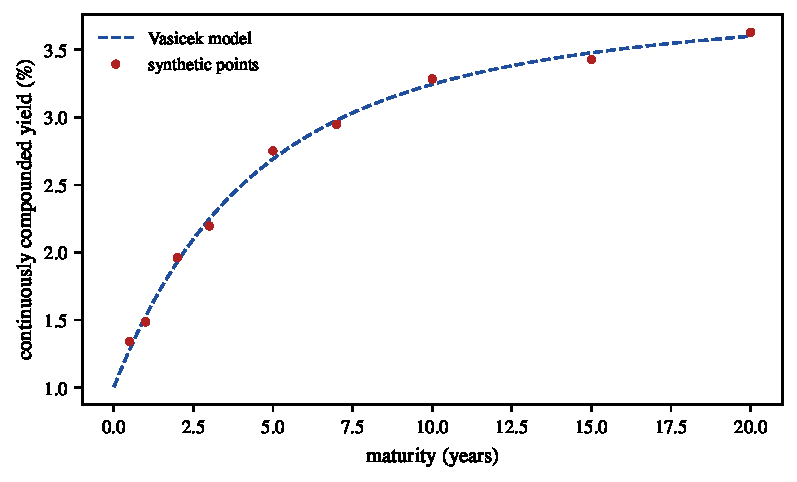
\includegraphics[width=0.72\textwidth]{images/vasicek_yield_review.pdf}
\caption{Illustrative Vasi\v{c}ek yield curve ($r=1\%$, $\alpha=0.4$, $\theta^*=4\%$, $\sigma=1\%$ in annual units), with synthetic perturbed points.
No market data were fitted.}
\label{fig:yield-curve}
\end{figure}

With all parameters fixed, the model prices not only the bonds themselves but the derivatives written on them: in the market one actively trades \emph{bond options}, whose valuation depends on exactly the parameters just calibrated.
The interplay between an analytically solvable model and a market calibration is the same we met for Black--Scholes --- and, as there, the model's Gaussian simplicity is both its strength and its limitation.
The next chapter confronts those limitations head-on.


\chapter{Advanced Financial Models}

The Black--Scholes framework rests on two statistical pillars: log-returns are Gaussian, and volatility is constant.
Chapter~5 already hinted, through the volatility smile, that the market itself does not believe either.
In this chapter we confront the model with the data and repair it in two directions.
First, we introduce the \emph{stable distributions} of L\'evy, whose fat tails describe the empirical statistics of returns far better than the Gaussian; second, we promote the volatility to a stochastic process of its own, obtaining the \emph{stochastic volatility} models --- Stein--Stein, Heston, and their relatives --- that are the workhorses of modern quantitative finance.
The chapter closes by redoing Black--Scholes in the Heston world, where a new and instructive obstacle appears: volatility cannot be hedged with the stock alone.
% CLAUDE NOTE (unreviewed PDF): These notes are unreviewed but "mostly good."
% Original reasoning is preserved; expansions and corrections are noted in comments.

Before any statistics, Figure~\ref{fig:sp500-vs-gbm} explains both why the GBM conquered finance and why this chapter is necessary.
The upper panel shows ten years of the real S\&P\,500; the lower panel shows a geometric Brownian motion simulated with the \emph{same} drift and the \emph{same} volatility, estimated from those very data.
At a glance the two are remarkably alike --- same trend, same jitter, same look at every scale --- which is precisely the mimicry that made the GBM the default model of Chapter~5.
Look longer, though, and the real series gives itself away: the cliff of February--March 2020, when the index lost a third of its value in four weeks with single days beyond $-12\%$, has no counterpart in the simulated panel --- and never will, because in a Gaussian world a $12\sigma$ day is not rare but essentially impossible.
Everything that follows in this chapter is, in one way or another, the statistics of that difference.

% Real-data figure; generated by images/code_for_images/sp500_returns.py from FRED series SP500.
\begin{figure}[h!]
\centering
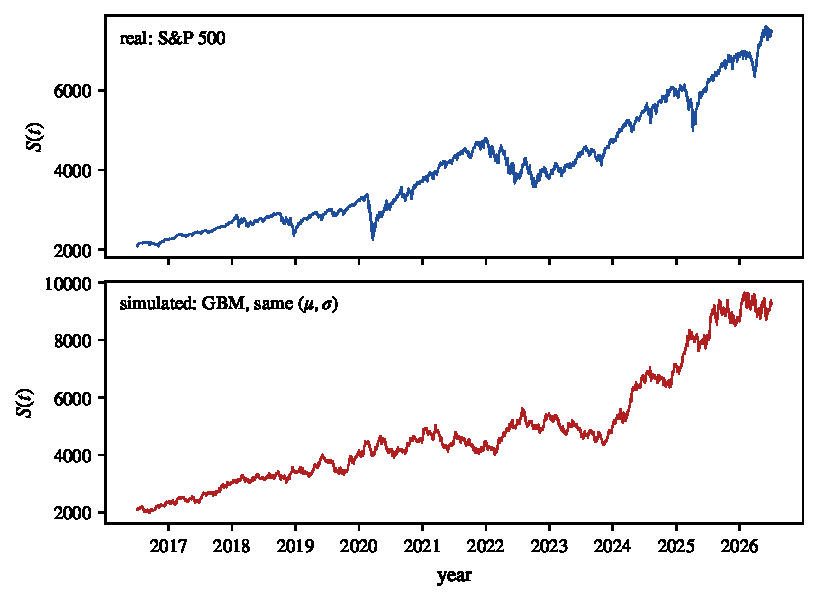
\includegraphics[width=0.88\textwidth]{images/sp500_vs_gbm.pdf}
\caption{Top: the S\&P\,500, daily closes 2016--2026 (FRED series SP500). Bottom: a geometric Brownian motion simulated with the same starting value and the same daily drift and volatility estimated from the data. The two are nearly indistinguishable by eye --- except for the 2020 crash in the real series, whose violence the Gaussian model cannot produce. Generated by \texttt{images/code\_for\_images/sp500\_returns.py}.}
\label{fig:sp500-vs-gbm}
\end{figure}


\section{Empirical properties of log-returns}

Let us first recall what the GBM predicts, so that we know exactly what to test.
For $dS = \mu S\,dt + \sigma S\,dW_t$, the log-returns satisfy
\begin{equation}
\mathbb{E}\!\biggl[\ln\frac{S(t+\Delta t)}{S(t)}\biggr] = \mu^*\Delta t, \qquad \mu^* = \mu - \frac{\sigma^2}{2},
\qquad
\mathrm{Var}\!\biggl[\ln\frac{S(t+\Delta t)}{S(t)}\biggr] = \sigma^2\Delta t,
\end{equation}
and shifting the time window, $t\to t+\tau$, $t+\Delta t\to t+\Delta t+\tau$, changes nothing: the returns are stationary, consistent with $\delta t = t_j - t_i = (t_j + \Delta t) - t_j$.
For the price itself the model gives
\begin{equation}
\mathbb{E}[S(t)] = S_0\, e^{\mu t}, \qquad \mathrm{Var}[S(t)] = S_0^2\, e^{2\mu t}\bigl(e^{\sigma^2 t}-1\bigr),
\end{equation}
although in reality $\mu$ itself changes over the years --- a first warning sign.

The decisive test is the histogram.
Take a real time series, compute the log-returns, extract the empirical mean and standard deviation $\mu_e \leftrightarrow m$, $\sigma_e \leftrightarrow s$, and superimpose on the histogram the Gaussian that the model predicts,
\begin{equation}
\mathrm{PDF}\!\bigl\{\ln r_{\Delta t}(t)\bigr\} \approx \mathcal{N}(\mu_e, \sigma_e) = \frac{1}{\sqrt{2\pi\sigma_e^2}}\,\exp\!\biggl\{-\frac{(\ln r_{\Delta t}(t) - \mu_e)^2}{2\sigma_e^2}\biggr\}.
\end{equation}
The fit fails, and it fails in a characteristic way, shown on real data in Figure~\ref{fig:sp500-hist}: the empirical distribution is far more peaked at the centre and, above all, far heavier in the tails.
Extreme returns --- crashes and rallies --- occur orders of magnitude more often than any Gaussian allows.
The returns are \emph{not} normally distributed, and we need a family of distributions built to accommodate this.

% Figure after the course slides; generated by images/code_for_images/sp500_stylized.py
\begin{figure}[h!]
\centering
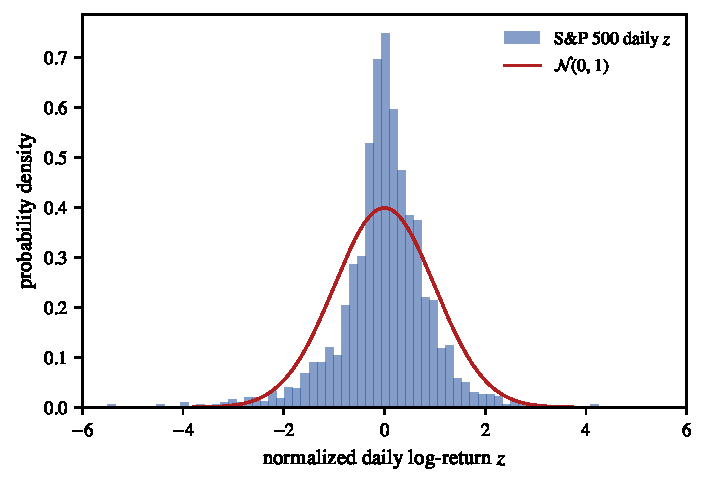
\includegraphics[width=0.72\textwidth]{images/sp500_hist.pdf}
\caption{The histogram test on real data: normalized daily log-returns of the S\&P\,500 (2016--2026, FRED series SP500) against the Gaussian with the same mean and variance. The empirical distribution has a sharper central body and far heavier tails --- returns beyond $\pm4\sigma$, essentially impossible for the Gaussian, are clearly populated. Generated by \texttt{images/code\_for\_images/sp500\_stylized.py}.}
\label{fig:sp500-hist}
\end{figure}


\section{Stable distributions}\label{sec:stable-distributions}

The appropriate family was identified by L\'evy, and imported into finance by Mandelbrot: the \emph{stable distributions}, whose theory is also known as the \emph{generalized Central Limit Theorem} (generalized CLT), with contributions by Gnedenko.
Why ``generalized''?
The ordinary CLT says that sums of i.i.d.\ variables with \emph{finite variance} converge to the Gaussian; the generalized version asks the bolder question --- what are \emph{all} the possible limits of such sums, finite variance or not? --- and the answer is precisely the stable family.

A stable distribution is characterized by four interlocking properties, which we examine in turn: stability under convolution, a closed-form characteristic function, power-law asymptotic behaviour, and the corresponding cumulative distribution function (CDF).

\subsection{Stability}

Let $X_1, X_2$ be i.i.d.\ random variables with PDF $P(x)$, so that $P_2(x_1, x_2) = P(x_1)P(x_2)$, and consider their sum $S_2 = X_1 + X_2$ (so that $X_2 = S_2 - X_1$).
The PDF of the sum is the convolution
\begin{equation}
P_2(S_2) = \int dx\, P(x)\, P(S_2 - x) = P * P.
\end{equation}
Convolutions are unwieldy; Fourier transforms turn them into products.
Defining the \emph{characteristic function} $\tilde\phi(k)=\mathcal{F}[P]$,
\begin{equation}
\mathcal{F}\bigl[P_2(S_2)\bigr] = \tilde\phi_2(k) = \int dx\, e^{ikx}\, P_2(S_2) = \mathcal{F}[P*P] = \mathcal{F}[P]\cdot\mathcal{F}[P] = \tilde\phi^2(k),
\end{equation}
and for $N$ i.i.d.\ variables $X_1,\ldots,X_N$ with $S_N = \sum_{i=1}^{N} X_i$,
\begin{equation}
\mathcal{F}[P_2(S_N)] = \tilde\phi^N(k),
\end{equation}
generically a leptokurtic (heavy-tailed relative to its width) distribution.
A distribution is called \emph{stable} when this operation does not change its shape: the sum has the same distribution as the summands, up to a rescaling.

The Gaussian is the prototype.
For $P_0(x) = \frac{1}{\sqrt{2\pi}\sigma}\, e^{-x^2/(2\sigma^2)}$, with scale parameter $\sigma$, the characteristic function is
\begin{equation}
\tilde\Phi(k) = \int dx\, e^{ikx}\, P_0(x) = \exp\!\Bigl\{-\frac{\sigma^2 k^2}{2}\Bigr\},
\end{equation}
so that
\begin{equation}
\tilde\phi_2(k) = \mathcal{F}[P*P] = e^{-\sigma^2 k^2} \quad\Longrightarrow\quad \mathcal{F}^{-1}[\tilde\phi_2(k)] = P_0(x, N=2):
\end{equation}
the sum of two Gaussians is again a Gaussian --- the Gaussian is stable.
How does the scale grow?
Rewriting the $N=2$ result,
\begin{equation}
P_0(x, N=2) = \frac{1}{\sqrt{2\pi(2\sigma^2)}}\, \exp\!\biggl\{-\frac{x^2}{2\cdot 2\sigma^2}\biggr\} = \frac{1}{\sqrt{2}}\,\frac{1}{\sigma_2}\, P_0\!\Bigl(\frac{x}{\sigma_2}\Bigr),
\end{equation}
and in general
\begin{equation}
P_N(x, N) = \frac{1}{a_N}\, P_0\!\Bigl(\frac{x}{a_N}\Bigr), \qquad a_N = \sqrt{N}\, \sigma = N^{1/\alpha}\sigma, \quad \alpha = 2,
\end{equation}
where the $a_N$ are rescaling factors.
The exponent $\alpha$ appearing in $a_N = N^{1/\alpha}$ is the \emph{characteristic exponent} (or \emph{L\'evy index}) of the distribution; for the Gaussian, $\alpha=2$, which is just the familiar $\sqrt{N}$ growth of a random walk.
As we now see, other values of $\alpha$ are possible --- and each governs a different, self-consistent statistical world.

\subsection{The Cauchy distribution}

The most instructive non-Gaussian member of the family is the \emph{Cauchy} distribution (the Lorentzian of spectroscopy), which realizes $\alpha=1$:
\begin{equation}
P_c(x) = \frac{\delta}{\pi}\,\frac{1}{\delta^2 + x^2}, \qquad \delta = \text{scale parameter}.
\end{equation}
Its characteristic function is the two-sided exponential
\begin{equation}
\tilde\phi(k) = \mathcal{F}[P_c(x)] = e^{-\delta|k|},
\end{equation}
and stability is verified at sight:
\begin{equation}
\tilde\phi_2(k) = e^{-2\delta|k|} \quad\Longrightarrow\quad P_c(x, N=2) = \frac{2\delta}{\pi}\,\frac{1}{4\delta^2+x^2} = \frac{1}{a_2}\,P_c\!\Bigl(\frac{x}{a_2}\Bigr),
\end{equation}
a Cauchy again, with rescaling $a_N = N^{1/\alpha}$, $\alpha=1$: the scale of the sum grows \emph{linearly} in $N$, much faster than the Gaussian $\sqrt{N}$.
Asymptotically $P_c(x) \sim 1/x^{1+\alpha} = 1/x^{2}$ for $|x|\to\infty$, and this slow power-law decay has a startling consequence: the Cauchy distribution has \emph{no finite mean and no finite variance}.
It is a pathological but deeply instructive object --- a perfectly legitimate, normalizable distribution for which the standard toolkit of means and variances simply does not apply.
The family of stable laws interpolates between these behaviours, guided by the index $\alpha$.

\subsection{General $\alpha$-stable distributions}

For a general symmetric $\alpha$-stable distribution the characteristic function is
\begin{equation}
\tilde\phi_\alpha(k) = \exp\!\bigl\{-\delta|k|^\alpha\bigr\}, \qquad \forall\, \alpha \text{ admissible and } \delta \text{ (scale)},
\end{equation}
a \emph{stretched exponential} in $k$ for $\alpha\in(0,2)$.
The two cases already met are recovered as $\delta = \frac{\sigma^2}{2}$, $\alpha=2$ (Gaussian) and $\delta > 0$, $\alpha=1$ (Cauchy).
The admissible range is $0 < \alpha \le 2$, and within it the moments deteriorate progressively: for $1 < \alpha < 2$ the variance does not exist; for $0 < \alpha \le 1$ even the mean is gone.
Such distributions have no characteristic scale --- they are \emph{scale-free}.
The density itself is recovered by inverse Fourier transform,
\begin{equation}
P_\alpha(x) = \frac{1}{2\pi}\int dk\, e^{-ikx}\, e^{-\delta|k|^\alpha}, \qquad \int dx\, P_\alpha(x) = 1,
\end{equation}
which has closed form only in special cases ($\alpha=2$, $\alpha=1$), but whose properties are known in general.

\subsection{Asymptotic behaviour and CDF}

The third property is the one that matters most for data analysis: for every $\alpha<2$, the tails of the density decay as a \emph{power law},
\begin{equation}
P_\alpha(x) \propto \frac{C_\alpha}{|x|^{1+\alpha}}, \qquad |x|\to\infty.
\end{equation}
In practice one works with the fourth property, the cumulative distribution,
\begin{equation}
P_<(x) = \int_{-\infty}^{x}\! P(x')\, dx', \qquad P_>(x) = \int_x^{+\infty}\! P(x')\, dx' = 1 - P_<(x),
\end{equation}
because integrating the histogram tames the statistical noise in the tail.
Writing $\alpha' = \alpha + 1$ for the density exponent (so that $0 < \alpha' \le 3$ delimits the L\'evy regime), the tail of the CDF follows by direct integration:
\begin{equation}
P_>^*(x) = \int_x^{+\infty}\!dx'\; P_\alpha(x') \;\xrightarrow{|x|\to\infty}\; C_\alpha\int_x^{\infty}\!dx'\; x'^{-\alpha'} = \frac{C_\alpha}{\alpha'-1}\,x^{-(\alpha'-1)} = \frac{C_\alpha}{\alpha}\,x^{-\alpha}.
\end{equation}
Taking logarithms of both sides,
\begin{equation}
\ln P_>^*(x) = \ln\frac{C_\alpha}{\alpha} - \alpha\ln x,
\end{equation}
so in a \emph{log-log plot} the tail is a straight line of slope $-\alpha$: this is the standard experimental signature, and the standard way of measuring $\alpha$ from data (Figure~\ref{fig:loglog-tail}).
The contrast with the Gaussian could not be sharper: $\ln P_0(x) \sim -x^2$ plunges quadratically, while $\ln P_\alpha(x) \sim -\alpha\ln x$ descends along a gentle straight line --- the fat tail.

\begin{figure}[h!]
\centering
\begin{tikzpicture}
    \draw[->] (0,0) -- (5,0) node[right] {$\ln x$};
    \draw[->] (0,0) -- (0,3.5) node[above] {$\ln P_>^*(x)$};
    \draw[thick, blue, domain=0.5:4.5, samples=50] plot (\x, {3.0 - 0.6*\x});
    \node[blue, font=\footnotesize] at (4, 1.5) {slope $= -\alpha$};
    \draw[thick, red, dashed, domain=0.5:3, samples=50] plot (\x, {3.0 - 0.3*\x*\x});
    \node[red, font=\footnotesize] at (2.5, 0.3) {Gaussian};
\end{tikzpicture}
\caption{Tail of the cumulative distribution in a log-log plot: a stable law gives a straight line of slope $-\alpha$, while the Gaussian bends down quadratically. The straight-line tail is the experimental fingerprint of fat tails.}
\label{fig:loglog-tail}
\end{figure}

\subsection{Empirical evidence}

How do real markets score on this test?
The first measurement is due to Mandelbrot, who studied the daily log-returns of cotton prices and found a beautiful power-law tail with $\alpha \approx 1.7$; Fama repeated the analysis on stock returns with similar results (empirical analyses of asset prices for which Fama would receive the 2013 Nobel Prize in Economics).
% CLAUDE NOTE: the Fama Nobel mention is from the course slides, added 2026-07-06.
% CLAUDE NOTE: the notes attribute the stock-returns study to "Gnedenko (Fama)"; the standard
% reference for daily stock returns is Fama's 1965 study, while Gnedenko's contribution is the
% generalized CLT theory itself.
But a value $\alpha = 1.7 < 2$ is not acceptable at face value: it implies \emph{infinite variance}, hence in particular an undefined volatility --- awkward, for the quantity on which all of Chapter~5 was built.

The modern reference measurement is that of Mantegna and Stanley \cite{MantegnaStanley1995}, who analysed the S\&P\,500 at $\Delta t = 1$ minute over 1984--1989, using the standardized variable
\begin{equation}
z = \frac{\frac{\Delta S_{\text{SP}}(t)}{S(t)} - \mu}{\sigma},
\end{equation}
and found, once again, a stable-law behaviour with $\alpha \approx 1.4$.

The test is easy to repeat on modern data, and Figure~\ref{fig:sp500-ccdf} does so on ten years of daily S\&P\,500 closes.
The result is textbook material in the most literal sense: the empirical CCDF of the normalized returns tracks the Gaussian up to about two standard deviations and then departs from it spectacularly, following a straight power-law line of slope $\approx-3$ across the tail --- daily moves of $5\sigma$, which the Gaussian declares essentially impossible ($P_>\sim10^{-7}$), occur at the rate of a few per decade.
A CCDF slope of $-3$ corresponds to a density decaying as $|z|^{-4}$: this is precisely the \emph{inverse quartic law} that we are about to meet in the next subsection, and it lies \emph{outside} the L\'evy range $\alpha<2$ --- a first hint that the pure stable law cannot be the whole story.

% Real-data figure; generated by images/code_for_images/sp500_returns.py from FRED series SP500.
\begin{figure}[h!]
\centering
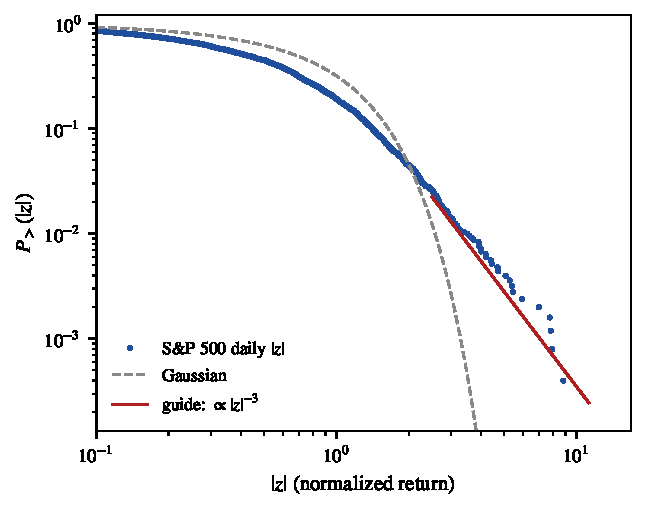
\includegraphics[width=0.62\textwidth]{images/sp500_ccdf.pdf}
\caption{Complementary CDF of the absolute normalized daily log-returns $|z|$ of the S\&P\,500 (2016--2026, FRED series SP500), in log-log scale, against the Gaussian prediction (dashed) and the inverse-cubic guide line $\propto|z|^{-3}$ (red). The fat tail --- the straight-line regime --- is the empirical refutation of the GBM hypothesis. Generated by \texttt{images/code\_for\_images/sp500\_returns.py}.}
\label{fig:sp500-ccdf}
\end{figure}
Two observations enrich the picture.
First, the S\&P\,500 aggregates $500$ assets, and its distribution is non-Gaussian because the components are \emph{not independent} --- when they fall, they fall together, so the standard CLT does not apply to the aggregation; disentangling such cross-correlations requires \emph{random matrix theory}.
Second, the scaling is impressive: the same law, with the same $\alpha$, holds across different time horizons $\Delta t$, with the PDF collapsing as $\mathrm{PDF}\{r(\Delta t)\} \sim \Gamma^*(\Delta t)$ and the CDF as $r^*(\Delta t)$ --- the self-similarity of stable laws at work in real data.

\subsection{Truncated stable distributions}

The resolution of the infinite-variance puzzle is that the true tail is \emph{not} a pure stable law all the way to infinity.
The far tail is better modelled by a power law \emph{truncated by an exponential},
\begin{equation}
P_{\alpha,\lambda}(x) \sim |x|^{-(1+\alpha)}\, e^{-\lambda|x|},
\end{equation}
% CLAUDE NOTE (unreviewed): the notes' exponent reads "(α−1)" with a positive sign, which
% would not be normalizable; the truncated Lévy distribution keeps the tail exponent −(1+α)
% of the pure stable law, multiplied by the exponential cutoff.
which preserves the stable behaviour over the observable range while restoring a finite variance.
An equally popular parametrization is the \emph{Student-$t$} distribution,
\begin{equation}
P_S(t) = C_S\biggl(1 + \frac{x^2}{v\hat\sigma^2}\biggr)^{-\frac{v+1}{2}},
\end{equation}
where $\hat\sigma$ is a scale parameter and $v$ a shape parameter (the number of degrees of freedom).
For $v=3$ the asymptotic tail decays as $x^{-4}$ --- the \emph{inverse quartic law} --- which is compatible with a large body of empirical observations.\footnote{The Student-$t$ arises naturally as a mixture of Gaussians whose variance is itself random ($\chi^2$-distributed) --- a first hint that random volatility and fat tails are two faces of the same phenomenon. This is the parametric approach to fitting the PDF of returns.}


\section{Volatility}\label{sec:adv-volatility}

The second pillar to re-examine is the volatility.
In reality $\sigma$ is not constant --- and worse, it is a \emph{hidden} quantity: no market quotes it directly, and extracting it is a delicate statistical task.
Throughout this section the basic observable is the log-return
\begin{equation}
dX_t = \ln\frac{S(t+\Delta t)}{S(t)} - S(t).
\end{equation}
% CLAUDE NOTE: The notes define dX as the log-return; the subtraction of S(t) is likely
% shorthand for the centered return (subtracting the mean μ*Δt).

Three estimators of volatility are in common use, in increasing order of temporal resolution.

The first is the \emph{historical volatility}, extracted from the sample variance of the time series, exactly as described in Chapter~5 (Section~\ref{sec:volatility}).

The second is the \emph{high-frequency volatility}, built from the mean absolute return rather than the squared one,
\begin{equation}
\sigma_{\text{hf}} = \frac{1}{N-1}\sum_{i=1}^{N}|dX_i|,
\end{equation}
with $\alpha$ the exponent of the associated $P(x)$.
To relate it to $\sigma$, assume for a moment Gaussian returns, $P(x)=\mathcal{N}(0,\sigma^2)$; then
\begin{equation}\begin{split}
\sigma_{\text{hf}} = \mathbb{E}[|x|] &= \int dx\,|x|\,P(x) = 2\int_0^{\infty}\!dx\; x\, P(x)\\
&= \frac{2}{\sqrt{2\pi}\,\sigma}\int_0^{\infty}\!dx\; x\, e^{-x^2/(2\sigma^2)}
= \sqrt{\frac{2}{\pi}}\,\sigma \approx 0.8\,\sigma,
\end{split}\end{equation}
so the mean absolute return is a proxy that \emph{under}estimates $\sigma$ by a known factor $\sqrt{2/\pi}$ --- easily corrected, and statistically more robust against outliers than the sample variance.

The third and most direct is the \emph{instantaneous volatility}, read off the SDE itself.
From
\begin{equation}
\ln\frac{S(t+\Delta t)}{S(t)} = \mu^*\Delta t + \sigma\,\Delta W_t,
\end{equation}
the square of the return is dominated, for small $\Delta t$, by the noise term ($\Delta W^2\sim\Delta t$, while the drift contributes only at order $\Delta t^2$), so that
\begin{equation}
\biggl(\ln\frac{S(t+\Delta t)}{S(t)}\biggr)^{\!2} \;\xrightarrow{\ \Delta t\to0\ }\; \sigma^2\Delta t
\quad\Longrightarrow\quad
\sigma_{\text{ist}} = \sqrt{\frac{|dX_t|^2}{\Delta t}} = \frac{|dX_t|}{\sqrt{\Delta t}},
\end{equation}
a volatility measured return by return --- as local as the data allow.


\section{Volatility clustering}\label{sec:vol-clustering}

With an instantaneous estimator in hand, one can finally look at volatility \emph{as a time series} --- and what one sees is striking.
Volatility is \emph{intermittent}: long quiet stretches alternate with sudden bursts of turbulence, in a pattern strongly reminiscent of the velocity field of a turbulent fluid.
Figure~\ref{fig:sp500-clustering} shows the phenomenon on real data --- ten years of daily S\&P\,500 log-returns: the calm of 2017 and the fury of March 2020 are not different draws from one distribution, they are different \emph{regimes}, and large moves visibly arrive in clusters.
The statistics makes the analogy quantitative.

% Real-data figure; generated by images/code_for_images/sp500_returns.py from FRED series SP500.
\begin{figure}[h!]
\centering
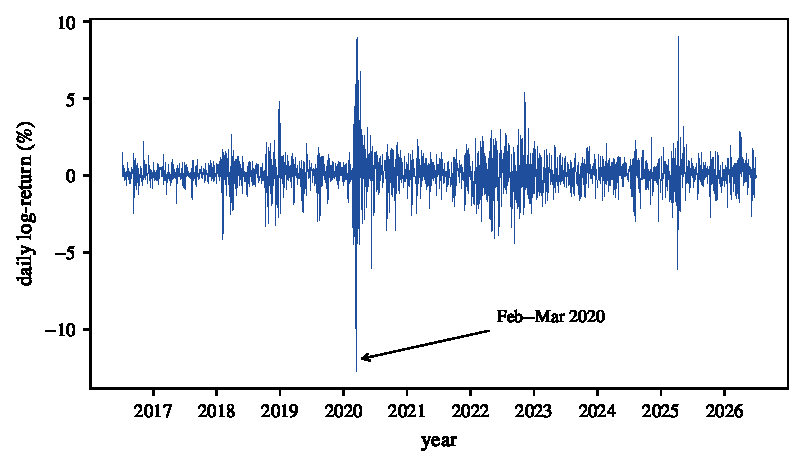
\includegraphics[width=0.9\textwidth]{images/sp500_logreturns.pdf}
\caption{Daily log-returns of the S\&P\,500, 2016--2026 (FRED series SP500). Quiet stretches alternate with bursts of turbulence --- most dramatically the COVID crash of February--March 2020 --- and large returns of either sign cluster together: this is volatility clustering, incompatible with a constant $\sigma$. Generated by \texttt{images/code\_for\_images/sp500\_returns.py}.}
\label{fig:sp500-clustering}
\end{figure}
The log-returns themselves are essentially uncorrelated,
\begin{equation}
\mathbb{E}[dX_i \cdot dX_{i+\tau}] \approx 0 \quad (\text{decaying within minutes}),
\end{equation}
as the EMH demands --- if returns were predictable, they would be arbitraged away.
But their \emph{absolute values} are strongly and persistently correlated, with a slow power-law decay of the autocorrelation,
\begin{equation}
\mathbb{E}\bigl[|dX_i| \cdot |dX_{i+\tau}|\bigr] \sim \tau^{-\beta}, \qquad \beta \approx 0.3,
\end{equation}
% CLAUDE NOTE: the notes (PDF 6, page 5) write "~ τ^β, β ≈ 0.8"; an autocorrelation that
% DECAYS requires a negative exponent, and the measured value for |returns| of the S&P 500
% is β ≈ 0.3 (Gopikrishnan et al. 1999, as in the course slides). Corrected at the
% author's request (2026-07-06).
so a large move today makes large moves likely for days and weeks to come, in either direction\cite{Gopikrishnan1999}.
Figure~\ref{fig:sp500-acf} shows both facts at once on our daily data: the autocorrelation of the returns collapses into the statistical noise band within a lag or two, while that of the absolute returns stays positive for months, decaying along the $\tau^{-0.3}$ line.

% Figure after the course slides; generated by images/code_for_images/sp500_stylized.py
\begin{figure}[h!]
\centering
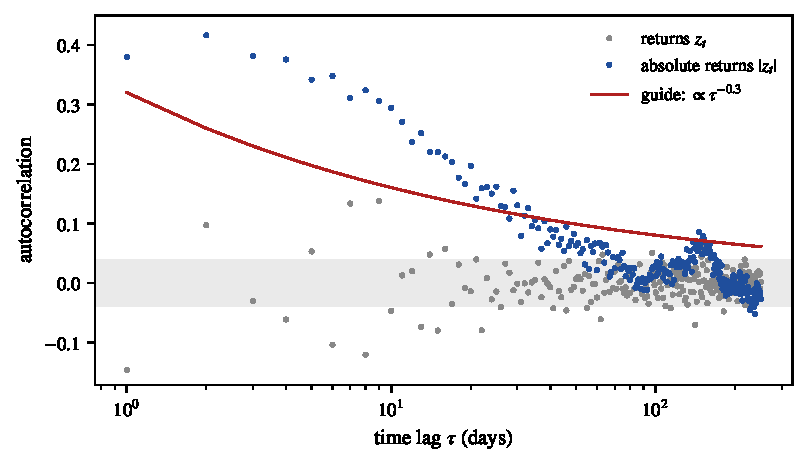
\includegraphics[width=0.85\textwidth]{images/sp500_acf.pdf}
\caption{Sample autocorrelation of the daily S\&P\,500 log-returns (grey) and of their absolute values (blue), against the time lag $\tau$; the shaded band is the $95\%$ noise level. Returns are uncorrelated beyond a day --- efficient-market behaviour --- while their magnitudes remain correlated for months, with the power-law decay $\propto\tau^{-0.3}$ (red): returns are uncorrelated but not independent. Generated by \texttt{images/code\_for\_images/sp500\_stylized.py}.}
\label{fig:sp500-acf}
\end{figure}
The two facts together imply that
\begin{equation}
\sigma_{\text{hf}}^2 \neq \sigma_{\text{ist}}^2,
\end{equation}
i.e.\ the log-returns, though uncorrelated, are \emph{not independent} --- the dependence hides in their magnitudes.
This is \emph{volatility clustering}, and it kills the constant-$\sigma$ hypothesis for good; even the distribution of the volatility itself turns out to have heavy tails, and is well fitted empirically by a log-normal or an inverse-Gamma law\cite{BouchaudPotters2003}.
% CLAUDE NOTE: the log-normal / inverse-Gamma fits are from the course slides
% (after Bouchaud & Potters), added 2026-07-06.
The natural response is to give $\sigma$ its own dynamics.


\section[Fractional Brownian motion*]{Fractional Brownian motion\texorpdfstring{$^*$}{*}}\label{sec:fbm}
% ============================================================================
% SECTION WRITTEN FROM SCRATCH (asterisk convention): "moto browniano frazionario"
% is listed in the official course program ("slides and other/programma.pdf",
% section "Dinamica dei Mercati Finanziari") but does not appear in the handwritten
% notes; only a passing mention of fractional models survives in the slides.
% Written 2026-07-06 from Mandelbrot & Van Ness (1968) and Gatheral et al. (2018).
% ============================================================================

Before turning correlated volatility into a model, it is worth meeting the stochastic process invented precisely to carry \emph{long-range memory}: the \emph{fractional Brownian motion} (fBM) of Mandelbrot and Van~Ness\cite{MandelbrotVanNess1968}.
The Wiener process of Chapter~3 has independent increments by construction; fBM relaxes exactly this axiom, and nothing else.
It is the Gaussian process $B_H(t)$ with $B_H(0)=0$, zero mean, and covariance
\begin{equation}
\langle B_H(t)\, B_H(s)\rangle = \frac{1}{2}\bigl(t^{2H} + s^{2H} - |t-s|^{2H}\bigr),
\end{equation}
where the parameter $H\in(0,1)$ is called the \emph{Hurst exponent}.
For $H=\tfrac12$ the covariance collapses to $\min(t,s)$, and one recognizes the autocorrelation of the ordinary Wiener process: fBM is a one-parameter deformation of Brownian motion, with $H$ dialling the memory.

Three properties follow directly from the covariance.
First, the variance grows \emph{anomalously},
\begin{equation}
\mathrm{Var}[B_H(t)] = t^{2H},
\end{equation}
faster than linearly for $H>\tfrac12$ (superdiffusion) and slower for $H<\tfrac12$ (subdiffusion) --- the process is self-similar with exponent $H$, generalizing the $\sqrt{t}$ scaling of Chapter~2.
Second, the increments are stationary but \emph{correlated}: a short computation with the covariance shows that the correlation of two successive unit increments equals $2^{2H-1}-1$, which is positive for $H>\tfrac12$ (\emph{persistence}: a rise tends to be followed by a rise), negative for $H<\tfrac12$ (\emph{antipersistence}: a rise tends to be followed by a fall), and zero only at $H=\tfrac12$.
Third --- and this is the price of memory --- for $H\neq\tfrac12$ the process is \emph{neither Markov nor a semimartingale}: the entire framework of Chapters~3 and~4, from Chapman--Kolmogorov to the It\^o integral, does not apply to it as it stands.
Long-range dependence is bought at the cost of the whole toolbox.

Why pay that price?
Because the volatility, as we have just measured, \emph{has} long-range memory: the power-law decay of Figure~\ref{fig:sp500-acf} is precisely the kind of correlation that no Markov process can sustain and that fBM carries natively.
The modern \emph{rough volatility} programme models the log-volatility as a fractional Brownian motion, and the empirical estimates are striking: fitting high-frequency data gives a very small Hurst exponent, $H\approx0.1$ --- volatility is not only stochastic but \emph{rough}, far more irregular than a Brownian path --- while reproducing the smile and the clustering with remarkably few parameters\cite{GatheralEtAl2018}.
For the underlying price itself, on the other hand, $H\ne\tfrac12$ would imply predictable returns and hence arbitrage, so the EMH pins the price's Hurst exponent to $\tfrac12$; the memory lives in the volatility, not in the direction of the moves --- in exact agreement with the two panels of Figure~\ref{fig:sp500-acf}.


\section{Stochastic volatility models}\label{sec:stoch-vol}

To model a time-varying $\sigma$, one couples the price to a second stochastic process $Y(t)$ that drives the volatility.
The general \emph{stochastic volatility} model is the two-dimensional SDE system
\begin{align}
(1)\quad & dS(t) = \mu\, S(t)\, dt + f[Y(t)]\, S(t)\, dW_1(t), \label{eq:sv-stock} \\[4pt]
(2)\quad & dY(t) = \alpha\bigl(m - Y(t)\bigr)dt + g[Y(t)]\, dW_2(t), \label{eq:sv-vol}
\end{align}
whose ingredients deserve individual introductions.
The function $f[Y(t)]$ converts the auxiliary process into the actual volatility of the stock, $\sigma(t)=f[Y(t)]$; its choice distinguishes the models below.
The drift of $Y$ is of Ornstein--Uhlenbeck type, so the volatility is \emph{mean-reverting} --- pushed up or down toward its long-run level $m$, in agreement with the observed alternation of calm and turbulent regimes.
The function $g[Y(t)]$ is the noise amplitude of the volatility itself, universally known as the \emph{vol of vol}.
Finally --- and this is the empirically crucial ingredient --- the two Wiener processes are \emph{correlated}, with coefficient $\rho \in [-1,1]$:
\begin{equation}
dW_2(t) = \rho\, dW_1(t) + \sqrt{1-\rho^2}\, dZ(t),
\end{equation}
where $Z$ is a Wiener process independent of $W_1$.
Let us verify that $W_2$ so defined is a legitimate Wiener process.
Its increments have zero mean,
\begin{equation}
\mathbb{E}[dW_2] = \rho\,\mathbb{E}[dW_1] + \sqrt{1-\rho^2}\,\mathbb{E}[dZ] = 0,
\end{equation}
and the correct variance,
\begin{equation}
\mathbb{E}[dW_2^2] = \rho^2\,\mathbb{E}[dW_1^2] + (1-\rho^2)\,\mathbb{E}[dZ^2] = \rho^2\,dt + (1-\rho^2)\,dt = dt,
\end{equation}
while the cross-correlation with $W_1$ is, by construction,
\begin{equation}
\langle dW_1(t)\, dW_2(t)\rangle = \rho\, dt.
\end{equation}
Empirically $\rho<0$ for equities (fits give $\rho\approx-0.7$ for stock indices): when the price falls, the volatility rises --- bad news makes the market panic.
This asymmetry is the \emph{leverage effect}, so named from its first interpretation in terms of firms' debt leverage, and its fingerprints were all over the crises of 2007--2008.

\subsection{Specific models}

Different choices of the pair $(f,g)$ define the models found in the literature, of which three are canonical.

\begin{enumerate}
    \item \textbf{Stein--Stein}\cite{SteinStein1991}: $f[Y] = Y = \sigma$ and $g[Y] = \kappa > 0$, so the volatility itself follows a classical Gaussian OU process,
    \begin{equation}
    d\sigma = \alpha(m-\sigma)\,dt + \kappa\, dW_2,
    \end{equation}
    stationary from $-\infty$ to $+\infty$ with distribution $\mathcal{N}(\sigma)$.
    Simplicity has a price: a Gaussian $\sigma$ can go negative, and one must force positivity by taking $|\sigma|$.

    \item \textbf{Heston}\cite{Heston1993}: $f[Y] = \sqrt{Y}$ and $g[Y] = \kappa\sqrt{Y}$, so that the \emph{variance} $v=\sigma^2$ follows
    \begin{equation}
    d\sigma^2 = \alpha(m-\sigma^2)\,dt + \kappa\sqrt{\sigma^2}\, dW_2(t),
    \end{equation}
    which is exactly a CIR process (Chapter~6) for $\sigma^2$: its distribution is $\mathrm{PDF}\{\sigma^2\}=\chi^2(\sigma^2)$, \emph{positive by construction}.
    This built-in positivity, together with a semi-analytical option-pricing formula, has made Heston the industry standard.

    \item \textbf{Exponential OU} (Scott): $f[Y] = e^Y$, so $\sigma = e^Y > 0$, with $g[Y] = \kappa$ and
    \begin{equation}
    dY = \alpha(m-Y)\,dt + \kappa\, dW_2(t), \qquad \mathrm{PDF}\{\sigma\} = \mathrm{LN}(\sigma),
    \end{equation}
    a log-normal volatility: positive as well, but difficult to treat analytically.
\end{enumerate}

The frontier has since moved on: recent models replace the driving noise with \emph{fractional} Brownian motion, rougher and more irregular than the standard one, in the ``rough volatility'' program.
A sobering general remark closes the survey: for none of these models is the PDF of the returns known in closed form.
What is known is the phenomenology --- leptokurtic, fat-tailed distributions at high frequency, slowly re-Gaussianizing over long horizons (the \emph{aggregational Gaussianity} of the stylized-facts literature\cite{Cont2001}) --- which is precisely what the data show, and what the GBM could not produce.


\section{Option pricing under Heston's model}\label{sec:heston-pricing}
% CLAUDE NOTE: this section was rewritten on 2026-07-06 to follow the handwritten notes
% (PDF 6, page 6) strictly, after the author pointed out that the earlier draft had
% misread them: the strikethroughs in the notes cancel the μS terms (they are not
% errors), the notes' "rapporto vega" label for Δ₁ is correct, and the exposition below
% now mirrors the notes line by line. Per the author's permission, the notation is that
% of Heston's original paper: κ (mean reversion), θ (long-run variance), σ (vol of vol);
% the notes write γ(θ−v)dt + κ√v dW₂ for the same objects. The maturity ordering is
% T₁ > T₂ ≥ t (the notes write T₁ > T₂ > t; "≥" fixed at the author's request).

Does the Black--Scholes program survive stochastic volatility?
The Heston model (1993)\cite{Heston1993} is the natural laboratory, being the direct generalization of Black--Scholes:
\begin{align}
dS &= \mu\, S\, dt + \sqrt{v}\, S\, dW_1, \label{eq:heston-S} \\
dv &= \kappa(\theta - v)\, dt + \sigma\sqrt{v}\, dW_2, \label{eq:heston-v}
\end{align}
where $v$ is the variance and $\langle dW_1\, dW_2\rangle = \rho\, dt$, the correlation being realized through the buying and selling of the stock itself.
Figure~\ref{fig:heston-sim} shows what the model produces: price paths of realistic roughness, driven by a volatility that is itself a fluctuating, mean-reverting process.

% Figure after the course slides (Econophysics of the Financial Market Dynamics);
% generated by images/code_for_images/heston_sim.py
\begin{figure}[h!]
\centering
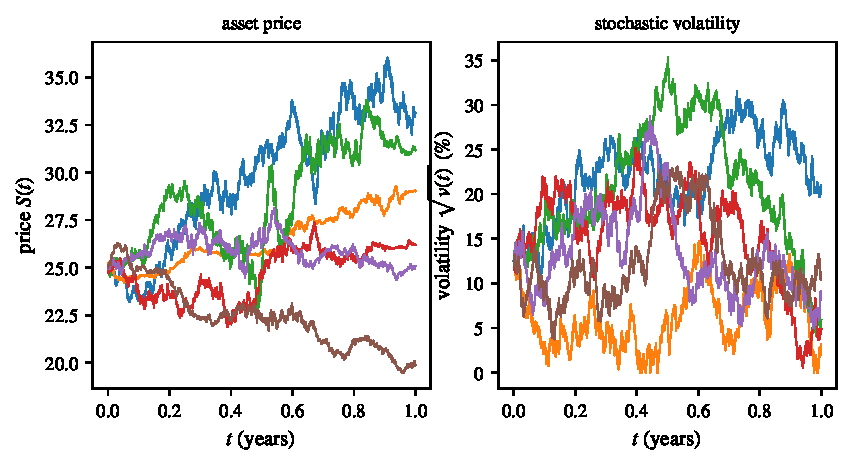
\includegraphics[width=0.95\textwidth]{images/heston_sim.pdf}
\caption{Monte Carlo simulation of the Heston model (six sample paths, full-truncation Euler scheme): the asset price $S(t)$ (left) and its stochastic volatility $\sqrt{v(t)}$ (right), with negative price--volatility correlation $\rho=-0.125$ to account for the leverage effect. Simulations of this kind are routinely used in finance for the pricing of plain vanilla and exotic options under stochastic volatility. Generated by \texttt{images/code\_for\_images/heston\_sim.py}.}
\label{fig:heston-sim}
\end{figure}

In Black--Scholes only the price $S(t)$ moves, and one protects oneself by holding stock.
In Heston one still hedges $dW_1$ by buying $S$, but for $dW_2$ there is nothing to buy: volatility is not exchanged.
One therefore needs another instrument, sensitive to volatility \emph{and} tradable --- another option.

\subsection{Hedging with two options}

Consider then two options $O_1$ and $O_2$ on the same stock, with maturities $T_1$ and $T_2$: $O_2$ is the \emph{target} option, the one the writer has sold, and $O_1$ is the instrument used to cover $dW_2$, with
\begin{equation}
T_1 > T_2 \ge t
\end{equation}
(the hedging option must outlive the target).
% CLAUDE NOTE: the notes write T₁ > T₂ > t; corrected to T₁ > T₂ ≥ t at the author's
% request (2026-07-06).
The writer's wealth is a portfolio of cash, a fraction $\Delta$ of stock (which takes care of $dW_1$), and a fraction $\Delta_1$ of the hedging option (which takes care of $dW_2$),
\begin{equation}
W(S,v,t) = \Pi(S,v,t) + \underbrace{\Delta(S,v,t)\, S}_{dW_1} + \underbrace{\Delta_1(S,v,t)\, O_1(S,v,t)}_{dW_2}
= O_2(S,v,t), \qquad \Delta, \Delta_1 \in \mathbb{R},
\end{equation}
where the last equality is replication: the portfolio must reproduce the sold option.
Therefore
\begin{equation}
\Pi(S,v,t) = O_2 - \Delta\, S - \Delta_1\, O_1
\quad\Longrightarrow\quad
d\Pi = dO_2 - \Delta\, dS - \Delta_1\, dO_1.
\end{equation}

To expand $dO_1$ and $dO_2$ we need the \emph{two-dimensional It\^o formula}, the natural extension of~\eqref{eq:ito-formula}: for $f[X(t), Y(t), t]$ with $dX = a\, dt + b\, dW_1$ and $dY = c\, dt + d\, dW_2$,
\begin{equation}
df = \biggl(\frac{\partial f}{\partial t} + a\frac{\partial f}{\partial x} + c\frac{\partial f}{\partial y} + \frac{1}{2}b^2\frac{\partial^2 f}{\partial x^2} + \frac{1}{2}d^2\frac{\partial^2 f}{\partial y^2} + \rho\, b\, d\,\frac{\partial^2 f}{\partial x\,\partial y}\biggr)dt + b\frac{\partial f}{\partial x}\, dW_1 + d\frac{\partial f}{\partial y}\, dW_2,
\end{equation}
the only novelty being the mixed term, generated by $dW_1\,dW_2 = \rho\,dt$.
Applied to the two option prices, and collecting the second-order operators into
\begin{equation}
\mathcal{D} = \frac{1}{2}v\, S^2\frac{\partial^2}{\partial S^2} + \frac{1}{2}\sigma^2 v\frac{\partial^2}{\partial v^2} + \rho\,\sigma\, v\, S\frac{\partial^2}{\partial S\,\partial v},
\end{equation}
this gives, for $i=1,2$,
\begin{equation}
dO_i = \biggl\{\frac{\partial O_i}{\partial t} + \mu S\frac{\partial O_i}{\partial S} + \kappa(\theta - v)\frac{\partial O_i}{\partial v} + \mathcal{D}\, O_i\biggr\}dt
+ \sqrt{v}\, S\,\frac{\partial O_i}{\partial S}\, dW_1
+ \sigma\sqrt{v}\,\frac{\partial O_i}{\partial v}\, dW_2.
\end{equation}

Now rearrange the portfolio differential as $d\Pi + \Delta\, dS + \Delta_1\, dO_1 = dO_2$ and compare the noise terms on the two sides.
Collecting $dW_1$ on the left gives $\sqrt{v}\,S\bigl(\Delta + \Delta_1\,\partial_S O_1\bigr)\,dW_1$, while the right carries $\sqrt{v}\,S\,\partial_S O_2\, dW_1$; collecting $dW_2$ gives $\Delta_1\,\sigma\sqrt{v}\,\partial_v O_1\, dW_2$ against $\sigma\sqrt{v}\,\partial_v O_2\, dW_2$.
The noise $dW_2$ cancels between the two members if
\begin{equation}
\sigma\sqrt{v}\,\frac{\partial O_2}{\partial v} = \Delta_1\,\sigma\sqrt{v}\,\frac{\partial O_1}{\partial v}
\quad\Longrightarrow\quad
\Delta_1 = \frac{\partial O_2/\partial v}{\partial O_1/\partial v}
\qquad \text{(the \emph{vega ratio})},
\end{equation}
the optimal option fraction: the two options are held in proportion to their volatility sensitivities, and the volatility noise is gone.
Likewise for $dW_1$,
\begin{equation}
\sqrt{v}\, S\,\frac{\partial O_2}{\partial S} = \sqrt{v}\, S\biggl(\Delta + \Delta_1\frac{\partial O_1}{\partial S}\biggr)
\quad\Longrightarrow\quad
\Delta = \frac{\partial O_2}{\partial S} - \Delta_1\frac{\partial O_1}{\partial S},
\end{equation}
the optimal stock fraction: the familiar delta hedge, with a \emph{correction} for the delta carried along by the hedging option.

\subsection{The Heston PDE}

With both noises cancelled, $d\Pi$ is now riskless, and by the no-arbitrage principle it must earn the risk-free rate,
\begin{equation}
d\Pi = r\,\Pi\, dt = r\,\bigl\{O_2 - \Delta\, S - \Delta_1\, O_1\bigr\}\,dt,
\end{equation}
with the optimal $\Delta$ and $\Delta_1$ substituted in.
On the other hand, $d\Pi$ can be computed from the It\^o expansions of $dO_1$ and $dO_2$ above; when the two expressions are equated, every term proportional to $\mu S$ cancels identically between the $O_2$ terms, the stock term, and the $O_1$ terms --- the same disappearance of the historical drift that blessed the Black--Scholes derivation.
% CLAUDE NOTE: these cancellations are exactly what the strikethrough marks in the
% handwritten notes (PDF 6, page 6) indicate.
What survives can be separated so that everything referring to $O_1$ stands on one side and everything referring to $O_2$ on the other:
\begin{equation}\begin{split}
&\biggl\{\frac{\partial O_1}{\partial t} + rS\frac{\partial O_1}{\partial S} + \kappa(\theta - v)\frac{\partial O_1}{\partial v} + \mathcal{D} O_1 - r O_1\biggr\}\biggl(\frac{\partial O_1}{\partial v}\biggr)^{\!-1}\\
&\qquad= \biggl\{\frac{\partial O_2}{\partial t} + rS\frac{\partial O_2}{\partial S} + \kappa(\theta - v)\frac{\partial O_2}{\partial v} + \mathcal{D} O_2 - r O_2\biggr\}\biggl(\frac{\partial O_2}{\partial v}\biggr)^{\!-1},
\end{split}\end{equation}
that is,
\begin{equation}
\frac{\mathrm{drift}(O_1) - r O_1}{\mathrm{vega}(O_1)} = \frac{\mathrm{drift}(O_2) - r O_2}{\mathrm{vega}(O_2)} = \lambda(S,v,t),
\end{equation}
a \emph{universal} function, the same for every option on this stock whatever its maturity --- the same separation-of-variables manoeuvre that produced the Vasi\v{c}ek identity in Chapter~6.
The function $\lambda$ is the \emph{price of volatility risk}: the extra return demanded per unit of volatility exposure, the exact analogue of the market price of risk $q$ of Chapter~6, and it appears here for the same reason as there --- because the risk source ($v$, like $r$) is not tradable.

Undoing the ratio, every option price must satisfy the \textbf{Heston PDE}:
\begin{equation}\label{eq:heston-pde}
\boxed{\ \underbrace{\frac{\partial O}{\partial t} + rS\frac{\partial O}{\partial S} + \frac{1}{2}vS^2\frac{\partial^2 O}{\partial S^2}}_{\text{Black--Scholes}} + \rho\,\sigma\, v\, S\frac{\partial^2 O}{\partial S\,\partial v} + \kappa(\theta - v)\frac{\partial O}{\partial v} + \frac{1}{2}\sigma^2 v\frac{\partial^2 O}{\partial v^2} - \lambda\frac{\partial O}{\partial v} = r\, O\ }
\end{equation}
The first three terms are exactly Black--Scholes; the new ones are the volatility drift and diffusion, the mixed derivative, and the $-\lambda\,\partial_v O$ term carrying the price of volatility risk (which may equivalently be folded into the drift as $[\kappa(\theta-v)-\lambda]\,\partial_v O$; in practice $\lambda$ is calibrated, or set to zero under the risk-neutral measure).
The equation duly collapses onto Black--Scholes when the volatility freezes ($\sigma=0$, $v=\text{const}$).

Is it solvable?
Remarkably, yes --- analytically, up to one integral.
For a European call the solution retains the Black--Scholes skeleton,
\begin{equation}
C(S,v,t) = S\,P_1 - X\,e^{-r(T-t)}\,P_2 \;\neq\; C_{\text{BS}},
\end{equation}
but the exercise probabilities $P_1$ and $P_2$ are no longer cumulative normals: they are computed numerically as the Fourier-type integrals
\begin{equation}
P_j = \frac{1}{2} + \frac{1}{\pi}\int_0^{\infty} \mathrm{Re}\bigl\{\cdots\bigr\}\, d\phi, \qquad j=1,2,
\end{equation}
whose integrands involve the model's characteristic function.\footnote{Heston's original insight was precisely that, although the PDF of the model is unknown, its \emph{characteristic function} is known in closed form; $P_1$ and $P_2$ then follow by inverse Fourier transform, evaluated by quadrature. This ``transform pricing'' technique has become a small industry of its own.}
The model earns its keep on the data as well: Dr\u{a}gulescu and Yakovenko showed that the Heston return distribution fits the Dow Jones index across time lags from one day to a year, reproducing the fat-tailed short-horizon distributions and their slow re-Gaussianization in one stroke\cite{DragulescuYakovenko2002}.
% CLAUDE NOTE: the Dragulescu-Yakovenko fit is from the course slides
% (Econophysics of the Financial Market Dynamics), added 2026-07-06.

The lesson of the chapter in one line: the market's deviations from Black--Scholes are systematic and measurable, and the models that capture them --- stable laws for the tails, stochastic volatility for the clustering --- remain tractable enough to price with.

\section{Summary: the stylized facts}
% CLAUDE NOTE: summary after the course slides and Cont's review (ReviewCont.pdf in
% "slides and other/"), added 2026-07-06.

It is useful to close the chapter by collecting the empirical regularities met along the way --- the \emph{stylized facts} of financial returns, so called because they hold, with remarkable universality, across markets, epochs, and asset classes\cite{Cont2001}.
\begin{enumerate}
    \item The geometric Brownian motion with constant volatility is not a realistic description of asset price dynamics.
    \item In liquid markets the returns are \emph{uncorrelated} random variables (the sign of efficient-market behaviour), but they are \emph{not independent}: higher-order correlations survive through the volatility.
    \item In the high-frequency limit the distribution of returns is leptokurtic and non-Gaussian, with heavy tails $P(r) \propto r^{-4}$ (the inverse quartic law), and it converges only slowly to a Gaussian over long horizons (\emph{aggregational Gaussianity}).
    \item The volatility is itself a stochastic process, with intermittent fluctuations (volatility clustering), long-range power-law autocorrelation, and a fat-tailed distribution (log-normal or inverse Gamma).
    \item Stochastic volatility models --- Stein--Stein, Heston, exponential OU --- provide a realistic description of these facts, give rise dynamically to non-Gaussian return distributions, and remain tractable enough for pricing, volatility forecasting, and simulation.
\end{enumerate}
One last application of the Fokker--Planck machinery awaits, and it takes us out of the market altogether: the distribution of wealth in a society.


\chapter{Econophysics, Equilibrium, and Pareto}

This final chapter applies the Fokker--Planck formalism to a problem outside the financial markets: the \emph{distribution of wealth} in a population.
It is, in a sense, the purest piece of econophysics in the book --- no contracts, no hedging, just a statistical-mechanics question asked of society: if incomes diffuse randomly under simple rules, what stationary distribution do they reach?
The answer turns out to reproduce, from one and the same equation, the two regimes observed in every real economy: an exponential (Boltzmann) distribution for the lower and middle class, and a power-law (Pareto) tail for the rich.
% CLAUDE NOTE (unreviewed): These are the last two pages of PDF 6, unreviewed but
% clear in intent. Expansions and footnotes have been added for completeness.


\section{Power laws in economics}

Many phenomena, in economics and beyond, follow a \emph{power law}.
The classic example is \emph{Zipf's law}: rank the words of a text by frequency, and the frequency falls off as a power of the rank.
The same pattern appears in the sizes of cities, the sizes of firms, and --- the case that concerns us --- the distribution of wealth.

Wealth itself is hard to observe, so in practice one uses the \emph{gross income} $r$ (reddito) as a proxy, and studies the complementary CDF --- the fraction of individuals with income at least $r$ --- rescaled by the mean income $r/\bar r$ to compare across countries and years.
When this is done, the data speak clearly: two groups emerge.
The bulk of the population --- the lower and middle class --- follows an \emph{exponential} law; the wealthiest few percent follow a \emph{power-law} (Pareto) tail.
Figure~\ref{fig:wealth-dist} shows the two regimes in the form in which they appear in the empirical literature: in a log-linear plot the exponential bulk is a straight line from which the tail lifts off; in a log-log plot the Pareto tail is a straight line into which the bulk bends.
The power-law tail was discovered by Pareto in 1897\cite{Pareto1897}; the two-regime structure has been confirmed on modern data by Fujiwara, Champernowne, Yakovenko, and many others\cite{Yakovenko2009}, and its remarkable stability across countries and decades cries out for a mechanism.

% Figure replacing the multi-panel plot pasted in the raw notes (page 7);
% generated by images/code_for_images/wealth_distribution.py with parameters
% from Yakovenko & Rosser, Rev. Mod. Phys. 81, 1703 (2009).
\begin{figure}[h!]
\centering
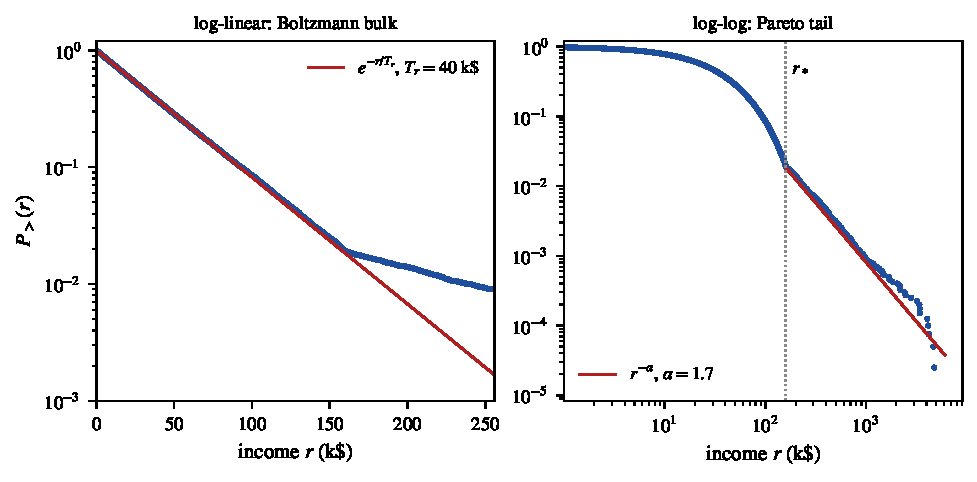
\includegraphics[width=0.95\textwidth]{images/wealth_distribution.pdf}
\caption{The two-regime income distribution, reproduced with the parameters reported for US data by Yakovenko \& Rosser\cite{Yakovenko2009}: an exponential (Boltzmann) bulk with income temperature $T_r\approx\$40$k covering $\sim97\%$ of the population, and a Pareto tail with exponent $\alpha=1.7$ above the crossover $r_*\approx4T_r$. Left, log-linear scale: the bulk is a straight line. Right, log-log scale: the tail is a straight line. Generated by \texttt{images/code\_for\_images/wealth\_distribution.py}.}
\label{fig:wealth-dist}
\end{figure}


\section{A diffusion model for income}\label{sec:income-diffusion}

The mechanism we propose is diffusion: incomes perform a stochastic process in ``income space''.
The physical distinction that will generate the two regimes is the \emph{source} of the income.
For the lower and middle class, income comes from labour --- wages, roughly deterministic, with additive fluctuations.
For the upper class, income comes from \emph{assets} --- capital gains, intrinsically stochastic, with fluctuations proportional to the capital itself.
One model, two regimes of its coefficients.

\subsection{General hypotheses}

The framework rests on four hypotheses.
\begin{enumerate}
    \item Incomes are divisible into an infinitely numerable set of income classes $r \in R_+$, with $r \ge r_{\min}$.
    \item $P(r,t)$ is the fraction of individuals with income $r$ at time $t$, and $N$ is the total number of income earners, so that $N\, P(r,t)\, dr = dm(r,t)\, dr$ counts the earners in $[r,r+dr]$.
    We take $N$ constant, since there is approximately a one-to-one map between individuals and income positions (people change salary, change job, inherit --- but the slots remain).
    \item The distribution is normalized, $\int P(r',t)\, dr' = 1$.
    \item The diffusion has \emph{no memory}: the process is Markov.
\end{enumerate}

\subsection{The master equation}

By hypothesis 4 and the results of Chapter~3, the master equation for $P(r,t)$ is a Fokker--Planck equation, with drift and diffusion coefficients $A(r)$ and $B(r)$:
\begin{equation}\label{eq:fp-income}
\frac{\partial}{\partial t}\, P(r,t) = \frac{\partial}{\partial r}\bigl[A(r)\, P(r,t)\bigr] + \frac{\partial^2}{\partial r^2}\bigl[B(r)\, P(r,t)\bigr],
\end{equation}
written here with the sign convention of the notes, in which
\begin{equation}
\frac{d}{dt}\langle r(t)\rangle = -\langle A(r)\rangle, \qquad \frac{d}{dt}\langle r^2(t)\rangle = \langle 2\,B(r)\rangle:
\end{equation}
a positive $A$ describes an average \emph{loss} of income, and $B$ the intensity of its fluctuations.

\subsection{Equilibrium (stationary) solution}

Now the economic input: empirically, the \emph{shape} of the income distribution is approximately constant over time --- individuals move up and down, but the histogram barely changes from year to year.
This is an equilibrium statement, and we implement it by the \emph{stationary} Fokker--Planck equation,
\begin{equation}
\frac{\partial}{\partial t}\, P(r,t) = 0.
\end{equation}
The right-hand side of~\eqref{eq:fp-income} then collapses into a total derivative,
\begin{equation}
0 = \frac{d}{dr}\bigl[A(r)\, P(r)\bigr] + \frac{d^2}{dr^2}\bigl[B(r)\, P(r)\bigr] = \frac{d}{dr}\biggl\{A(r)\, P(r) + \frac{d}{dr}\bigl[B(r)\, P(r)\bigr]\biggr\},
\end{equation}
and the object in braces is precisely the probability flux $J(r)$ of Chapter~3,
\begin{equation}
J(r) = A(r)\, P(r) + \frac{d}{dr}\bigl[B(r)\, P(r)\bigr],
\end{equation}
constant in $r$ by the equation above.
Requiring $P(r)\to 0$ both as $r\to 0$ and as $r\to\infty$ forces the constant to vanish, so $J=0$ everywhere:
\begin{equation}\label{eq:flux-zero}
A(r)\, P(r) + \frac{d}{dr}\bigl[B(r)\, P(r)\bigr] = 0.
\end{equation}
Equilibrium with zero flux --- detailed balance, a statistical mechanician would say (Appendix~\ref{app:stationary}) --- is a first-order ODE for $P(r)$: given any choice of $A$ and $B$, the stationary distribution follows by one integration.
It remains to feed in the economics.


\section{Lower and middle class}\label{sec:lower-class}

For the lower and middle class both coefficients are constants,
\begin{equation}
A(r) = A_0, \qquad B(r) = B_0 > 0.
\end{equation}
The reading is concrete.
A constant, positive $A_0$ describes a steady linear erosion of purchasing power, $\frac{d}{dt}\langle r(t)\rangle = -A_0$ --- wages nibbled by inflation, taxes, and living costs --- while the fluctuations have constant intensity, $\frac{d}{dt}\langle r^2(t)\rangle = 2B_0$: raises, job changes, small windfalls, all of a size that does not depend on how rich one already is.
This additivity is the statistical signature of \emph{labour} income.

With constant coefficients the stationary equation~\eqref{eq:flux-zero} becomes
\begin{equation}
A_0\, P(r) + B_0\,\frac{dP}{dr} = 0 \quad\Longrightarrow\quad \frac{dP}{P} = -\frac{A_0}{B_0}\, dr,
\end{equation}
and integrating,
\begin{equation}
\int\!\frac{dP(r')}{P(r')} = -\frac{A_0}{B_0}\,r' \quad\Longrightarrow\quad P(r) \propto C\, e^{-\frac{A_0}{B_0}\, r} = C\, e^{-r/T_r},
\end{equation}
an \emph{exponential} distribution (positive and normalizable provided $A_0 > 0$), with scale
\begin{equation}\label{eq:boltzmann-income}
T_r = \frac{B_0}{A_0}.
\end{equation}
The form is unmistakable to a physicist: it is a Boltzmann distribution (Appendix~\ref{app:ensembles}), $e^{-E/k_BT}$ with income in place of energy, and $T_r$ plays the role of an \emph{effective temperature of income} --- large when fluctuations ($B_0$) are strong relative to erosion ($A_0$); the general mechanism by which a zero-flux state of a diffusion acquires the Boltzmann form is spelled out in Appendix~\ref{app:stationary}.
At equilibrium the distribution is stable even though every individual income keeps fluctuating; and if the mean income $\langle r\rangle$ falls, the ``temperature'' falls with it, compressing the whole distribution.
Money, in this class, behaves like energy in a gas: exchanged in roughly equal quanta, conserved overall, and exponentially distributed at equilibrium.


\section{Upper class}\label{sec:upper-class}

For the upper class the phenomenology is different in kind, not just in degree: income is driven by \emph{multiplicative feedback}, because capital generates returns proportional to itself.
The coefficients that encode this are
\begin{equation}
A(r) = a\,r, \qquad B(r) = b\,r^2 \qquad (a, b > 0),
\end{equation}
giving
\begin{equation}
\frac{d}{dt}\langle r(t)\rangle = -a\,\langle r(t)\rangle,
\qquad
\frac{d}{dt}\langle r^2(t)\rangle = b\,\langle r^2(t)\rangle:
\end{equation}
the average relative erosion is the same as before, but the fluctuations now \emph{grow with the square of the income} --- positive feedback, the rich man's gains and losses both scaling with his fortune.
This multiplicativity is the statistical signature of \emph{asset} income, and the reader will recognize in $A\propto r$, $B\propto r^2$ the drift-diffusion structure of the geometric Brownian motion of Chapter~4.

We solve the stationary equation~\eqref{eq:flux-zero} with these coefficients.
Expanding the derivative,
\begin{equation}
A(r)\, P(r) + B(r)\,\frac{dP}{dr} + P(r)\,\frac{dB}{dr} = 0
\quad\Longrightarrow\quad
P'(r) + \frac{A(r) + B'(r)}{B(r)}\, P(r) = 0,
\end{equation}
and substituting $A(r) = ar$, $B(r) = br^2$, $B'(r) = 2br$,
\begin{equation}
P'(r) + \frac{ar + 2br}{br^2}\, P(r) = 0 \quad\Longrightarrow\quad P'(r) + \frac{a+2b}{b}\,\frac{1}{r}\, P(r) = 0.
\end{equation}
This is again a separable first-order ODE,
\begin{equation}
\frac{dP}{P} = -\frac{a+2b}{b}\,\frac{dr}{r},
\end{equation}
whose integral is worth organizing as in the notes: splitting the coefficient as $\frac{a+2b}{b} = \frac{a}{b} + 2$,
\begin{equation}
\int\!\frac{dP(r')}{P(r')} = -\int\!\frac{B'(r')}{B(r')}\, dr' - \int\!\frac{A(r')}{B(r')}\, dr',
\end{equation}
the first integral gives $\ln B(r) = \ln(br^2)$, and the second
\begin{equation}
\int\!\frac{A(r')}{B(r')}\, dr' = \frac{a}{b}\int\!\frac{dr'}{r'} = \frac{a}{b}\,\ln r,
\end{equation}
so that, for $r \gg r_0$,
\begin{equation}
P(r) \approx \frac{C}{B(r)}\, e^{-\int \frac{A(r')}{B(r')}\, dr'} = \frac{C}{b\,r^2}\, r^{-a/b},
\end{equation}
that is,
\begin{equation}\label{eq:pareto}
P(r) = C\, r^{-(2 + a/b)} = C\, r^{-(\alpha+1)},
\end{equation}
a \emph{power law}: the multiplicative structure has converted the exponential into a Pareto tail.
% CLAUDE NOTE: the notes write P(r) = C r^{-2} r^{-a/b} = C r^{-(1+a/b)-1} = C r^{-(1+α)},
% consistent with a CDF exponent α = 1 + a/b as stated below.
Correspondingly, the complementary CDF decays as $r^{-\alpha}$, with
\begin{equation}\label{eq:pareto-exponent}
\alpha = 1 + \frac{a}{b},
\end{equation}
the \textbf{Pareto exponent}.
Since $a, b > 0$, the model predicts $\alpha > 1$ automatically.
Empirically, fits across countries give $\alpha \approx 1.6$--$1.8$, which through~\eqref{eq:pareto-exponent} implies $b > a$: for the upper class, the multiplicative fluctuations of capital \emph{dominate} its average erosion --- and it is precisely this dominance of noise that populates the far tail of great fortunes.\footnote{A Pareto exponent $\alpha < 2$ means that the \emph{variance} of the income distribution diverges: inequality in the tail is so extreme that no ``typical spread'' exists. That $\alpha$ falls in the same narrow window for very different countries suggests that the mechanism --- multiplicative dynamics of capital --- is universal, largely indifferent to institutional detail.}

\medskip

It is worth stepping back to admire the unity of the result.
One Fokker--Planck equation, one zero-flux equilibrium condition; additive coefficients give Boltzmann's exponential for the many, multiplicative coefficients give Pareto's power law for the few, and the crossover between the two regimes is visible in the income data of every country.
The tools were exactly those of the rest of the book --- the same stationary Fokker--Planck equation that priced no options and hedged no portfolios here draws, with two lines of algebra, the statistical portrait of a society.
This is econophysics at its best: not finance dressed up in physics notation, but the genuine transfer of a physical way of thinking --- equilibrium, diffusion, universality --- to economic matter.


\section[The minority game*]{The minority game\texorpdfstring{$^*$}{*}}
% ============================================================================
% BLANK SECTION (placeholder, added at the author's request on 2026-07-06).
% Planned content: the Minority Game of Challet & Zhang (1997) as the agent-based
% counterpart of this chapter — N adaptive agents, public information α = P/N,
% the volatility curve σ²/N, the phase transition at α_c ≈ 0.337, and its exact
% solution by the replica method (Challet, Marsili & Zecchina 2000).
% The asterisk marks material beyond the handwritten notes and the course program.
% ============================================================================

\begin{center}
\fbox{\parbox{0.85\textwidth}{%
\textbf{Note:} This section is a placeholder, to be written.
It will present the \emph{minority game} --- the simplest agent-based model of a market of adaptive, heterogeneous, competing agents --- and its phase transition between an efficient and an inefficient phase, solved exactly with the statistical mechanics of disordered systems.
}}
\end{center}



\backmatter
\printbibliography

\end{document}
